% Generated by Sphinx.
\def\sphinxdocclass{report}
\documentclass[a4paper,10pt,english]{sphinxmanual}
\usepackage[utf8]{inputenc}
\DeclareUnicodeCharacter{00A0}{\nobreakspace}
\usepackage[T1]{fontenc}
\usepackage{babel}
\usepackage{times}
\usepackage[Bjarne]{fncychap}
\usepackage{longtable}
\usepackage{sphinx}
\usepackage{multirow}


\title{kafe Documentation}
\date{October 14, 2014}
\release{0.5.2}
\author{D. Savoiu, G. Quast}
\newcommand{\sphinxlogo}{}
\renewcommand{\releasename}{Release}
\makeindex

\makeatletter
\def\PYG@reset{\let\PYG@it=\relax \let\PYG@bf=\relax%
    \let\PYG@ul=\relax \let\PYG@tc=\relax%
    \let\PYG@bc=\relax \let\PYG@ff=\relax}
\def\PYG@tok#1{\csname PYG@tok@#1\endcsname}
\def\PYG@toks#1+{\ifx\relax#1\empty\else%
    \PYG@tok{#1}\expandafter\PYG@toks\fi}
\def\PYG@do#1{\PYG@bc{\PYG@tc{\PYG@ul{%
    \PYG@it{\PYG@bf{\PYG@ff{#1}}}}}}}
\def\PYG#1#2{\PYG@reset\PYG@toks#1+\relax+\PYG@do{#2}}

\expandafter\def\csname PYG@tok@gd\endcsname{\def\PYG@tc##1{\textcolor[rgb]{0.63,0.00,0.00}{##1}}}
\expandafter\def\csname PYG@tok@gu\endcsname{\let\PYG@bf=\textbf\def\PYG@tc##1{\textcolor[rgb]{0.50,0.00,0.50}{##1}}}
\expandafter\def\csname PYG@tok@gt\endcsname{\def\PYG@tc##1{\textcolor[rgb]{0.00,0.27,0.87}{##1}}}
\expandafter\def\csname PYG@tok@gs\endcsname{\let\PYG@bf=\textbf}
\expandafter\def\csname PYG@tok@gr\endcsname{\def\PYG@tc##1{\textcolor[rgb]{1.00,0.00,0.00}{##1}}}
\expandafter\def\csname PYG@tok@cm\endcsname{\let\PYG@it=\textit\def\PYG@tc##1{\textcolor[rgb]{0.25,0.50,0.56}{##1}}}
\expandafter\def\csname PYG@tok@vg\endcsname{\def\PYG@tc##1{\textcolor[rgb]{0.73,0.38,0.84}{##1}}}
\expandafter\def\csname PYG@tok@m\endcsname{\def\PYG@tc##1{\textcolor[rgb]{0.13,0.50,0.31}{##1}}}
\expandafter\def\csname PYG@tok@mh\endcsname{\def\PYG@tc##1{\textcolor[rgb]{0.13,0.50,0.31}{##1}}}
\expandafter\def\csname PYG@tok@cs\endcsname{\def\PYG@tc##1{\textcolor[rgb]{0.25,0.50,0.56}{##1}}\def\PYG@bc##1{\setlength{\fboxsep}{0pt}\colorbox[rgb]{1.00,0.94,0.94}{\strut ##1}}}
\expandafter\def\csname PYG@tok@ge\endcsname{\let\PYG@it=\textit}
\expandafter\def\csname PYG@tok@vc\endcsname{\def\PYG@tc##1{\textcolor[rgb]{0.73,0.38,0.84}{##1}}}
\expandafter\def\csname PYG@tok@il\endcsname{\def\PYG@tc##1{\textcolor[rgb]{0.13,0.50,0.31}{##1}}}
\expandafter\def\csname PYG@tok@go\endcsname{\def\PYG@tc##1{\textcolor[rgb]{0.20,0.20,0.20}{##1}}}
\expandafter\def\csname PYG@tok@cp\endcsname{\def\PYG@tc##1{\textcolor[rgb]{0.00,0.44,0.13}{##1}}}
\expandafter\def\csname PYG@tok@gi\endcsname{\def\PYG@tc##1{\textcolor[rgb]{0.00,0.63,0.00}{##1}}}
\expandafter\def\csname PYG@tok@gh\endcsname{\let\PYG@bf=\textbf\def\PYG@tc##1{\textcolor[rgb]{0.00,0.00,0.50}{##1}}}
\expandafter\def\csname PYG@tok@ni\endcsname{\let\PYG@bf=\textbf\def\PYG@tc##1{\textcolor[rgb]{0.84,0.33,0.22}{##1}}}
\expandafter\def\csname PYG@tok@nl\endcsname{\let\PYG@bf=\textbf\def\PYG@tc##1{\textcolor[rgb]{0.00,0.13,0.44}{##1}}}
\expandafter\def\csname PYG@tok@nn\endcsname{\let\PYG@bf=\textbf\def\PYG@tc##1{\textcolor[rgb]{0.05,0.52,0.71}{##1}}}
\expandafter\def\csname PYG@tok@no\endcsname{\def\PYG@tc##1{\textcolor[rgb]{0.38,0.68,0.84}{##1}}}
\expandafter\def\csname PYG@tok@na\endcsname{\def\PYG@tc##1{\textcolor[rgb]{0.25,0.44,0.63}{##1}}}
\expandafter\def\csname PYG@tok@nb\endcsname{\def\PYG@tc##1{\textcolor[rgb]{0.00,0.44,0.13}{##1}}}
\expandafter\def\csname PYG@tok@nc\endcsname{\let\PYG@bf=\textbf\def\PYG@tc##1{\textcolor[rgb]{0.05,0.52,0.71}{##1}}}
\expandafter\def\csname PYG@tok@nd\endcsname{\let\PYG@bf=\textbf\def\PYG@tc##1{\textcolor[rgb]{0.33,0.33,0.33}{##1}}}
\expandafter\def\csname PYG@tok@ne\endcsname{\def\PYG@tc##1{\textcolor[rgb]{0.00,0.44,0.13}{##1}}}
\expandafter\def\csname PYG@tok@nf\endcsname{\def\PYG@tc##1{\textcolor[rgb]{0.02,0.16,0.49}{##1}}}
\expandafter\def\csname PYG@tok@si\endcsname{\let\PYG@it=\textit\def\PYG@tc##1{\textcolor[rgb]{0.44,0.63,0.82}{##1}}}
\expandafter\def\csname PYG@tok@s2\endcsname{\def\PYG@tc##1{\textcolor[rgb]{0.25,0.44,0.63}{##1}}}
\expandafter\def\csname PYG@tok@vi\endcsname{\def\PYG@tc##1{\textcolor[rgb]{0.73,0.38,0.84}{##1}}}
\expandafter\def\csname PYG@tok@nt\endcsname{\let\PYG@bf=\textbf\def\PYG@tc##1{\textcolor[rgb]{0.02,0.16,0.45}{##1}}}
\expandafter\def\csname PYG@tok@nv\endcsname{\def\PYG@tc##1{\textcolor[rgb]{0.73,0.38,0.84}{##1}}}
\expandafter\def\csname PYG@tok@s1\endcsname{\def\PYG@tc##1{\textcolor[rgb]{0.25,0.44,0.63}{##1}}}
\expandafter\def\csname PYG@tok@gp\endcsname{\let\PYG@bf=\textbf\def\PYG@tc##1{\textcolor[rgb]{0.78,0.36,0.04}{##1}}}
\expandafter\def\csname PYG@tok@sh\endcsname{\def\PYG@tc##1{\textcolor[rgb]{0.25,0.44,0.63}{##1}}}
\expandafter\def\csname PYG@tok@ow\endcsname{\let\PYG@bf=\textbf\def\PYG@tc##1{\textcolor[rgb]{0.00,0.44,0.13}{##1}}}
\expandafter\def\csname PYG@tok@sx\endcsname{\def\PYG@tc##1{\textcolor[rgb]{0.78,0.36,0.04}{##1}}}
\expandafter\def\csname PYG@tok@bp\endcsname{\def\PYG@tc##1{\textcolor[rgb]{0.00,0.44,0.13}{##1}}}
\expandafter\def\csname PYG@tok@c1\endcsname{\let\PYG@it=\textit\def\PYG@tc##1{\textcolor[rgb]{0.25,0.50,0.56}{##1}}}
\expandafter\def\csname PYG@tok@kc\endcsname{\let\PYG@bf=\textbf\def\PYG@tc##1{\textcolor[rgb]{0.00,0.44,0.13}{##1}}}
\expandafter\def\csname PYG@tok@c\endcsname{\let\PYG@it=\textit\def\PYG@tc##1{\textcolor[rgb]{0.25,0.50,0.56}{##1}}}
\expandafter\def\csname PYG@tok@mf\endcsname{\def\PYG@tc##1{\textcolor[rgb]{0.13,0.50,0.31}{##1}}}
\expandafter\def\csname PYG@tok@err\endcsname{\def\PYG@bc##1{\setlength{\fboxsep}{0pt}\fcolorbox[rgb]{1.00,0.00,0.00}{1,1,1}{\strut ##1}}}
\expandafter\def\csname PYG@tok@kd\endcsname{\let\PYG@bf=\textbf\def\PYG@tc##1{\textcolor[rgb]{0.00,0.44,0.13}{##1}}}
\expandafter\def\csname PYG@tok@ss\endcsname{\def\PYG@tc##1{\textcolor[rgb]{0.32,0.47,0.09}{##1}}}
\expandafter\def\csname PYG@tok@sr\endcsname{\def\PYG@tc##1{\textcolor[rgb]{0.14,0.33,0.53}{##1}}}
\expandafter\def\csname PYG@tok@mo\endcsname{\def\PYG@tc##1{\textcolor[rgb]{0.13,0.50,0.31}{##1}}}
\expandafter\def\csname PYG@tok@mi\endcsname{\def\PYG@tc##1{\textcolor[rgb]{0.13,0.50,0.31}{##1}}}
\expandafter\def\csname PYG@tok@kn\endcsname{\let\PYG@bf=\textbf\def\PYG@tc##1{\textcolor[rgb]{0.00,0.44,0.13}{##1}}}
\expandafter\def\csname PYG@tok@o\endcsname{\def\PYG@tc##1{\textcolor[rgb]{0.40,0.40,0.40}{##1}}}
\expandafter\def\csname PYG@tok@kr\endcsname{\let\PYG@bf=\textbf\def\PYG@tc##1{\textcolor[rgb]{0.00,0.44,0.13}{##1}}}
\expandafter\def\csname PYG@tok@s\endcsname{\def\PYG@tc##1{\textcolor[rgb]{0.25,0.44,0.63}{##1}}}
\expandafter\def\csname PYG@tok@kp\endcsname{\def\PYG@tc##1{\textcolor[rgb]{0.00,0.44,0.13}{##1}}}
\expandafter\def\csname PYG@tok@w\endcsname{\def\PYG@tc##1{\textcolor[rgb]{0.73,0.73,0.73}{##1}}}
\expandafter\def\csname PYG@tok@kt\endcsname{\def\PYG@tc##1{\textcolor[rgb]{0.56,0.13,0.00}{##1}}}
\expandafter\def\csname PYG@tok@sc\endcsname{\def\PYG@tc##1{\textcolor[rgb]{0.25,0.44,0.63}{##1}}}
\expandafter\def\csname PYG@tok@sb\endcsname{\def\PYG@tc##1{\textcolor[rgb]{0.25,0.44,0.63}{##1}}}
\expandafter\def\csname PYG@tok@k\endcsname{\let\PYG@bf=\textbf\def\PYG@tc##1{\textcolor[rgb]{0.00,0.44,0.13}{##1}}}
\expandafter\def\csname PYG@tok@se\endcsname{\let\PYG@bf=\textbf\def\PYG@tc##1{\textcolor[rgb]{0.25,0.44,0.63}{##1}}}
\expandafter\def\csname PYG@tok@sd\endcsname{\let\PYG@it=\textit\def\PYG@tc##1{\textcolor[rgb]{0.25,0.44,0.63}{##1}}}

\def\PYGZbs{\char`\\}
\def\PYGZus{\char`\_}
\def\PYGZob{\char`\{}
\def\PYGZcb{\char`\}}
\def\PYGZca{\char`\^}
\def\PYGZam{\char`\&}
\def\PYGZlt{\char`\<}
\def\PYGZgt{\char`\>}
\def\PYGZsh{\char`\#}
\def\PYGZpc{\char`\%}
\def\PYGZdl{\char`\$}
\def\PYGZhy{\char`\-}
\def\PYGZsq{\char`\'}
\def\PYGZdq{\char`\"}
\def\PYGZti{\char`\~}
% for compatibility with earlier versions
\def\PYGZat{@}
\def\PYGZlb{[}
\def\PYGZrb{]}
\makeatother

\begin{document}

\maketitle
\tableofcontents
\phantomsection\label{index::doc}

\begin{quote}

\textbf{kafe} is a data fitting framework designed for use in undergraduate
physics lab courses. It provides a basic Python toolkit for fitting
models to data as well as visualisation of the data and the model function.
It relies on Python packages such as \emph{NumPy} and \emph{matplotlib}, and uses
the python interface to the minimizer \emph{Minuit} contained in the data
analysis framework \emph{ROOT}.
\end{quote}


\chapter{\texttt{kafe} Overview}
\label{index:welcome-to-kafe-karlsruhe-fit-environment}\label{index:kafe-overview}\begin{figure}[htbp]\begin{flushright}
\capstart

\scalebox{1.000000}{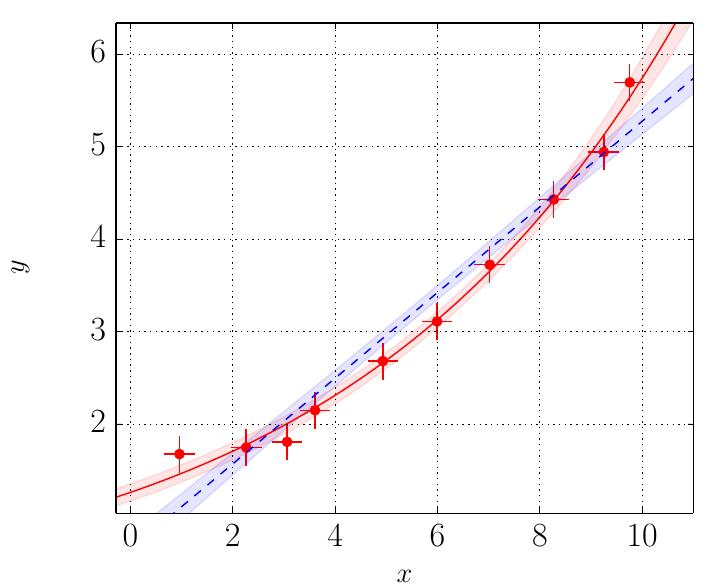
\includegraphics{graph_example1.jpg}}
\caption{\emph{Graphical output generated with kafe}.}\end{flushright}\end{figure}

The \code{kafe} package provides a rather general approach to fitting of a model
function to two-dimensional data points with correlated uncertainties in both
dimensions. A typical use-case would be measurements of two quantities,
an \emph{x}- and a \emph{y}-value, with both uncorrelated (statistical) uncertainties
and correlated systematic uncertainties.

Use cases range from performing a simple average of measurements
to complex situations with correlated uncertainties on the measurements
of the x and y values. The python-API guarantees full flexibility
for data input. Helper functions, which also serve as examples for
own implementations,  are available to handle file-based examples.

The model function describes the y values as a function of the
x-values and a set of model parameters \{p\}, \emph{y=f(x; \{p\})}. Full
flexibility exists as model functions are implemented as
\emph{python} code. Again, examples are provided, but user
implementations are supported as well.

Fitting is based on the \(\chi\)²-method, assuming Gaussian errors and
correlations described by covariance matrices. The level of agreement
between data points and the fit model is expressed in terms of the
\emph{\(\chi\)² probability}, i. e. the probability to find less agreement between
data and model than actually observed. Full access to the covariance
matrix of the - typically correlated - model parameters is provided.

The graphical output visualises the data and the fit model at the
best-fit-point of the parameters and also shows the uncertainty
of the fit model as a light band surrounding the line representing
the model function.


\section{Code Structure}
\label{index:code-structure}\begin{figure}[htbp]\begin{flushright}
\capstart

\scalebox{0.800000}{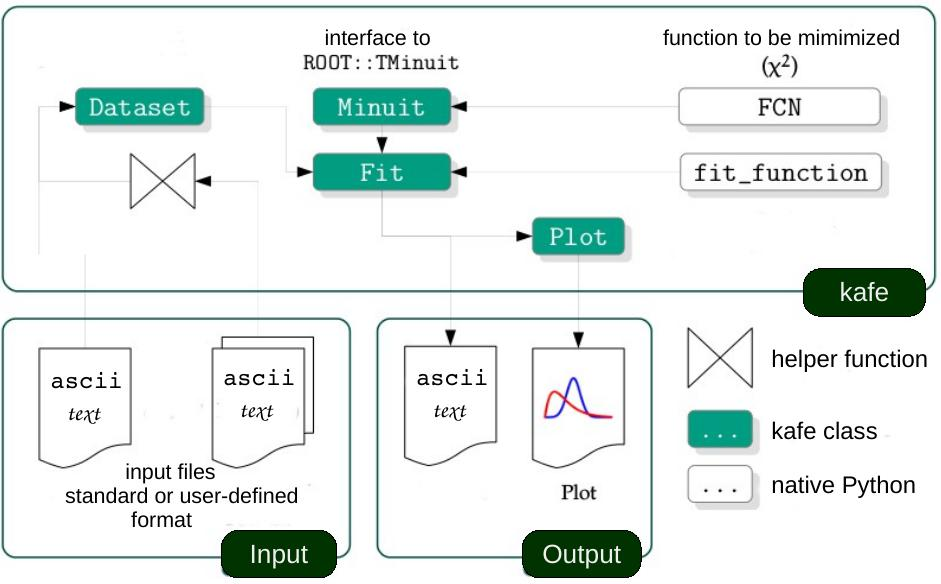
\includegraphics{kafeDiagram.jpg}}
\caption{\emph{Code structure of the kafe package}}\end{flushright}\end{figure}

The code of cafe is centred around very few classes to handle Data input,
fitting and plotting, as illustrated in the figure on the right-hand side.

Data, their uncertainties, and, optionally, the correlations of the
uncertainties - are passed through the interface of the cafe class
\code{Dataset}. Input can be included in the Python code or is read
from files in standardised or user-defined formats. The representation
of the data within the \code{Dataset} class is minimalistic, consisting
of the x and y values and the full covariance matrices of their
uncertainties. Correlated errors between x and y values are not
supported yet, as such use cases are extremely rare.

A helper function, \code{build\_dataset()}, is available
to transform various error models, like a combination of independent
and correlated errors or common absolute or relative errors, to this
basic format.

Adding a model function, taken either from a prepared set of fit
functions within kafe or from a user's own \emph{python} implementation,
results in a \code{Fit} object, which controls the minimizer \code{Minuit}
and provides the results through access methods.

One or multiple fit objects, i. e. the input data and model
functions(s) at the best-fit point in parameter-space, are
visualised by the class \code{Plot} with the help of \emph{matplotlib}
functionality. The \code{plot} module also contains functionality to
display the model uncertainty by surrounding the model function
at the best-fit values of the parameters by a light band, the one-\(\sigma\)
uncertainty band, which is obtained by propagation of the uncertainties
of the fit parameters, taking into account their correlations.


\section{Example}
\label{index:example}
Only very few lines of Python code are needed to perform fits with kafe.
The sniplet of code shown below performs a fit of a quadratic
function to some data points with uncertainties:

\begin{Verbatim}[commandchars=\\\{\}]
\PYG{k+kn}{from} \PYG{n+nn}{kafe} \PYG{k+kn}{import} \PYG{o}{*}
\PYG{k+kn}{from} \PYG{n+nn}{kafe.function\PYGZus{}library} \PYG{k+kn}{import} \PYG{n}{quadratic\PYGZus{}3par}

\PYG{c}{\PYGZsh{}\PYGZsh{}\PYGZsh{}\PYGZsh{} build a Dataset instance:}
\PYG{n}{myDataset} \PYG{o}{=} \PYG{n}{build\PYGZus{}dataset}\PYG{p}{(}
    \PYG{p}{[}\PYG{l+m+mf}{0.05}\PYG{p}{,}\PYG{l+m+mf}{0.36}\PYG{p}{,}\PYG{l+m+mf}{0.68}\PYG{p}{,}\PYG{l+m+mf}{0.80}\PYG{p}{,}\PYG{l+m+mf}{1.09}\PYG{p}{,}\PYG{l+m+mf}{1.46}\PYG{p}{,}\PYG{l+m+mf}{1.71}\PYG{p}{,}\PYG{l+m+mf}{1.83}\PYG{p}{,}\PYG{l+m+mf}{2.44}\PYG{p}{,}\PYG{l+m+mf}{2.09}\PYG{p}{,}\PYG{l+m+mf}{3.72}\PYG{p}{,}\PYG{l+m+mf}{4.36}\PYG{p}{,}\PYG{l+m+mf}{4.60}\PYG{p}{]}\PYG{p}{,}
    \PYG{p}{[}\PYG{l+m+mf}{0.35}\PYG{p}{,}\PYG{l+m+mf}{0.26}\PYG{p}{,}\PYG{l+m+mf}{0.52}\PYG{p}{,}\PYG{l+m+mf}{0.44}\PYG{p}{,}\PYG{l+m+mf}{0.48}\PYG{p}{,}\PYG{l+m+mf}{0.55}\PYG{p}{,}\PYG{l+m+mf}{0.66}\PYG{p}{,}\PYG{l+m+mf}{0.48}\PYG{p}{,}\PYG{l+m+mf}{0.75}\PYG{p}{,}\PYG{l+m+mf}{0.70}\PYG{p}{,}\PYG{l+m+mf}{0.75}\PYG{p}{,}\PYG{l+m+mf}{0.80}\PYG{p}{,}\PYG{l+m+mf}{0.90}\PYG{p}{]}\PYG{p}{,}
    \PYG{n}{yabserr}\PYG{o}{=}\PYG{p}{[}\PYG{l+m+mf}{0.06}\PYG{p}{,}\PYG{l+m+mf}{0.07}\PYG{p}{,}\PYG{l+m+mf}{0.05}\PYG{p}{,}\PYG{l+m+mf}{0.05}\PYG{p}{,}\PYG{l+m+mf}{0.07}\PYG{p}{,}\PYG{l+m+mf}{0.07}\PYG{p}{,}\PYG{l+m+mf}{0.09}\PYG{p}{,}\PYG{l+m+mf}{0.1}\PYG{p}{,}\PYG{l+m+mf}{0.11}\PYG{p}{,}\PYG{l+m+mf}{0.1}\PYG{p}{,}\PYG{l+m+mf}{0.11}\PYG{p}{,}\PYG{l+m+mf}{0.12}\PYG{p}{,}\PYG{l+m+mf}{0.1}\PYG{p}{]}\PYG{p}{,}
    \PYG{n}{title}\PYG{o}{=}\PYG{l+s}{\PYGZsq{}}\PYG{l+s}{some data}\PYG{l+s}{\PYGZsq{}}\PYG{p}{,}
    \PYG{n}{axis\PYGZus{}labels}\PYG{o}{=}\PYG{p}{[}\PYG{l+s}{\PYGZsq{}}\PYG{l+s}{\PYGZdl{}x\PYGZdl{}}\PYG{l+s}{\PYGZsq{}}\PYG{p}{,} \PYG{l+s}{\PYGZsq{}}\PYG{l+s}{\PYGZdl{}y=f(x)\PYGZdl{}}\PYG{l+s}{\PYGZsq{}}\PYG{p}{]}\PYG{p}{)}

\PYG{c}{\PYGZsh{}\PYGZsh{}\PYGZsh{}\PYGZsh{} Create the Fit object}
\PYG{n}{myFit} \PYG{o}{=} \PYG{n}{Fit}\PYG{p}{(}\PYG{n}{myDataset}\PYG{p}{,} \PYG{n}{quadratic\PYGZus{}3par}\PYG{p}{)}
\PYG{c}{\PYGZsh{} Set initial values and error estimates}
\PYG{n}{myFit}\PYG{o}{.}\PYG{n}{set\PYGZus{}parameters}\PYG{p}{(}\PYG{p}{(}\PYG{l+m+mf}{0.}\PYG{p}{,} \PYG{l+m+mf}{1.}\PYG{p}{,} \PYG{l+m+mf}{0.2}\PYG{p}{)}\PYG{p}{,} \PYG{p}{(}\PYG{l+m+mf}{0.5}\PYG{p}{,} \PYG{l+m+mf}{0.5}\PYG{p}{,} \PYG{l+m+mf}{0.5}\PYG{p}{)}\PYG{p}{)}
\PYG{c}{\PYGZsh{} Do the Fit}
\PYG{n}{myFit}\PYG{o}{.}\PYG{n}{do\PYGZus{}fit}\PYG{p}{(}\PYG{p}{)}

\PYG{c}{\PYGZsh{}\PYGZsh{}\PYGZsh{}\PYGZsh{} Create the plots and output them}
\PYG{n}{myPlot} \PYG{o}{=} \PYG{n}{Plot}\PYG{p}{(}\PYG{n}{myFit}\PYG{p}{)}
\PYG{n}{myPlot}\PYG{o}{.}\PYG{n}{plot\PYGZus{}all}\PYG{p}{(}\PYG{p}{)}
\PYG{n}{myPlot}\PYG{o}{.}\PYG{n}{save}\PYG{p}{(}\PYG{l+s}{\PYGZsq{}}\PYG{l+s}{kafe\PYGZus{}example0.pdf}\PYG{l+s}{\PYGZsq{}}\PYG{p}{)} \PYG{c}{\PYGZsh{} to file}
\PYG{n}{myPlot}\PYG{o}{.}\PYG{n}{show}\PYG{p}{(}\PYG{p}{)}                    \PYG{c}{\PYGZsh{} to screen}
\end{Verbatim}

The output in text form (also available via various \code{get\_...()} methods
of the \code{Fit} class) contains the values of the parameters at the best-fit
point, their correlation matrix and the fit probability. The example produces
the following graphical output:
\begin{figure}[htbp]
\centering
\capstart

\scalebox{1.000000}{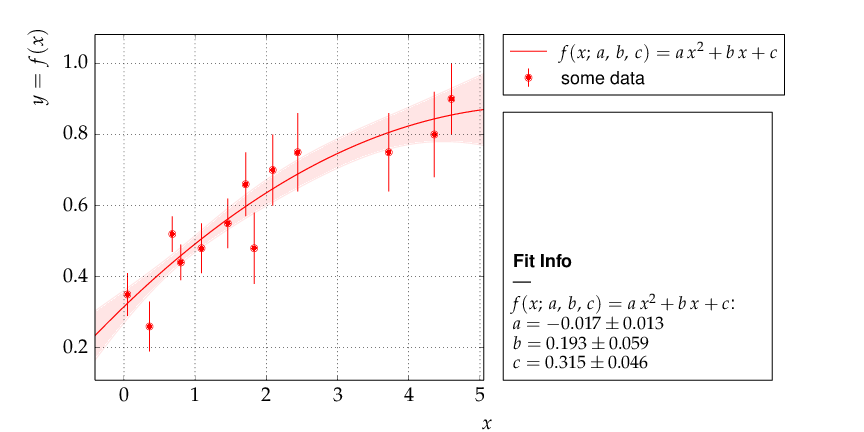
\includegraphics{kafe_example0.png}}
\caption{Example: \emph{Data points with one-dimensional error bars compared
to a quadratic model function with} \textbf{kafe}.}\end{figure}

More and advanced examples - like fitting different models
to one data set, comparison of different data sets with model
functions, averaging of correlated measurements or multi-parameter
fits - are provided as part of the \emph{kafe} distribution and are
described in the section \emph{Examples} below. They may serve as
a starting point for own applications.


\section{Installation}
\label{index:installation}
To install \emph{kafe}, unpack the archive \emph{kafe-\textless{}version\textgreater{}.tgz} , change to
the sub-directory  \emph{kafe-\textless{}versoin\textgreater{}/src/}  and follow the installation
instructions below.

1.) Install using \emph{pip}:
\begin{quote}

To install kafe using the \emph{Pip} installer
(\href{http://www.pip-installer.org/}{http://www.pip-installer.org/}), simply
run the helper script as root:
\begin{quote}

\code{./install.sh}
\end{quote}

If you don't have Pip installed, use:
\begin{quote}

\code{easy\_install pip}
\end{quote}

To remove kafe using pip, just run the helper script:
\begin{quote}

\code{./uninstall.sh}
\end{quote}
\end{quote}
\begin{enumerate}
\setcounter{enumi}{1}
\item {} 
Install using \emph{setuptools}:

Installing using Python's \emph{setup} tools works, but does not
provide a clean uninstall. Use this method if installing
with \emph{Pip} is not possible:
\begin{quote}

\code{python setup.py install}
\end{quote}

\end{enumerate}

Kafe needs a working version of the CERN data analysis framework \code{root},
freely available at  \href{http://root.cern.ch}{http://root.cern.ch}


\subsection{Dependencies}
\label{index:dependencies}
The recommended versions of external packages for kafe are as follows,
the version numbers in parentheses refer to the minimum requirements:

\begin{Verbatim}[commandchars=\\\{\}]
Python packages:
  * SciPy \textgreater{}= 0.12.0 (0.9.0), which includes
      - NumPy \textgreater{}= 1.7.1 (1.6.1) and
      - matplotlib \textgreater{}= 1.2.0 (1.1.1)

Other dependencies:
  * ROOT \textgreater{}= 5.34 (http://root.cern.ch)
  * Qt4 \textgreater{}= 4.8.5 {}`(could work with other versions){}`
  * PyQt \textgreater{}= 3.18.1 {}`(could work with other versions){}`
  * A LaTeX distribution {}`(tested with texlive){}`
\end{Verbatim}

Be sure that the version of \emph{ROOT} you use is compiled with \emph{PyROOT} support.
For \emph{Python} to see the \emph{PyROOT} bindings, the following environment variables
must be set correctly:

\begin{Verbatim}[commandchars=\\\{\}]
export ROOTSYS=\textless{}directory where ROOT is installed\textgreater{}
export LD\_LIBRARY\_PATH=\$\PYGZob{}LD\_LIBRARY\_PATH\PYGZcb{}:\$ROOTSYS/lib
export PYTHONPATH=\$ROOTSYS/lib:\$PYTHONPATH
\end{Verbatim}

For more info, refer to {[}\href{http://root.cern.ch/drupal/content/pyroot}{http://root.cern.ch/drupal/content/pyroot}{]}.

\emph{Qt} is needed because it is the supported interactive front-end for
\emph{matplotlib}. Other front-ends are not supported and can cause weird behaviour.

\emph{LaTeX} is used by \emph{matplotlib} for displaying labels and mathematical
expressions on graphs.


\chapter{Fit examples, utilities, tips and tricks}
\label{index:fit-examples-utilities-tips-and-tricks}
A wide range of applications of the kafe core and the usage of
the helper functions is exemplified here. All of them
are contained in the sub-directory \code{examples/} of the
cafe distribution and are intended to serve as a basis for
user projects.


\section{Example 1 - model comparison}
\label{index:example-1-model-comparison}
To decide whether a model is adequate to describe a given
set of data, typically several models have to be fit to the
same data. Here is the code for a comparison of a data set
to two models, namely a linear and an exponential function:

\begin{Verbatim}[commandchars=\\\{\}]
\# import everything we need from kafe
from kafe import *
\# additionally, import the two model functions we want to fit:
from kafe.function\_library import linear\_2par, exp\_2par

\#\#\#\#\#\#\#\#\#\#\#\#
\# Load the Dataset from the file
my\_dataset = Dataset(input\_file='dataset.dat', title="Example Dataset")
\#\#\# Create the Fits
my\_fits = [Fit(my\_dataset, exp\_2par),
         Fit(my\_dataset, linear\_2par)]
\#\#\# Do the Fits
for fit in my\_fits:
fit.do\_fit()
\#\#\# Create the plots, save and show output
my\_plot = Plot(my\_fits[0], my\_fits[1])
my\_plot.plot\_all(show\_data\_for=0) \# show data only once (it's the same data)
my\_plot.save('plot.pdf')
my\_plot.show()
\end{Verbatim}

The file \emph{dataset.dat} contains x and y data in the standard \emph{kafe} data
format, where values and errors (and optionally also correlation coefficients)
are given for each axis separately. \emph{\#} indicates a comment line, which
is ignored when reading the data:

\begin{Verbatim}[commandchars=\\\{\}]
\# axis 0: x
\# datapoints  uncor. err.
0.957426  3.0e-01
2.262212  3.0e-01
3.061167  3.0e-01
3.607280  3.0e-01
4.933100  3.0e-01
5.992332  3.0e-01
7.021234  3.0e-01
8.272489  3.0e-01
9.250817  3.0e-01
9.757758  3.0e-01

\# axis 1: y
\# datapoints  uncor. err.
1.672481  2.0e-01
1.743410  2.0e-01
1.805217  2.0e-01
2.147802  2.0e-01
2.679615  2.0e-01
3.110055  2.0e-01
3.723173  2.0e-01
4.430122  2.0e-01
4.944116  2.0e-01
5.698063  2.0e-01
\end{Verbatim}

The resulting output is shown below. As can be seen already
from the graph, the exponential model better describes the
data. The \(\chi\)² probability in the printed output shows, however,
that the linear model would be marginally acceptable as well:

\begin{Verbatim}[commandchars=\\\{\}]
linear\_2par
chi2prob 0.052
HYPTEST  accepted (CL 5\%)

exp\_2par
chi2prob 0.96
HYPTEST  accepted (CL 5\%)
\end{Verbatim}
\begin{figure}[htbp]
\centering
\capstart

\scalebox{1.000000}{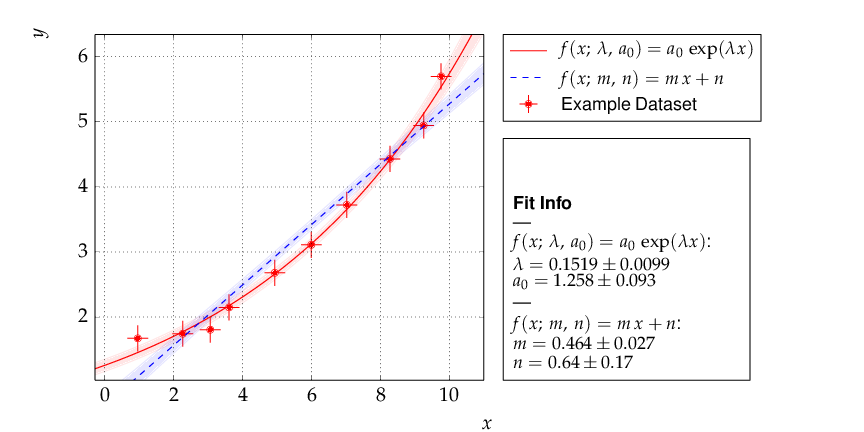
\includegraphics{kafe_example1.png}}
\caption{\emph{Output of example1 - compare two models}}\end{figure}


\section{Example 2 - two fits and models}
\label{index:example-2-two-fits-and-models}
Another typical use case consists of comparing two sets
of measurements and the models derived from them. This is
very similar to the previous example with minor
modifications:

\begin{Verbatim}[commandchars=\\\{\}]
\PYG{o}{.}\PYG{o}{.}\PYG{o}{.}

\PYG{c}{\PYGZsh{}\PYGZsh{}\PYGZsh{}\PYGZsh{}\PYGZsh{}\PYGZsh{}\PYGZsh{}\PYGZsh{}\PYGZsh{}\PYGZsh{}\PYGZsh{}\PYGZsh{}}
\PYG{c}{\PYGZsh{} Workflow \PYGZsh{}}
\PYG{c}{\PYGZsh{}\PYGZsh{}\PYGZsh{}\PYGZsh{}\PYGZsh{}\PYGZsh{}\PYGZsh{}\PYGZsh{}\PYGZsh{}\PYGZsh{}\PYGZsh{}\PYGZsh{}}
\PYG{c}{\PYGZsh{} Load two Datasets from files}
\PYG{n}{my\PYGZus{}datasets} \PYG{o}{=} \PYG{p}{[}\PYG{n}{Dataset}\PYG{p}{(}\PYG{n}{input\PYGZus{}file}\PYG{o}{=}\PYG{l+s}{\PYGZsq{}}\PYG{l+s}{dataset1.dat}\PYG{l+s}{\PYGZsq{}}\PYG{p}{,} \PYG{n}{title}\PYG{o}{=}\PYG{l+s}{\PYGZdq{}}\PYG{l+s}{Example Dataset 1}\PYG{l+s}{\PYGZdq{}}\PYG{p}{)}\PYG{p}{,}
             \PYG{n}{Dataset}\PYG{p}{(}\PYG{n}{input\PYGZus{}file}\PYG{o}{=}\PYG{l+s}{\PYGZsq{}}\PYG{l+s}{dataset2.dat}\PYG{l+s}{\PYGZsq{}}\PYG{p}{,} \PYG{n}{title}\PYG{o}{=}\PYG{l+s}{\PYGZdq{}}\PYG{l+s}{Example Dataset 2}\PYG{l+s}{\PYGZdq{}}\PYG{p}{)}\PYG{p}{]}
\PYG{c}{\PYGZsh{} Create the Fits}
\PYG{o}{.}\PYG{o}{.}\PYG{o}{.}
\PYG{c}{\PYGZsh{} Do the Fits}
\PYG{o}{.}\PYG{o}{.}\PYG{o}{.}
\PYG{c}{\PYGZsh{} Create the plots}
\PYG{n}{my\PYGZus{}plot}\PYG{o}{.}\PYG{n}{plot\PYGZus{}all}\PYG{p}{(}\PYG{p}{)} \PYG{c}{\PYGZsh{} this time withouth argument, i.e. show everything}
\PYG{o}{.}\PYG{o}{.}\PYG{o}{.}
\end{Verbatim}

This results in the following output:
\begin{figure}[htbp]
\centering
\capstart

\scalebox{1.000000}{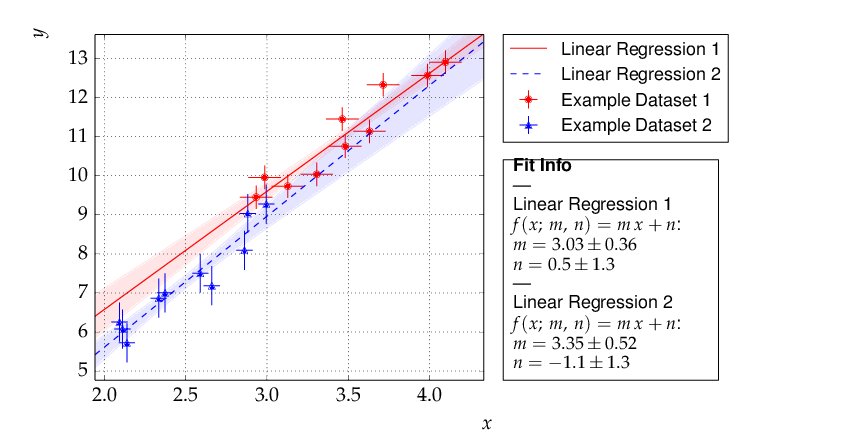
\includegraphics{kafe_example2.png}}
\caption{\emph{Output of example2 - comparison of two linear fits.}}\end{figure}

Although the parameters extracted from the two data sets agree within
errors, the uncertainty bands of the two functions do not overlap
in the region where the data of Dataset 2 are located, so the data
are most probably incompatible with the assumption of an underlying
single linear model.


\section{Example 3 - properties of a Gauss curve}
\label{index:example-3-properties-of-a-gauss-curve}
This example creates a dummy \code{Dataset} object whose points lie exactly
on a Gaussian curve. The \code{Fit} will then converge toward that very same
Gaussian. When plotting, the data points used to ``support'' the curve
can be omitted.

This example shows how to access the \emph{kafe} plot objects
to annotate plots with \emph{matplotlib} functionality.
\begin{figure}[htbp]
\centering
\capstart

\scalebox{1.000000}{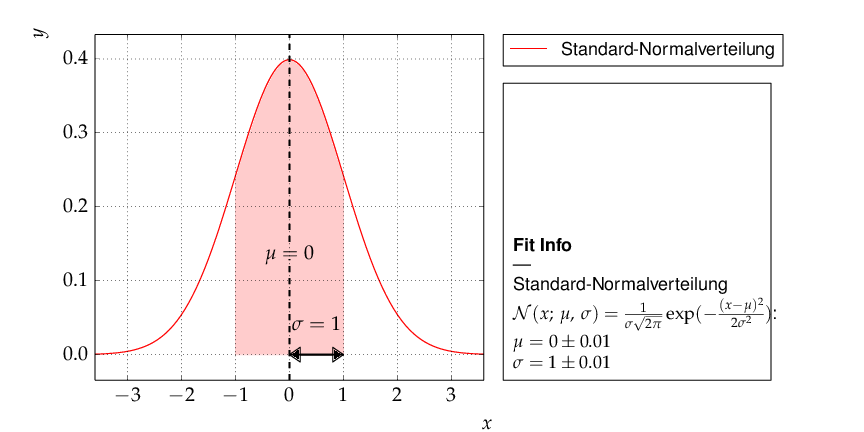
\includegraphics{kafe_example3.png}}
\caption{\emph{Output of example 3 - properties of a Gauss curve.}}\end{figure}


\section{Example 4 - average of correlated measurements}
\label{index:example-4-average-of-correlated-measurements}
The average of a set of measurements can be considered as a fit
of a constant to a set of input data. This example illustrates
how correlated errors are handled in \emph{kafe}.
Measurements can have a common error, which may be absolute
or relative, i. e. depend on the input value.  In more complicated
cases the full covariance matrix must be constructed.

\emph{kafe} has a helper function, \code{build\_dataset} in module \code{fit},
which aids in setting up the covariance matrix and transforming
the input to the default format used by the \code{Dataset} and \code{Fit}
classes. Two further helper functions in module \code{file\_tools}
aid in reading the appropriate information from data files.
\begin{enumerate}
\item {} 
The function  \code{parse\_column\_data} reads the input values and their
independent errors from one file, and optionally covariance
matrices for the x and y axes from additional files. The field ordering
is defined by a control string.

\item {} 
Another helper function, \code{buildDataset\_fromFile}, specifies
input values or blocks of input data from a single file with
keywords.

\end{enumerate}

The second version needs only very minimal additional user
code, as illustrated here:

\begin{Verbatim}[commandchars=\\\{\}]
\PYG{k+kn}{from} \PYG{n+nn}{kafe} \PYG{k+kn}{import} \PYG{o}{*}
\PYG{k+kn}{from} \PYG{n+nn}{kafe.function\PYGZus{}library} \PYG{k+kn}{import} \PYG{n}{constant\PYGZus{}1par}
\PYG{k+kn}{from} \PYG{n+nn}{kafe.file\PYGZus{}tools} \PYG{k+kn}{import} \PYG{n}{buildDataset\PYGZus{}fromFile}
\PYG{c}{\PYGZsh{}}
\PYG{c}{\PYGZsh{} \PYGZhy{}\PYGZhy{}\PYGZhy{}\PYGZhy{}\PYGZhy{}\PYGZhy{}\PYGZhy{}\PYGZhy{}\PYGZhy{}\PYGZhy{}\PYGZhy{}\PYGZhy{}\PYGZhy{}\PYGZhy{}\PYGZhy{}\PYGZhy{}\PYGZhy{}\PYGZhy{}\PYGZhy{}\PYGZhy{}\PYGZhy{}\PYGZhy{}\PYGZhy{}\PYGZhy{}\PYGZhy{}\PYGZhy{}\PYGZhy{}\PYGZhy{}\PYGZhy{}\PYGZhy{}\PYGZhy{}\PYGZhy{}\PYGZhy{}\PYGZhy{}\PYGZhy{}\PYGZhy{}\PYGZhy{}\PYGZhy{}\PYGZhy{}\PYGZhy{}\PYGZhy{}\PYGZhy{}\PYGZhy{}\PYGZhy{}\PYGZhy{}\PYGZhy{}\PYGZhy{}\PYGZhy{}\PYGZhy{}\PYGZhy{}\PYGZhy{}\PYGZhy{}\PYGZhy{}\PYGZhy{}\PYGZhy{}\PYGZhy{}\PYGZhy{}}
\PYG{n}{fname}\PYG{o}{=}\PYG{l+s}{\PYGZsq{}}\PYG{l+s}{WData.dat}\PYG{l+s}{\PYGZsq{}}
\PYG{n}{curDataset}\PYG{o}{=}\PYG{n}{buildDataset\PYGZus{}fromFile}\PYG{p}{(}\PYG{n}{fname}\PYG{p}{)} \PYG{c}{\PYGZsh{} Dataset from input file}
\PYG{n}{curFit}\PYG{o}{=}\PYG{n}{Fit}\PYG{p}{(}\PYG{n}{curDataset}\PYG{p}{,} \PYG{n}{constant\PYGZus{}1par}\PYG{p}{)}   \PYG{c}{\PYGZsh{} set up the fit object}
\PYG{n}{curFit}\PYG{o}{.}\PYG{n}{do\PYGZus{}fit}\PYG{p}{(}\PYG{p}{)}

\PYG{n}{myPlot}\PYG{o}{=}\PYG{n}{Plot}\PYG{p}{(}\PYG{n}{curFit}\PYG{p}{)}
\PYG{n}{myPlot}\PYG{o}{.}\PYG{n}{plot\PYGZus{}all}\PYG{p}{(}\PYG{p}{)}
\PYG{n}{myPlot}\PYG{o}{.}\PYG{n}{save}\PYG{p}{(}\PYG{l+s}{\PYGZdq{}}\PYG{l+s}{plot.pdf}\PYG{l+s}{\PYGZdq{}}\PYG{p}{)}
\PYG{n}{myPlot}\PYG{o}{.}\PYG{n}{show}\PYG{p}{(}\PYG{p}{)}
\end{Verbatim}

The input file is necessarily more complicated, but holds
the full information on the data set in one place. Refer to
the documentation of the module \code{parse\_general\_inputfile}
in module \code{file\_tools} for a full description of the
presently implemented keywords. The input file for the
averaging example is here:

\begin{Verbatim}[commandchars=\\\{\}]
\# Measurements of W boson mass (combined LEP2, 2013)
\# --------------------------------------------------
\# example to use parse\_general\_inputfile from kafe;
\#  covariance matrix build from common errors
\# --
\#  Meta data for plotting
*TITLE measurements of the W boson mass
*xLabel number of measurement
*yLabel \$m\_\PYGZbs{}matrhm\PYGZob{}W\PYGZcb{}\$
*yUnit GeV/\$c\textasciicircum{}2\$

\# x data need not be given for averaging

\# ------------------------------------------------------------
\#  Measurements of W mass by ALEPH, DELPI, L3 and OPAL
\#                              from from LEP2 Report Feb. 2013
\#  common errors within channels
\#                     2q2l: 0.021 GeV,
\#                       4q: 0.044 GeV,
\#     and between channels: 0.025 GeV
\# ------------------------------------------------------------

*yData\_SCOV
\# W\_mass  err     syst    sqrt of the off-diagonal
\# 2q2l channel                           elements of the
80.429  0.055   0.021          \#         covariance matrix
80.339  0.073   0.021   0.021
80.217  0.068   0.021   0.021 0.021
80.449  0.058   0.021   0.021 0.021 0.021
\# 4q  channel
80.477  0.069   0.044   0.025 0.025 0.025 0.025 0.044
80.310  0.091   0.044   0.025 0.025 0.025 0.025 0.044 0.044
80.324  0.078   0.044   0.025 0.025 0.025 0.025 0.044 0.044 0.044
80.353  0.068   0.044   0.025 0.025 0.025 0.025 0.044 0.044 0.044 0.044
\end{Verbatim}


\section{Example 5 - multi-parameter fit (damped oscillation)}
\label{index:example-5-multi-parameter-fit-damped-oscillation}
This example shows the fitting of a more complicated model function
to data collected from a damped harmonic oscillator. In such
non-linear fits, stetting the initial values is sometimes crucial
to let the fit converge at the global minimum. The \code{Fit} object
provides the method \code{set\_parameters} for this purpose. As the
fit function for this problem is not a standard one, it is defined
explicitly making use of the decorator functions available in \emph{kafe}
to provide nice type setting of the parameters. This time, the
function \code{parse\_colmn\_data} is used to read the input,
which is given as separate columns with the fields
\begin{quote}

\code{\textless{}time\textgreater{}  \textless{}Amplitude\textgreater{}    \textless{}error on time\textgreater{}   \textless{}error on Amplitude\textgreater{}}
\end{quote}

Here is the example code:

\begin{Verbatim}[commandchars=\\\{\}]
\PYG{o}{.}\PYG{o}{.}\PYG{o}{.}
\PYG{k+kn}{from} \PYG{n+nn}{kafe} \PYG{k+kn}{import} \PYG{o}{*}
\PYG{k+kn}{from} \PYG{n+nn}{numpy} \PYG{k+kn}{import} \PYG{n}{exp}\PYG{p}{,} \PYG{n}{cos}
\PYG{c}{\PYGZsh{} Model function definition \PYGZsh{}}
\PYG{c}{\PYGZsh{} \PYGZhy{}\PYGZhy{}\PYGZhy{}\PYGZhy{}\PYGZhy{}\PYGZhy{}\PYGZhy{}\PYGZhy{}\PYGZhy{}\PYGZhy{}\PYGZhy{}\PYGZhy{}\PYGZhy{}\PYGZhy{}\PYGZhy{}\PYGZhy{}\PYGZhy{}\PYGZhy{}\PYGZhy{}\PYGZhy{}\PYGZhy{}\PYGZhy{}\PYGZhy{}\PYGZhy{}\PYGZhy{}\PYGZhy{}\PYGZhy{}}
\PYG{c}{\PYGZsh{} Set an ASCII expression for this function}
\PYG{n+nd}{@ASCII}\PYG{p}{(}\PYG{n}{x\PYGZus{}name}\PYG{o}{=}\PYG{l+s}{\PYGZdq{}}\PYG{l+s}{t}\PYG{l+s}{\PYGZdq{}}\PYG{p}{,} \PYG{n}{expression}\PYG{o}{=}\PYG{l+s}{\PYGZdq{}}\PYG{l+s}{A0*exp(\PYGZhy{}t/tau)*cos(omega*t+phi)}\PYG{l+s}{\PYGZdq{}}\PYG{p}{)}
\PYG{c}{\PYGZsh{} Set some LaTeX\PYGZhy{}related parameters for this function}
\PYG{n+nd}{@LaTeX}\PYG{p}{(}\PYG{n}{name}\PYG{o}{=}\PYG{l+s}{\PYGZsq{}}\PYG{l+s}{A}\PYG{l+s}{\PYGZsq{}}\PYG{p}{,} \PYG{n}{x\PYGZus{}name}\PYG{o}{=}\PYG{l+s}{\PYGZdq{}}\PYG{l+s}{t}\PYG{l+s}{\PYGZdq{}}\PYG{p}{,}
       \PYG{n}{parameter\PYGZus{}names}\PYG{o}{=}\PYG{p}{(}\PYG{l+s}{\PYGZsq{}}\PYG{l+s}{a\PYGZus{}0}\PYG{l+s}{\PYGZsq{}}\PYG{p}{,} \PYG{l+s}{\PYGZsq{}}\PYG{l+s+se}{\PYGZbs{}\PYGZbs{}}\PYG{l+s}{tau\PYGZob{}\PYGZcb{}}\PYG{l+s}{\PYGZsq{}}\PYG{p}{,} \PYG{l+s}{\PYGZsq{}}\PYG{l+s+se}{\PYGZbs{}\PYGZbs{}}\PYG{l+s}{omega\PYGZob{}\PYGZcb{}}\PYG{l+s}{\PYGZsq{}}\PYG{p}{,} \PYG{l+s}{\PYGZsq{}}\PYG{l+s+se}{\PYGZbs{}\PYGZbs{}}\PYG{l+s}{varphi\PYGZob{}\PYGZcb{}}\PYG{l+s}{\PYGZsq{}}\PYG{p}{)}\PYG{p}{,}
       \PYG{n}{expression}\PYG{o}{=}\PYG{l+s}{\PYGZdq{}}\PYG{l+s}{a\PYGZus{}0}\PYG{l+s+se}{\PYGZbs{}\PYGZbs{}}\PYG{l+s}{,}\PYG{l+s+se}{\PYGZbs{}\PYGZbs{}}\PYG{l+s}{exp(\PYGZhy{}}\PYG{l+s+se}{\PYGZbs{}\PYGZbs{}}\PYG{l+s}{frac\PYGZob{}t\PYGZcb{}\PYGZob{}}\PYG{l+s+se}{\PYGZbs{}\PYGZbs{}}\PYG{l+s}{tau\PYGZcb{})}\PYG{l+s}{\PYGZbs{}}\PYG{l+s}{,}\PYG{l+s}{\PYGZdq{}}
                  \PYG{l+s}{\PYGZdq{}}\PYG{l+s}{\PYGZbs{}}\PYG{l+s}{cos(}\PYG{l+s+se}{\PYGZbs{}\PYGZbs{}}\PYG{l+s}{omega\PYGZob{}\PYGZcb{}}\PYG{l+s+se}{\PYGZbs{}\PYGZbs{}}\PYG{l+s}{,t+}\PYG{l+s+se}{\PYGZbs{}\PYGZbs{}}\PYG{l+s}{varphi\PYGZob{}\PYGZcb{})}\PYG{l+s}{\PYGZdq{}}\PYG{p}{)}
\PYG{n+nd}{@FitFunction}
\PYG{k}{def} \PYG{n+nf}{damped\PYGZus{}oscillator}\PYG{p}{(}\PYG{n}{t}\PYG{p}{,} \PYG{n}{a0}\PYG{o}{=}\PYG{l+m+mi}{1}\PYG{p}{,} \PYG{n}{tau}\PYG{o}{=}\PYG{l+m+mi}{1}\PYG{p}{,} \PYG{n}{omega}\PYG{o}{=}\PYG{l+m+mi}{1}\PYG{p}{,} \PYG{n}{phi}\PYG{o}{=}\PYG{l+m+mi}{0}\PYG{p}{)}\PYG{p}{:}
    \PYG{k}{return} \PYG{n}{a0} \PYG{o}{*} \PYG{n}{exp}\PYG{p}{(}\PYG{o}{\PYGZhy{}}\PYG{n}{t}\PYG{o}{/}\PYG{n}{tau}\PYG{p}{)} \PYG{o}{*} \PYG{n}{cos}\PYG{p}{(}\PYG{n}{omega}\PYG{o}{*}\PYG{n}{t} \PYG{o}{+} \PYG{n}{phi}\PYG{p}{)}

\PYG{c}{\PYGZsh{} \PYGZhy{}\PYGZhy{}\PYGZhy{}\PYGZhy{} Workflow \PYGZsh{}}
\PYG{c}{\PYGZsh{} load the experimental data from a file}
\PYG{n}{my\PYGZus{}dataset} \PYG{o}{=} \PYG{n}{parse\PYGZus{}column\PYGZus{}data}\PYG{p}{(}\PYG{l+s}{\PYGZsq{}}\PYG{l+s}{damped\PYGZus{}oscillation.dat}\PYG{l+s}{\PYGZsq{}}\PYG{p}{,}
    \PYG{n}{field\PYGZus{}order}\PYG{o}{=}\PYG{l+s}{\PYGZdq{}}\PYG{l+s}{x,y,xabserr,yabserr}\PYG{l+s}{\PYGZdq{}}\PYG{p}{,} \PYG{n}{title}\PYG{o}{=}\PYG{l+s}{\PYGZdq{}}\PYG{l+s}{Damped Oscillator}\PYG{l+s}{\PYGZdq{}}\PYG{p}{,}
    \PYG{n}{axis\PYGZus{}labels}\PYG{o}{=}\PYG{p}{[}\PYG{l+s}{\PYGZsq{}}\PYG{l+s}{Time t}\PYG{l+s}{\PYGZsq{}}\PYG{p}{,} \PYG{l+s}{\PYGZsq{}}\PYG{l+s}{Amplitude}\PYG{l+s}{\PYGZsq{}}\PYG{p}{]}\PYG{p}{)}
\PYG{c}{\PYGZsh{} \PYGZhy{}\PYGZhy{}\PYGZhy{} Create the Fit}
\PYG{n}{my\PYGZus{}fit} \PYG{o}{=} \PYG{n}{Fit}\PYG{p}{(}\PYG{n}{my\PYGZus{}dataset}\PYG{p}{,} \PYG{n}{damped\PYGZus{}oscillator}\PYG{p}{)}
\PYG{c}{\PYGZsh{} Set the initial values for the fit:}
\PYG{c}{\PYGZsh{}                      a\PYGZus{}0 tau omega phi}
\PYG{n}{my\PYGZus{}fit}\PYG{o}{.}\PYG{n}{set\PYGZus{}parameters}\PYG{p}{(}\PYG{p}{(}\PYG{l+m+mf}{1.}\PYG{p}{,} \PYG{l+m+mf}{3.}\PYG{p}{,} \PYG{l+m+mf}{6.28}\PYG{p}{,} \PYG{l+m+mf}{0.}\PYG{p}{)}\PYG{p}{)}
\PYG{n}{my\PYGZus{}fit}\PYG{o}{.}\PYG{n}{do\PYGZus{}fit}\PYG{p}{(}\PYG{p}{)}
\PYG{c}{\PYGZsh{} \PYGZhy{}\PYGZhy{}\PYGZhy{} Create and output the plots}
\PYG{n}{my\PYGZus{}plot} \PYG{o}{=} \PYG{n}{Plot}\PYG{p}{(}\PYG{n}{my\PYGZus{}fit}\PYG{p}{)}
\PYG{n}{my\PYGZus{}plot}\PYG{o}{.}\PYG{n}{plot\PYGZus{}all}\PYG{p}{(}\PYG{p}{)}
\PYG{n}{my\PYGZus{}plot}\PYG{o}{.}\PYG{n}{save}\PYG{p}{(}\PYG{l+s}{\PYGZsq{}}\PYG{l+s}{plot.pdf}\PYG{l+s}{\PYGZsq{}}\PYG{p}{)}
\PYG{n}{my\PYGZus{}plot}\PYG{o}{.}\PYG{n}{show}\PYG{p}{(}\PYG{p}{)}
\end{Verbatim}
\begin{figure}[htbp]
\centering
\capstart

\scalebox{1.000000}{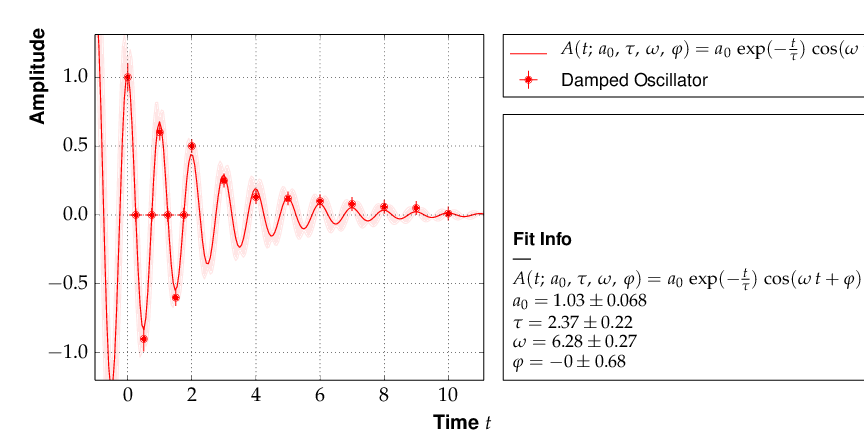
\includegraphics{kafe_example5.png}}
\caption{\emph{Example 5 - fit of the time dependence of the amplitude of a damped harmonic oscillator.}}\end{figure}


\section{Example 6 - another multi-parameter fit}
\label{index:example-6-another-multi-parameter-fit}
This example is not much different from the previous one, except that
the fit function, a standard fourth-degree polynomial from the module
\code{function\_library}, is modified to reflect the names of the problem
given, and \emph{matplotlib} functionality is used to influence the
ouput of the plot, e.g. axis names and linear or logarithmic scale.

It is also shown how to circumvent a problem that
often arises when errors depend on the measured values.
For a counting rate, the (statistical) error is typically estimated
as the square root of the (observed) number of entries in each bin.
For large numbers of entries, this is not a problem,
but for small numbers, the correlation between the observed
number of entries and the error derived from it leads to a
bias when fitting functions to the data. This problem can be
avoided by iterating the fit procedure:

In a pre-fit, a first approximation of the model function is
determined, which is then used to calculate
the expected errors, and the origial errors are
replaced before performing the final fit. Note that the numbers
of entries in the bins must be sufficiently large to justify
a replacement of the (asymmetric) Poission uncertainties by
the symmetric uncertainties implied by the \(\chi\)²-method.

The implementation of this  procedure needs accesses some
more fundamental methods of the \emph{Dataset}, \emph{Fit} and
\emph{FitFunction} classes. The code shown below demonstrates
how this can be done with \emph{kafe}, using some of its lower-level,
internal interfaces:

\begin{Verbatim}[commandchars=\\\{\}]
\PYG{k+kn}{from} \PYG{n+nn}{kafe.function\PYGZus{}library} \PYG{k+kn}{import} \PYG{n}{poly4}
\PYG{c}{\PYGZsh{} modify function\PYGZsq{}s independent variable name to reflect its nature:}
\PYG{n}{poly4}\PYG{o}{.}\PYG{n}{x\PYGZus{}name} \PYG{o}{=} \PYG{l+s}{\PYGZsq{}}\PYG{l+s}{x=cos(t)}\PYG{l+s}{\PYGZsq{}}
\PYG{n}{poly4}\PYG{o}{.}\PYG{n}{latex\PYGZus{}x\PYGZus{}name} \PYG{o}{=} \PYG{l+s}{\PYGZsq{}}\PYG{l+s}{x=}\PYG{l+s+se}{\PYGZbs{}\PYGZbs{}}\PYG{l+s}{cos(}\PYG{l+s+se}{\PYGZbs{}\PYGZbs{}}\PYG{l+s}{theta)}\PYG{l+s}{\PYGZsq{}}
\PYG{o}{.}\PYG{o}{.}\PYG{o}{.}

\PYG{c}{\PYGZsh{} Set the axis labels appropriately}
\PYG{n}{my\PYGZus{}plot}\PYG{o}{.}\PYG{n}{axis\PYGZus{}labels} \PYG{o}{=} \PYG{p}{[}\PYG{l+s}{\PYGZsq{}}\PYG{l+s}{\PYGZdl{}}\PYG{l+s+se}{\PYGZbs{}\PYGZbs{}}\PYG{l+s}{cos(}\PYG{l+s+se}{\PYGZbs{}\PYGZbs{}}\PYG{l+s}{theta)\PYGZdl{}}\PYG{l+s}{\PYGZsq{}}\PYG{p}{,} \PYG{l+s}{\PYGZsq{}}\PYG{l+s}{counting rate}\PYG{l+s}{\PYGZsq{}}\PYG{p}{]}
\PYG{o}{.}\PYG{o}{.}\PYG{o}{.}
\PYG{c}{\PYGZsh{} load the experimental data from a file}
\PYG{n}{my\PYGZus{}dataset} \PYG{o}{=} \PYG{n}{parse\PYGZus{}column\PYGZus{}data}\PYG{p}{(}
  \PYG{l+s}{\PYGZsq{}}\PYG{l+s}{counting\PYGZus{}rate.dat}\PYG{l+s}{\PYGZsq{}}\PYG{p}{,}
  \PYG{n}{field\PYGZus{}order}\PYG{o}{=}\PYG{l+s}{\PYGZdq{}}\PYG{l+s}{x,y,yabserr}\PYG{l+s}{\PYGZdq{}}\PYG{p}{,}
  \PYG{n}{title}\PYG{o}{=}\PYG{l+s}{\PYGZdq{}}\PYG{l+s}{Counting Rate per Angle}\PYG{l+s}{\PYGZdq{}}\PYG{p}{)}

\PYG{c}{\PYGZsh{}\PYGZsh{}\PYGZsh{} pre\PYGZhy{}fit}
\PYG{c}{\PYGZsh{} error for bins with zero contents is set to 1.}
\PYG{n}{covmat} \PYG{o}{=} \PYG{n}{my\PYGZus{}dataset}\PYG{o}{.}\PYG{n}{get\PYGZus{}cov\PYGZus{}mat}\PYG{p}{(}\PYG{l+s}{\PYGZsq{}}\PYG{l+s}{y}\PYG{l+s}{\PYGZsq{}}\PYG{p}{)}
\PYG{k}{for} \PYG{n}{i} \PYG{o+ow}{in} \PYG{n+nb}{range}\PYG{p}{(}\PYG{l+m+mi}{0}\PYG{p}{,} \PYG{n+nb}{len}\PYG{p}{(}\PYG{n}{covmat}\PYG{p}{)}\PYG{p}{)}\PYG{p}{:}
    \PYG{k}{if} \PYG{n}{covmat}\PYG{p}{[}\PYG{n}{i}\PYG{p}{,} \PYG{n}{i}\PYG{p}{]}\PYG{o}{==}\PYG{l+m+mf}{0.}\PYG{p}{:}
        \PYG{n}{covmat}\PYG{p}{[}\PYG{n}{i}\PYG{p}{,} \PYG{n}{i}\PYG{p}{]}\PYG{o}{=}\PYG{l+m+mf}{1.}
\PYG{n}{my\PYGZus{}dataset}\PYG{o}{.}\PYG{n}{set\PYGZus{}cov\PYGZus{}mat}\PYG{p}{(}\PYG{l+s}{\PYGZsq{}}\PYG{l+s}{y}\PYG{l+s}{\PYGZsq{}}\PYG{p}{,} \PYG{n}{covmat}\PYG{p}{)} \PYG{c}{\PYGZsh{} write it back}

\PYG{c}{\PYGZsh{} Create the Fit}
\PYG{n}{my\PYGZus{}fit} \PYG{o}{=} \PYG{n}{Fit}\PYG{p}{(}\PYG{n}{my\PYGZus{}dataset}\PYG{p}{,} \PYG{n}{poly4}\PYG{p}{)}
\PYG{c}{\PYGZsh{}            fit\PYGZus{}label=\PYGZdq{}Linear Regression \PYGZdq{} + dataset.data\PYGZus{}label[\PYGZhy{}1])}

\PYG{c}{\PYGZsh{} perform an initial fit with temporary errors (minimial output)}
\PYG{n}{my\PYGZus{}fit}\PYG{o}{.}\PYG{n}{call\PYGZus{}minimizer}\PYG{p}{(}\PYG{n}{final\PYGZus{}fit}\PYG{o}{=}\PYG{n+nb+bp}{False}\PYG{p}{,} \PYG{n}{verbose}\PYG{o}{=}\PYG{n+nb+bp}{False}\PYG{p}{)}

\PYG{c}{\PYGZsh{} set errors using model at pre\PYGZhy{}fit parameter values:}
\PYG{c}{\PYGZsh{}       sigma\PYGZus{}i\PYGZca{}2=cov[i,i]=n(x\PYGZus{}i)}
\PYG{n}{fdata} \PYG{o}{=} \PYG{n}{my\PYGZus{}fit}\PYG{o}{.}\PYG{n}{fit\PYGZus{}function}\PYG{o}{.}\PYG{n}{evaluate}\PYG{p}{(}\PYG{n}{my\PYGZus{}fit}\PYG{o}{.}\PYG{n}{xdata}\PYG{p}{,}
                                   \PYG{n}{my\PYGZus{}fit}\PYG{o}{.}\PYG{n}{current\PYGZus{}parameter\PYGZus{}values}\PYG{p}{)}
\PYG{n}{np}\PYG{o}{.}\PYG{n}{fill\PYGZus{}diagonal}\PYG{p}{(}\PYG{n}{covmat}\PYG{p}{,} \PYG{n}{fdata}\PYG{p}{)}
\PYG{n}{my\PYGZus{}fit}\PYG{o}{.}\PYG{n}{current\PYGZus{}cov\PYGZus{}mat} \PYG{o}{=} \PYG{n}{covmat}  \PYG{c}{\PYGZsh{} write new covariance matrix}
\PYG{c}{\PYGZsh{}\PYGZsh{}\PYGZsh{} end pre\PYGZhy{}fit \PYGZhy{} rest ist as usual}
\PYG{n}{my\PYGZus{}fit}\PYG{o}{.}\PYG{n}{do\PYGZus{}fit}\PYG{p}{(}\PYG{p}{)}
\PYG{c}{\PYGZsh{} Create the plots and \PYGZhy{}\PYGZhy{}}
\PYG{n}{my\PYGZus{}plot} \PYG{o}{=} \PYG{n}{Plot}\PYG{p}{(}\PYG{n}{my\PYGZus{}fit}\PYG{p}{)}
\PYG{c}{\PYGZsh{} \PYGZhy{}\PYGZhy{} set the axis labels}
\PYG{n}{my\PYGZus{}plot}\PYG{o}{.}\PYG{n}{axis\PYGZus{}labels} \PYG{o}{=} \PYG{p}{[}\PYG{l+s}{\PYGZsq{}}\PYG{l+s}{\PYGZdl{}}\PYG{l+s+se}{\PYGZbs{}\PYGZbs{}}\PYG{l+s}{cos(}\PYG{l+s+se}{\PYGZbs{}\PYGZbs{}}\PYG{l+s}{theta)\PYGZdl{}}\PYG{l+s}{\PYGZsq{}}\PYG{p}{,} \PYG{l+s}{\PYGZsq{}}\PYG{l+s}{counting rate}\PYG{l+s}{\PYGZsq{}}\PYG{p}{]}
\PYG{c}{\PYGZsh{} \PYGZhy{}\PYGZhy{} set scale linear / log}
\PYG{n}{my\PYGZus{}plot}\PYG{o}{.}\PYG{n}{axes}\PYG{o}{.}\PYG{n}{set\PYGZus{}yscale}\PYG{p}{(}\PYG{l+s}{\PYGZsq{}}\PYG{l+s}{linear}\PYG{l+s}{\PYGZsq{}}\PYG{p}{)}
\PYG{o}{.}\PYG{o}{.}\PYG{o}{.}
\end{Verbatim}

This is the resulting output:
\begin{figure}[htbp]
\centering
\capstart

\scalebox{1.000000}{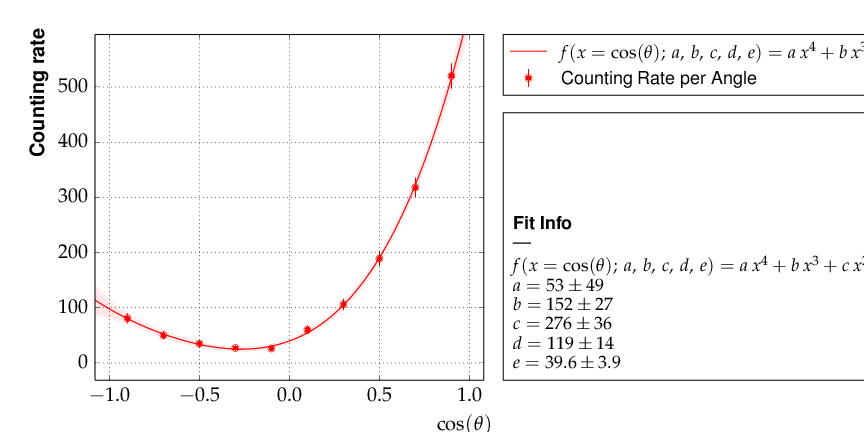
\includegraphics{kafe_example6.png}}
\caption{\emph{Output of example 6 - counting rate.}}\end{figure}


\section{Example 7 - non-linear multi-parameter fit}
\label{index:example-7-non-linear-multi-parameter-fit}
Again, not much new in this example, except that the
model is now very non-linear, the intensity distribution
of light after passing through a double-slit. The
non-standard model definition again makes use of the
decorator mechanism to provide nice output - the decorators
(expressions beginning with `@') can safely be omitted if \emph{LaTeX}
output is not needed. Setting of appropriate initial
conditions is absolutely mandatory for this example,
because there  exist many local minima of the \(\chi\)² function.

Another problem becomes obvious when carefully inspecting
the fit function definition: only two of the three parameters g,
b or k can be determined, and therefore one must be kept fixed,
or an external constraint must be applied.
Failing to do so will result in large, correlated errors
on the parameters g, b and k as an indication of the problem.

Fixing parameters of a model function is achieved by the method
\code{fix\_parameters()}, and a constraint within a given uncertainty
is achieved by the method \code{constrain\_parameters()}
of the \code{Fit} class.

Here are the interesting pieces of code:

\begin{Verbatim}[commandchars=\\\{\}]
\PYG{o}{.}\PYG{o}{.}\PYG{o}{.}
\PYG{c}{\PYGZsh{} Model function definition \PYGZsh{}}
\PYG{c}{\PYGZsh{} Set an ASCII expression for this function}
\PYG{n+nd}{@ASCII}\PYG{p}{(}\PYG{n}{x\PYGZus{}name}\PYG{o}{=}\PYG{l+s}{\PYGZdq{}}\PYG{l+s}{x}\PYG{l+s}{\PYGZdq{}}\PYG{p}{,} \PYG{n}{expression}\PYG{o}{=}\PYG{l+s}{\PYGZdq{}}\PYG{l+s}{I0*(sin(k/2*b*sin(x))/(k/2*b*sin(x))}\PYG{l+s}{\PYGZdq{}}
                              \PYG{l+s}{\PYGZdq{}}\PYG{l+s}{*cos(k/2*g*sin(x)))\PYGZca{}2}\PYG{l+s}{\PYGZdq{}}\PYG{p}{)}
\PYG{c}{\PYGZsh{} Set some LaTeX\PYGZhy{}related parameters for this function}
\PYG{n+nd}{@LaTeX}\PYG{p}{(}\PYG{n}{name}\PYG{o}{=}\PYG{l+s}{\PYGZsq{}}\PYG{l+s}{I}\PYG{l+s}{\PYGZsq{}}\PYG{p}{,} \PYG{n}{x\PYGZus{}name}\PYG{o}{=}\PYG{l+s}{\PYGZdq{}}\PYG{l+s+se}{\PYGZbs{}\PYGZbs{}}\PYG{l+s}{alpha\PYGZob{}\PYGZcb{}}\PYG{l+s}{\PYGZdq{}}\PYG{p}{,}
       \PYG{n}{parameter\PYGZus{}names}\PYG{o}{=}\PYG{p}{(}\PYG{l+s}{\PYGZsq{}}\PYG{l+s}{I\PYGZus{}0}\PYG{l+s}{\PYGZsq{}}\PYG{p}{,} \PYG{l+s}{\PYGZsq{}}\PYG{l+s}{b}\PYG{l+s}{\PYGZsq{}}\PYG{p}{,} \PYG{l+s}{\PYGZsq{}}\PYG{l+s}{g}\PYG{l+s}{\PYGZsq{}}\PYG{p}{,} \PYG{l+s}{\PYGZsq{}}\PYG{l+s}{k}\PYG{l+s}{\PYGZsq{}}\PYG{p}{)}\PYG{p}{,}
       \PYG{n}{expression}\PYG{o}{=}\PYG{l+s}{\PYGZdq{}}\PYG{l+s}{I\PYGZus{}0}\PYG{l+s+se}{\PYGZbs{}\PYGZbs{}}\PYG{l+s}{,}\PYG{l+s+se}{\PYGZbs{}\PYGZbs{}}\PYG{l+s}{left(}\PYG{l+s+se}{\PYGZbs{}\PYGZbs{}}\PYG{l+s}{frac\PYGZob{}}\PYG{l+s+se}{\PYGZbs{}\PYGZbs{}}\PYG{l+s}{sin(}\PYG{l+s+se}{\PYGZbs{}\PYGZbs{}}\PYG{l+s}{frac\PYGZob{}k\PYGZcb{}\PYGZob{}2\PYGZcb{}}\PYG{l+s+se}{\PYGZbs{}\PYGZbs{}}\PYG{l+s}{,b}\PYG{l+s+se}{\PYGZbs{}\PYGZbs{}}\PYG{l+s}{,}\PYG{l+s+se}{\PYGZbs{}\PYGZbs{}}\PYG{l+s}{sin\PYGZob{}}\PYG{l+s+se}{\PYGZbs{}\PYGZbs{}}\PYG{l+s}{alpha\PYGZcb{})\PYGZcb{}}\PYG{l+s}{\PYGZdq{}}
                  \PYG{l+s}{\PYGZdq{}}\PYG{l+s}{\PYGZob{}}\PYG{l+s+se}{\PYGZbs{}\PYGZbs{}}\PYG{l+s}{frac\PYGZob{}k\PYGZcb{}\PYGZob{}2\PYGZcb{}}\PYG{l+s+se}{\PYGZbs{}\PYGZbs{}}\PYG{l+s}{,b}\PYG{l+s+se}{\PYGZbs{}\PYGZbs{}}\PYG{l+s}{,}\PYG{l+s+se}{\PYGZbs{}\PYGZbs{}}\PYG{l+s}{sin\PYGZob{}}\PYG{l+s+se}{\PYGZbs{}\PYGZbs{}}\PYG{l+s}{alpha\PYGZcb{}\PYGZcb{}}\PYG{l+s}{\PYGZdq{}}
                  \PYG{l+s}{\PYGZdq{}}\PYG{l+s+se}{\PYGZbs{}\PYGZbs{}}\PYG{l+s}{cos(}\PYG{l+s+se}{\PYGZbs{}\PYGZbs{}}\PYG{l+s}{frac\PYGZob{}k\PYGZcb{}\PYGZob{}2\PYGZcb{}}\PYG{l+s+se}{\PYGZbs{}\PYGZbs{}}\PYG{l+s}{,g}\PYG{l+s+se}{\PYGZbs{}\PYGZbs{}}\PYG{l+s}{,}\PYG{l+s+se}{\PYGZbs{}\PYGZbs{}}\PYG{l+s}{sin\PYGZob{}}\PYG{l+s+se}{\PYGZbs{}\PYGZbs{}}\PYG{l+s}{alpha\PYGZcb{})}\PYG{l+s+se}{\PYGZbs{}\PYGZbs{}}\PYG{l+s}{right)\PYGZca{}2}\PYG{l+s}{\PYGZdq{}}\PYG{p}{)}
\PYG{n+nd}{@FitFunction}
\PYG{k}{def} \PYG{n+nf}{double\PYGZus{}slit}\PYG{p}{(}\PYG{n}{alpha}\PYG{p}{,} \PYG{n}{I0}\PYG{o}{=}\PYG{l+m+mi}{1}\PYG{p}{,} \PYG{n}{b}\PYG{o}{=}\PYG{l+m+mf}{10e\PYGZhy{}6}\PYG{p}{,} \PYG{n}{g}\PYG{o}{=}\PYG{l+m+mf}{20e\PYGZhy{}6}\PYG{p}{,} \PYG{n}{k}\PYG{o}{=}\PYG{l+m+mf}{1.e7}\PYG{p}{)}\PYG{p}{:}
    \PYG{n}{k\PYGZus{}half\PYGZus{}sine\PYGZus{}alpha} \PYG{o}{=} \PYG{n}{k}\PYG{o}{/}\PYG{l+m+mi}{2}\PYG{o}{*}\PYG{n}{sin}\PYG{p}{(}\PYG{n}{alpha}\PYG{p}{)}  \PYG{c}{\PYGZsh{} helper variable}
    \PYG{n}{k\PYGZus{}b} \PYG{o}{=} \PYG{n}{k\PYGZus{}half\PYGZus{}sine\PYGZus{}alpha} \PYG{o}{*} \PYG{n}{b}
    \PYG{n}{k\PYGZus{}g} \PYG{o}{=} \PYG{n}{k\PYGZus{}half\PYGZus{}sine\PYGZus{}alpha} \PYG{o}{*} \PYG{n}{g}
    \PYG{k}{return} \PYG{n}{I0} \PYG{o}{*} \PYG{p}{(}\PYG{n}{sin}\PYG{p}{(}\PYG{n}{k\PYGZus{}b}\PYG{p}{)}\PYG{o}{/}\PYG{p}{(}\PYG{n}{k\PYGZus{}b}\PYG{p}{)} \PYG{o}{*} \PYG{n}{cos}\PYG{p}{(}\PYG{n}{k\PYGZus{}g}\PYG{p}{)}\PYG{p}{)}\PYG{o}{*}\PYG{o}{*}\PYG{l+m+mi}{2}

\PYG{o}{.}\PYG{o}{.}\PYG{o}{.}

\PYG{c}{\PYGZsh{} Set the initial values for the fit}
\PYG{c}{\PYGZsh{}                      I   b      g        k}
\PYG{n}{my\PYGZus{}fit}\PYG{o}{.}\PYG{n}{set\PYGZus{}parameters}\PYG{p}{(}\PYG{p}{(}\PYG{l+m+mf}{1.}\PYG{p}{,} \PYG{l+m+mf}{20e\PYGZhy{}6}\PYG{p}{,} \PYG{l+m+mf}{50e\PYGZhy{}6}\PYG{p}{,} \PYG{l+m+mf}{9.67e6}\PYG{p}{)}\PYG{p}{)}
\PYG{c}{\PYGZsh{} fix one of the (redundant) parameters, here \PYGZsq{}k\PYGZsq{}}
\PYG{n}{my\PYGZus{}fit}\PYG{o}{.}\PYG{n}{fix\PYGZus{}parameters}\PYG{p}{(}\PYG{l+s}{\PYGZsq{}}\PYG{l+s}{k}\PYG{l+s}{\PYGZsq{}}\PYG{p}{)}

\PYG{o}{.}\PYG{o}{.}\PYG{o}{.}
\end{Verbatim}

If the parameter \emph{k} in the example above has a (known) uncertainty,
is is more appropriate to constrain it within its uncertainty (which
may be known from an indepedent measurement of from the secifications
of the laser used in the experiment). To take into account a
wave number \emph{k} known with a precision of 10`000, the
last line in the example above should be replaced by:

\begin{Verbatim}[commandchars=\\\{\}]
\PYG{o}{.}\PYG{o}{.}\PYG{o}{.}
\PYG{n}{my\PYGZus{}fit}\PYG{o}{.}\PYG{n}{constrain\PYGZus{}parameters}\PYG{p}{(}\PYG{p}{[}\PYG{l+s}{\PYGZsq{}}\PYG{l+s}{k}\PYG{l+s}{\PYGZsq{}}\PYG{p}{]}\PYG{p}{,} \PYG{p}{[}\PYG{l+m+mf}{9.67e6}\PYG{p}{]}\PYG{p}{,} \PYG{p}{[}\PYG{l+m+mf}{1.e4}\PYG{p}{]}\PYG{p}{)}
\PYG{o}{.}\PYG{o}{.}\PYG{o}{.}
\end{Verbatim}

This is the resulting output:
\begin{figure}[htbp]
\centering
\capstart

\scalebox{1.000000}{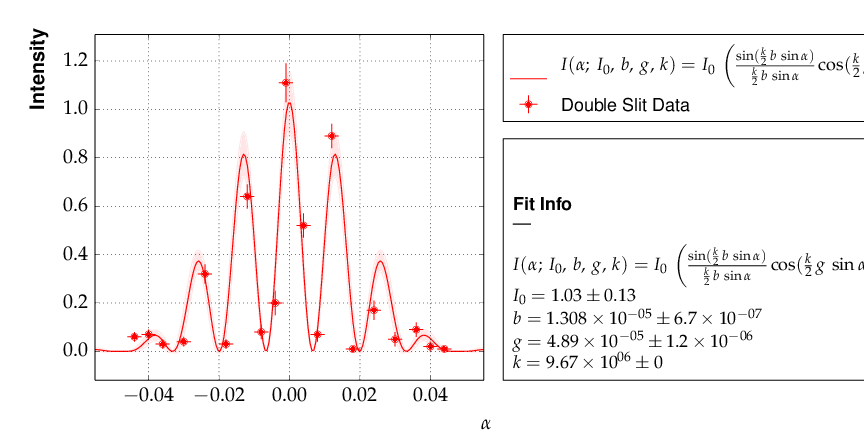
\includegraphics{kafe_example7.png}}
\caption{\emph{Example 7 - fit of the intensity distribution of light behind a double slit with fixed or constrained wave length.}}\end{figure}


\section{Example 8 - fit of a Breit-Wigner Resonance to data with correlated errors}
\label{index:example-8-fit-of-a-breit-wigner-resonance-to-data-with-correlated-errors}
This example illustrates how to define the data and the fit function
in a single file - provided by the helper function \code{buildFit\_fromFile}
in module \code{file\_tools}. Parsing of the input file is done by the
function \code{parse\_general\_inputfile}, which had already been introduced
in Example 4. The definition of the fit function as python code
including the \emph{kafe} decorators in the input file, however, is new.
Note: because spaces are used to to separate data  fields in the
input file, spaces needed for proper python indentation have to be
replaced by `\textasciitilde{}'. The last key in the file defines the start values
of the parameters and their initial ranges.

The advantage of this approach is the location of all data
and the fit model in one place, which is strictly separated
from the python code. The python code below is thus very general
and can handle a large large variety of problems without
modification (except for the file name, which could easily be
passed on the command line):

\begin{Verbatim}[commandchars=\\\{\}]
\PYG{k+kn}{from} \PYG{n+nn}{kafe} \PYG{k+kn}{import} \PYG{o}{*}
\PYG{k+kn}{from} \PYG{n+nn}{kafe.file\PYGZus{}tools} \PYG{k+kn}{import} \PYG{n}{buildFit\PYGZus{}fromFile}
\PYG{c}{\PYGZsh{} \PYGZhy{}\PYGZhy{}\PYGZhy{}\PYGZhy{}\PYGZhy{}\PYGZhy{}\PYGZhy{}\PYGZhy{}\PYGZhy{}\PYGZhy{}\PYGZhy{}\PYGZhy{}\PYGZhy{}\PYGZhy{}\PYGZhy{}\PYGZhy{}\PYGZhy{}\PYGZhy{}\PYGZhy{}\PYGZhy{}\PYGZhy{}\PYGZhy{}\PYGZhy{}\PYGZhy{}\PYGZhy{}\PYGZhy{}\PYGZhy{}\PYGZhy{}\PYGZhy{}\PYGZhy{}\PYGZhy{}\PYGZhy{}\PYGZhy{}\PYGZhy{}\PYGZhy{}\PYGZhy{}\PYGZhy{}\PYGZhy{}\PYGZhy{}\PYGZhy{}\PYGZhy{}\PYGZhy{}\PYGZhy{}\PYGZhy{}\PYGZhy{}\PYGZhy{}\PYGZhy{}\PYGZhy{}\PYGZhy{}\PYGZhy{}\PYGZhy{}\PYGZhy{}\PYGZhy{}\PYGZhy{}\PYGZhy{}\PYGZhy{}\PYGZhy{}}
\PYG{n}{fname} \PYG{o}{=} \PYG{l+s}{\PYGZsq{}}\PYG{l+s}{LEP\PYGZhy{}Data.dat}\PYG{l+s}{\PYGZsq{}}
\PYG{c}{\PYGZsh{} initialize fit object from file}
\PYG{n}{BWfit} \PYG{o}{=} \PYG{n}{buildFit\PYGZus{}fromFile}\PYG{p}{(}\PYG{n}{fname}\PYG{p}{)}
\PYG{n}{BWfit}\PYG{o}{.}\PYG{n}{do\PYGZus{}fit}\PYG{p}{(}\PYG{p}{)}
\PYG{c}{\PYGZsh{}}
\PYG{n}{BWplot} \PYG{o}{=} \PYG{n}{Plot}\PYG{p}{(}\PYG{n}{BWfit}\PYG{p}{)}
\PYG{n}{BWplot}\PYG{o}{.}\PYG{n}{plot\PYGZus{}all}\PYG{p}{(}\PYG{p}{)}
\PYG{n}{BWplot}\PYG{o}{.}\PYG{n}{save}\PYG{p}{(}\PYG{l+s}{\PYGZdq{}}\PYG{l+s}{plot.pdf}\PYG{l+s}{\PYGZdq{}}\PYG{p}{)}
\PYG{n}{BWplot}\PYG{o}{.}\PYG{n}{show}\PYG{p}{(}\PYG{p}{)}
\end{Verbatim}

The magic happens in the input file, which now has to provide
all the information needed to perform the fit:

\begin{Verbatim}[commandchars=\\\{\}]
\# Fit of a Breit-Wigner function to
\#      measurements of hadronic Z cross sections at LEP
\# - - - - - - - - - - - - - - - - - - - - - - - - - - - - - - - -
\#  Meta-data for plotting
*TITLE  LEP Hadronic Cross Section (\$\PYGZbs{}sigma\textasciicircum{}0\_\PYGZbs{}mathrm\PYGZob{}had\PYGZcb{}\$)
*xLabel \$E\_CM\$
*xUnit  \$\PYGZbs{}mathrm\PYGZob{}GeV\PYGZcb{}\$
*yLabel \$\PYGZbs{}sigma\textasciicircum{}0\_\PYGZob{}\PYGZbs{}mathrm\PYGZob{}had\PYGZcb{}\PYGZcb{}\$
*yUnit  \$\PYGZbs{}mathrm\PYGZob{}nb\PYGZcb{}\$

\#----------------------------------------------------------------------
\# DATA: average of hadronic cross sections measured by
\#  ALEPH, DELPHI, L3 and OPAL around 7 energy points at the Z resonance
\#----------------------------------------------------------------------

\# CMenergy E err
*xData
 88.387  0.005
 89.437  0.0015
 90.223  0.005
 91.238  0.003
 92.059  0.005
 93.004  0.0015
 93.916  0.005
\# Centre-of-mass energy has a common uncertainty
*xAbsCor 0.0017

\# sig\textasciicircum{}0\_h  sig err     \#  rad.cor  sig\_h measured
*yData
 6.803   0.036      \#  1.7915    5.0114
 13.965  0.013      \#  4.0213    9.9442
 26.113  0.075      \#  7.867    18.2460
 41.364  0.010      \#  10.8617  30.5022
 27.535  0.088      \#  3.9164   23.6187
 13.362  0.015      \# -0.6933   14.0552
  7.302  0.045      \# -1.8181    9.1196
\# cross-sections have a common relative error
*yRelCor 0.0007

*FITLABEL Breit-Wigner-Fit \PYGZob{}\PYGZbs{}large\PYGZob{}( with s-dependent width )\PYGZcb{}\PYGZcb{}
*FitFunction
\# Breit-Wigner with s-dependent width
@ASCII(expression='s0*E\textasciicircum{}2*G\textasciicircum{}2/[(E\textasciicircum{}2-M\textasciicircum{}2)\textasciicircum{}2+(E\textasciicircum{}4*G\textasciicircum{}2/M\textasciicircum{}2)]')
@LaTeX(name='f', parameter\_names=('\PYGZbs{}\PYGZbs{}sigma\textasciicircum{}0', 'M\_Z','\PYGZbs{}\PYGZbs{}Gamma\_Z'),
expression='\PYGZbs{}\PYGZbs{}frac\PYGZob{}\PYGZbs{}\PYGZbs{}sigma\textasciicircum{}0\PYGZbs{}\PYGZbs{}, M\_Z\textasciicircum{}2\PYGZbs{}\PYGZbs{}Gamma\textasciicircum{}2\PYGZcb{}'
               '\PYGZob{}((E\textasciicircum{}2-M\_Z\textasciicircum{}2)\textasciicircum{}2+(E\textasciicircum{}4\PYGZbs{}\PYGZbs{}Gamma\textasciicircum{}2 / M\_Z\textasciicircum{}2))\PYGZcb{}')
@FitFunction
def fitf(E, M=91.2, G=2.5, s0=41.0):
\textasciitilde{}\textasciitilde{}return s0*E*E*G*G/((E*E-M*M)**2+(E**4*G*G/(M*M)))

*InitialParameters    \# set initial values and ranges
91.2 0.1
2.5  0.1
41.  0.5
\end{Verbatim}

Here is the output:
\begin{figure}[htbp]
\centering
\capstart

\scalebox{1.000000}{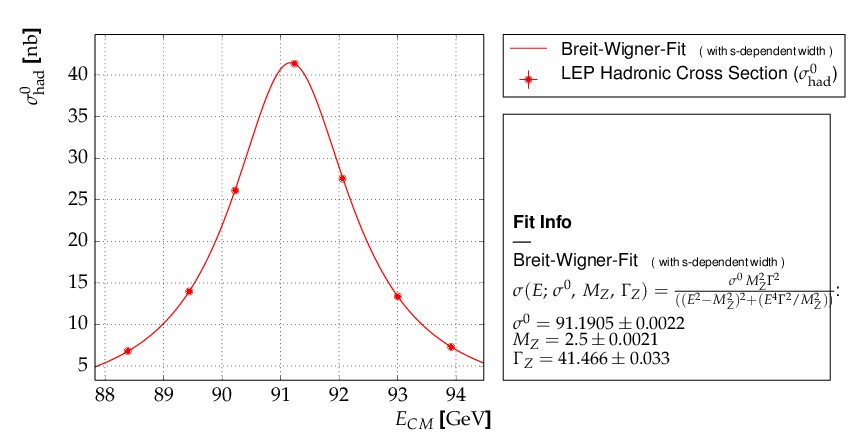
\includegraphics{kafe_BreitWignerFit.png}}
\caption{\emph{Output of example 8 - Fit of a Breit-Wigner function.}}\end{figure}

This example also contains a code snippet demonstrating how to plot
contours with \code{kafe}. A \emph{contour} is a region of the parameter
space containing all parameter values consistent with the fit, within
uncertainty.

Contours are useful because they provide a way to visualize parameter
uncertainties and correlations. \code{kafe} supports plotting
2D $1\sigma$ contours for any pair of parameters by getting the
relevant data from \code{TMinuit} and plotting it using \code{matplotlib}.
Here is a possible way to do it:

\begin{Verbatim}[commandchars=\\\{\}]
\PYG{c}{\PYGZsh{} plot 1\PYGZhy{}sigma contour of first two parameters into a separate figure}
\PYG{n}{x}\PYG{p}{,} \PYG{n}{y} \PYG{o}{=} \PYG{n}{BWfit}\PYG{o}{.}\PYG{n}{minimizer}\PYG{o}{.}\PYG{n}{get\PYGZus{}contour}\PYG{p}{(}\PYG{l+m+mi}{0}\PYG{p}{,} \PYG{l+m+mi}{1}\PYG{p}{,} \PYG{n}{n\PYGZus{}points}\PYG{o}{=}\PYG{l+m+mi}{100}\PYG{p}{)}  \PYG{c}{\PYGZsh{} get contour}
\PYG{n}{cont\PYGZus{}fig} \PYG{o}{=} \PYG{n}{plt}\PYG{o}{.}\PYG{n}{figure}\PYG{p}{(}\PYG{p}{)}  \PYG{c}{\PYGZsh{} create new figure for contour}
\PYG{n}{cont\PYGZus{}ax} \PYG{o}{=} \PYG{n}{cont\PYGZus{}fig}\PYG{o}{.}\PYG{n}{gca}\PYG{p}{(}\PYG{p}{)}  \PYG{c}{\PYGZsh{} get/create axes object for current figure}
\PYG{c}{\PYGZsh{} set axis labels}
\PYG{n}{cont\PYGZus{}ax}\PYG{o}{.}\PYG{n}{set\PYGZus{}xlabel}\PYG{p}{(}\PYG{l+s}{\PYGZsq{}}\PYG{l+s}{\PYGZdl{}}\PYG{l+s+si}{\PYGZpc{}s}\PYG{l+s}{\PYGZdl{}}\PYG{l+s}{\PYGZsq{}} \PYG{o}{\PYGZpc{}} \PYG{p}{(}\PYG{n}{BWfit}\PYG{o}{.}\PYG{n}{latex\PYGZus{}parameter\PYGZus{}names}\PYG{p}{[}\PYG{l+m+mi}{0}\PYG{p}{]}\PYG{p}{,}\PYG{p}{)}\PYG{p}{)}
\PYG{n}{cont\PYGZus{}ax}\PYG{o}{.}\PYG{n}{set\PYGZus{}ylabel}\PYG{p}{(}\PYG{l+s}{\PYGZsq{}}\PYG{l+s}{\PYGZdl{}}\PYG{l+s+si}{\PYGZpc{}s}\PYG{l+s}{\PYGZdl{}}\PYG{l+s}{\PYGZsq{}} \PYG{o}{\PYGZpc{}} \PYG{p}{(}\PYG{n}{BWfit}\PYG{o}{.}\PYG{n}{latex\PYGZus{}parameter\PYGZus{}names}\PYG{p}{[}\PYG{l+m+mi}{1}\PYG{p}{]}\PYG{p}{,}\PYG{p}{)}\PYG{p}{)}
\PYG{c}{\PYGZsh{} plot the actual contour}
\PYG{n}{cont\PYGZus{}ax}\PYG{o}{.}\PYG{n}{fill}\PYG{p}{(}\PYG{n}{x}\PYG{p}{,} \PYG{n}{y}\PYG{p}{,} \PYG{n}{alpha}\PYG{o}{=}\PYG{l+m+mf}{0.25}\PYG{p}{,} \PYG{n}{color}\PYG{o}{=}\PYG{l+s}{\PYGZsq{}}\PYG{l+s}{red}\PYG{l+s}{\PYGZsq{}}\PYG{p}{)}
\PYG{c}{\PYGZsh{} save to file}
\PYG{n}{cont\PYGZus{}fig}\PYG{o}{.}\PYG{n}{savefig}\PYG{p}{(}\PYG{l+s}{\PYGZdq{}}\PYG{l+s}{kafe\PYGZus{}BreitWignerFit\PYGZus{}contour12.pdf}\PYG{l+s}{\PYGZdq{}}\PYG{p}{)}
\end{Verbatim}
\begin{figure}[htbp]
\centering
\capstart

\scalebox{1.000000}{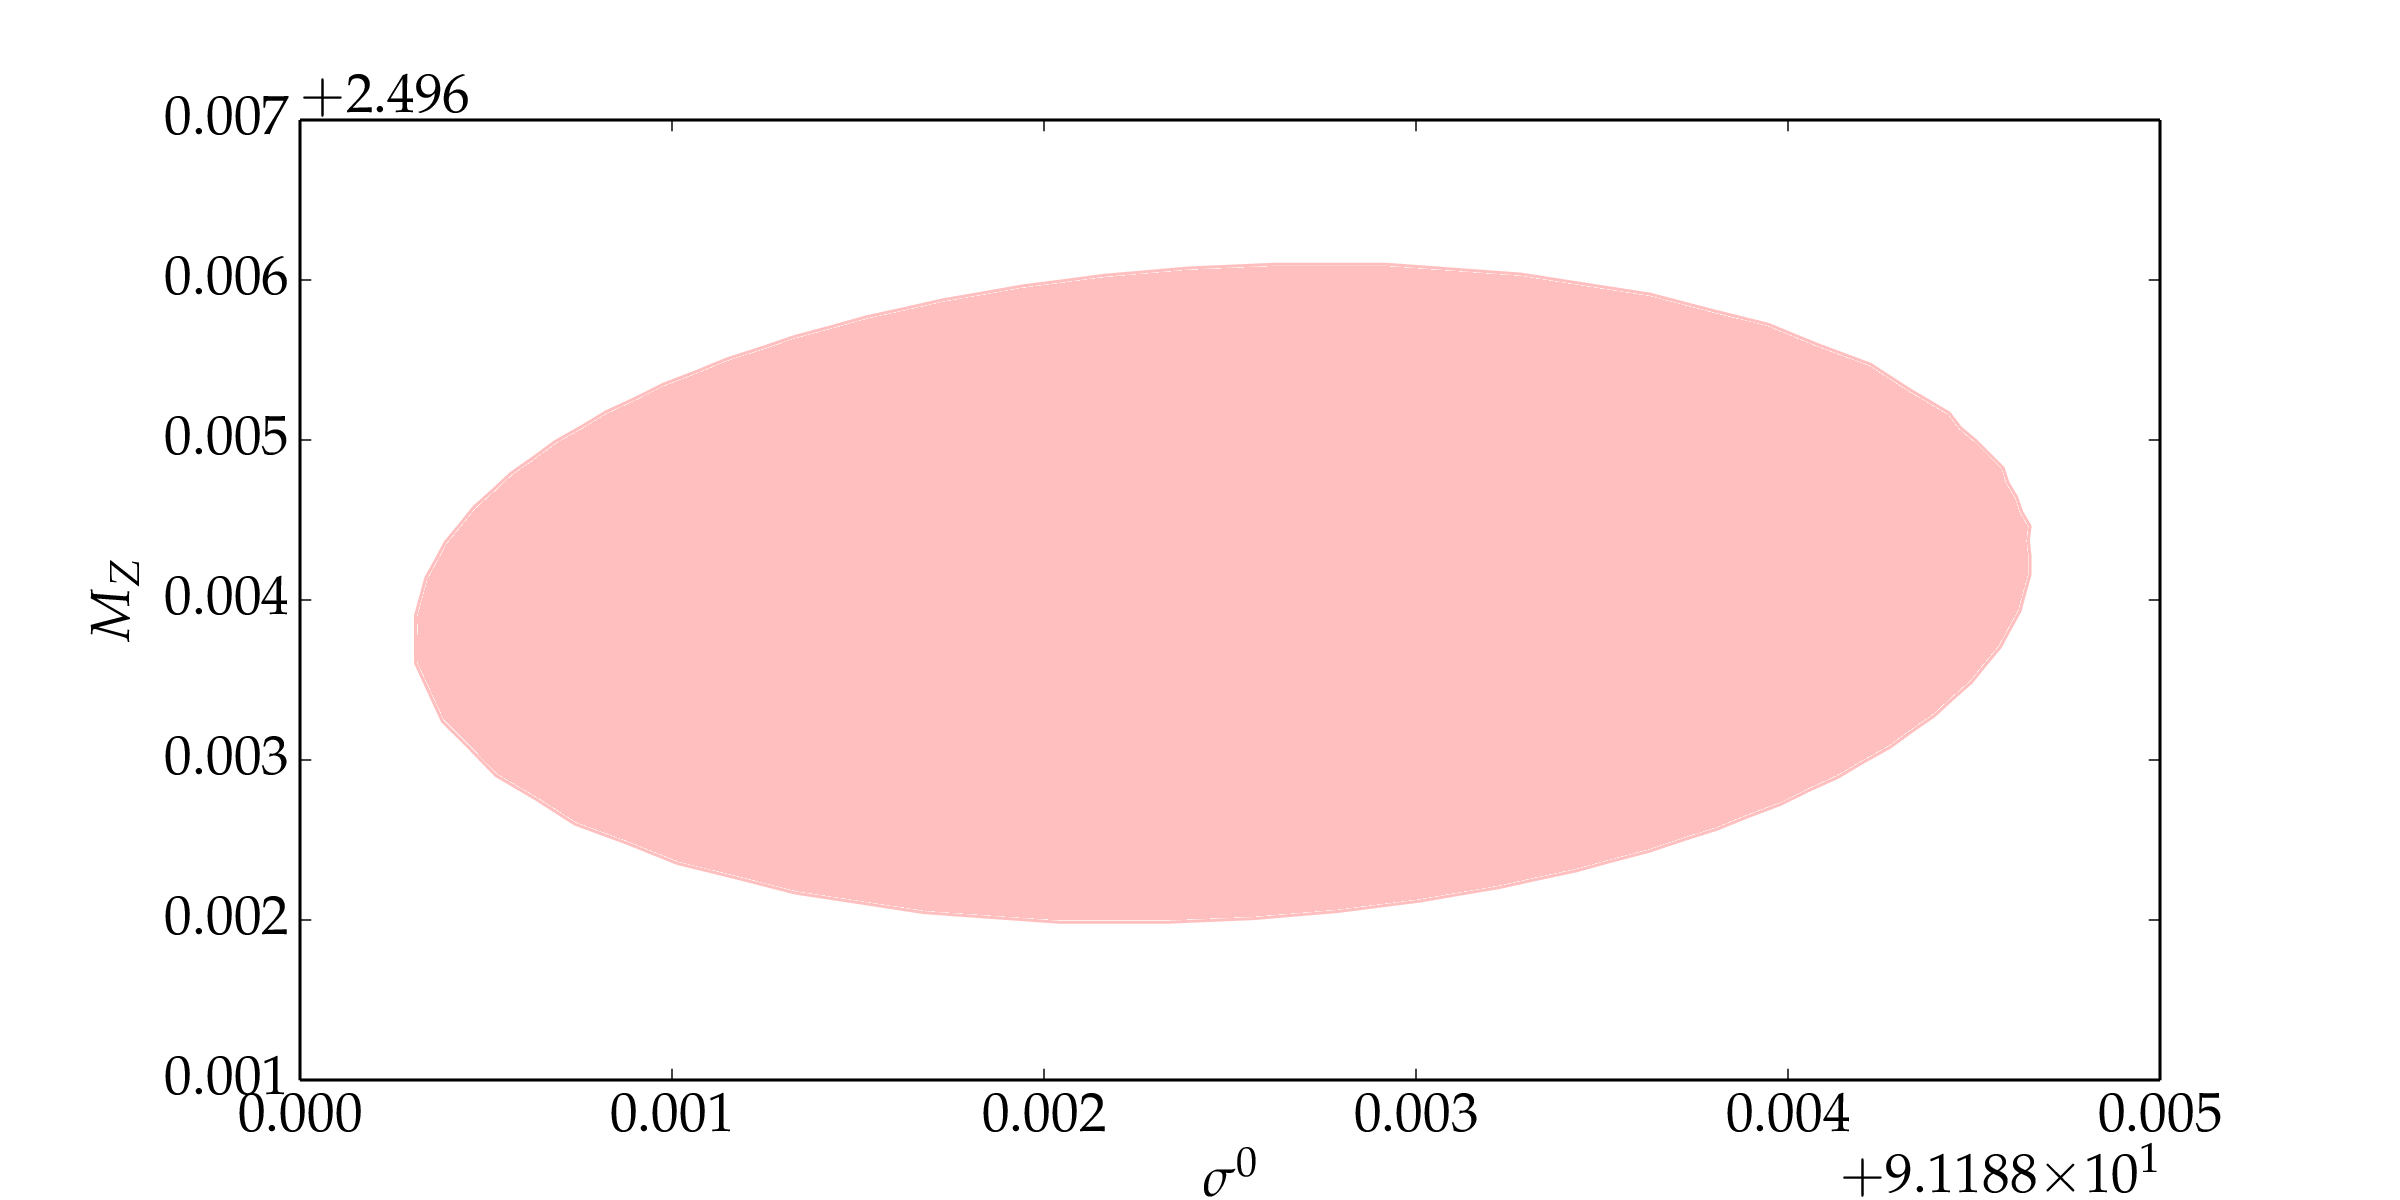
\includegraphics{kafe_BreitWignerFit_contour12.png}}
\caption{\emph{Contour generated in example 8 - Fit of a Breit-Wigner function.}}\end{figure}


\section{Example 9 - fit of a function to histogram data}
\label{index:example-9-fit-of-a-function-to-histogram-data}
This example brings us to the limit of what is currently
possible with \emph{kafe}. Here, the data represent the
centre of a histogram bins ad the number of entries, $n_i$,
in each bin. The (statistical) error is typically estimated
as the square root of the (observed) number of entries in each bin.
For large numbers of entries, this is not a problem,
but for small numbers, especially for bins with 0 entries,
the correlation between the observed number of entries and
the error derived from it leads to a bias when fitting
functions to the histogram data. In particular, bins with
zero entries cannot be handled in the \(\chi\)²-function, and are
typically omitted to cure the problem.  However, a bias
remains, as bins with downward fluctuations of the
observed numbers of events get assigned smaller errors
and hence larger weights in the fitting procedure - leading
to the aforementioned bias.

These problems are avoided by using a likelihood method for
such use cases, where the Poission distribution of the uncertainties
and their dependence on the values of the fit model is properly
taken into accout. However, the \(\chi\)²-method can be saved to some
extend if the fitting procedure is iterated. In a pre-fit, a
first approximation of the model function is determined, where
the error in bins with zero entries is set to one. The model
function determined from the pre-fit is then used to calculate
the expected errors for each bin, and the origial errors are
replaced before performing the final fit. Note that the numbers
of entries in the bins must be sufficiently large to justify
a replacement of the (asymmetric) Poission uncertainties by
the symmetric uncertainties implied by the \(\chi\)²-method.

The code shown below demonstrates
how to get a grip on such more complex procedures with
more fundamental methods of the \emph{Dataset}, \emph{Fit} and
\emph{FitFunction} classes:

\begin{Verbatim}[commandchars=\\\{\}]
\PYG{o}{.}\PYG{o}{.}\PYG{o}{.}
\PYG{c}{\PYGZsh{} Load Dataset from file}
\PYG{n}{hdataset} \PYG{o}{=} \PYG{n}{Dataset}\PYG{p}{(}\PYG{n}{input\PYGZus{}file}\PYG{o}{=}\PYG{l+s}{\PYGZsq{}}\PYG{l+s}{hdataset.dat}\PYG{l+s}{\PYGZsq{}}\PYG{p}{,} \PYG{n}{title}\PYG{o}{=}\PYG{l+s}{\PYGZdq{}}\PYG{l+s}{Data for example 9}\PYG{l+s}{\PYGZdq{}}\PYG{p}{)}

\PYG{c}{\PYGZsh{} error for bins with zero contents is set to 1.}
\PYG{n}{covmat} \PYG{o}{=} \PYG{n}{hdataset}\PYG{o}{.}\PYG{n}{get\PYGZus{}cov\PYGZus{}mat}\PYG{p}{(}\PYG{l+s}{\PYGZsq{}}\PYG{l+s}{y}\PYG{l+s}{\PYGZsq{}}\PYG{p}{)}
\PYG{k}{for} \PYG{n}{i} \PYG{o+ow}{in} \PYG{n+nb}{range}\PYG{p}{(}\PYG{l+m+mi}{0}\PYG{p}{,}\PYG{n+nb}{len}\PYG{p}{(}\PYG{n}{covmat}\PYG{p}{)}\PYG{p}{)}\PYG{p}{:}
    \PYG{k}{if} \PYG{n}{covmat}\PYG{p}{[}\PYG{n}{i}\PYG{p}{,} \PYG{n}{i}\PYG{p}{]}\PYG{o}{==}\PYG{l+m+mf}{0.}\PYG{p}{:}
        \PYG{n}{covmat}\PYG{p}{[}\PYG{n}{i}\PYG{p}{,} \PYG{n}{i}\PYG{p}{]}\PYG{o}{=}\PYG{l+m+mf}{1.}
\PYG{n}{hdataset}\PYG{o}{.}\PYG{n}{set\PYGZus{}cov\PYGZus{}mat}\PYG{p}{(}\PYG{l+s}{\PYGZsq{}}\PYG{l+s}{y}\PYG{l+s}{\PYGZsq{}}\PYG{p}{,} \PYG{n}{covmat}\PYG{p}{)} \PYG{c}{\PYGZsh{} write it back}

\PYG{c}{\PYGZsh{} Create the Fit instance}
\PYG{n}{hfit} \PYG{o}{=} \PYG{n}{Fit}\PYG{p}{(}\PYG{n}{hdataset}\PYG{p}{,} \PYG{n}{gauss}\PYG{p}{,} \PYG{n}{fit\PYGZus{}label}\PYG{o}{=}\PYG{l+s}{\PYGZdq{}}\PYG{l+s}{Fit of a Gaussian to histogram data}\PYG{l+s}{\PYGZdq{}}\PYG{p}{)}
\PYG{c}{\PYGZsh{}}
\PYG{c}{\PYGZsh{} perform an initial fit with temporary errors (minimial output)}
\PYG{n}{hfit}\PYG{o}{.}\PYG{n}{call\PYGZus{}minimizer}\PYG{p}{(}\PYG{n}{final\PYGZus{}fit}\PYG{o}{=}\PYG{n+nb+bp}{False}\PYG{p}{,} \PYG{n}{verbose}\PYG{o}{=}\PYG{n+nb+bp}{False}\PYG{p}{)}
\PYG{c}{\PYGZsh{}}
\PYG{c}{\PYGZsh{}re\PYGZhy{}set errors using model at pre\PYGZhy{}fit parameter values:}
\PYG{c}{\PYGZsh{}        sigma\PYGZus{}i\PYGZca{}2=cov[i,i]=n(x\PYGZus{}i)}
\PYG{n}{fdata}\PYG{o}{=}\PYG{n}{hfit}\PYG{o}{.}\PYG{n}{fit\PYGZus{}function}\PYG{o}{.}\PYG{n}{evaluate}\PYG{p}{(}\PYG{n}{hfit}\PYG{o}{.}\PYG{n}{xdata}\PYG{p}{,} \PYG{n}{hfit}\PYG{o}{.}\PYG{n}{current\PYGZus{}parameter\PYGZus{}values}\PYG{p}{)}
\PYG{n}{np}\PYG{o}{.}\PYG{n}{fill\PYGZus{}diagonal}\PYG{p}{(}\PYG{n}{covmat}\PYG{p}{,} \PYG{n}{fdata}\PYG{p}{)}
\PYG{n}{hfit}\PYG{o}{.}\PYG{n}{current\PYGZus{}cov\PYGZus{}mat} \PYG{o}{=} \PYG{n}{covmat} \PYG{c}{\PYGZsh{} write back new covariance matrix}
\PYG{c}{\PYGZsh{}}
\PYG{c}{\PYGZsh{} now do final fit with full output}
\PYG{n}{hfit}\PYG{o}{.}\PYG{n}{do\PYGZus{}fit}\PYG{p}{(}\PYG{p}{)}
\PYG{c}{\PYGZsh{} and create, draw, save and show plot}
\PYG{o}{.}\PYG{o}{.}\PYG{o}{.}
\end{Verbatim}

Here is the output, which shows that the parameters of the
normal distribution, from which the data were generated, are
well reproduced within the uncertainties by the fit result:
\begin{figure}[htbp]
\centering
\capstart

\scalebox{1.000000}{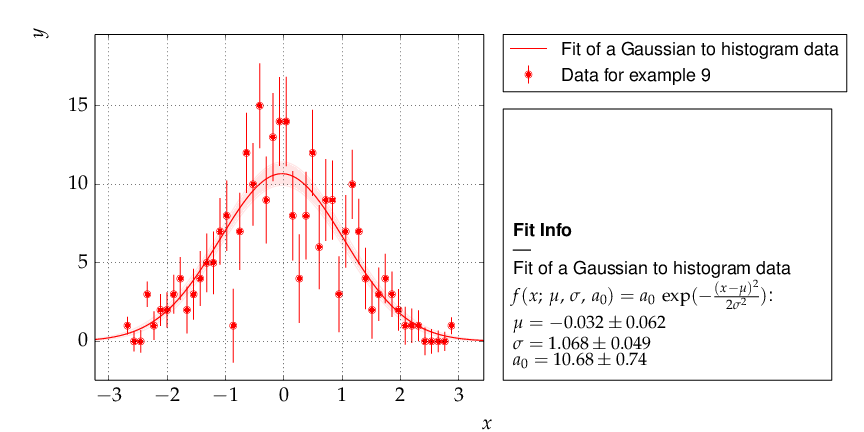
\includegraphics{kafe_example9.png}}
\caption{\emph{Output of example 9 - Fit of a Gaussian distribution to histogram data}}\end{figure}


\chapter{\emph{kafe} Documentation -- module descriptions}
\label{index:kafe-documentation-module-descriptions}
The following documentation of functions and methods
of relevance to the user interface was generated from
the \emph{DocStrings} contained in the python code of the
\emph{kafe} package.
For further information or if in doubt about the exact
functionality, users are invited to consult the source
code.


\section{\texttt{kafe.\_\_init\_\_} Module}
\label{index:module-kafe.__init__}\label{index:kafe-init-module}\index{kafe.\_\_init\_\_ (module)}
\textbf{kafe} \emph{-- a Python package for fitting and plotting for use in physics lab courses.}

This Python package allows fitting of user-defined functions to data. A dataset
is represented by a \emph{Dataset} object which stores measurement data as \emph{NumPy}
arrays. The uncertainties of the data are also stored in the \emph{Dataset} as an
\emph{error matrix}, allowing for both correlated and uncorrelated errors to be
accurately represented.

The constructor of a \emph{Dataset} object accepts several keyword arguments and can
be used to construct a \emph{Dataset} from input data which has been loaded into
\emph{Python} as \emph{NumPy} arrays. Alternatively, a plain-text representations of a
\emph{Dataset} can be read from a file.

Also provided are helper functions which construct a \emph{Dataset} object from a
file containing column data (one measurement per row, column order can be
specified), or from a keyword-driven input format.


\section{\texttt{\_version\_info} Module}
\label{index:module-kafe._version_info}\label{index:version-info-module}\index{kafe.\_version\_info (module)}\phantomsection\label{index:module-__version_info}\index{\_\_version\_info (module)}\index{get\_version() (in module kafe.\_version\_info)}

\begin{fulllineitems}
\phantomsection\label{index:kafe._version_info.get_version}\pysiglinewithargsret{\code{kafe.\_version\_info.}\bfcode{get\_version}}{}{}
kafe version 0.5.2

\end{fulllineitems}



\section{\texttt{dataset} Module}
\label{index:dataset-module}\label{index:module-kafe.dataset}\index{kafe.dataset (module)}\phantomsection\label{index:module-dataset}\index{dataset (module)}\index{Dataset (class in kafe.dataset)}

\begin{fulllineitems}
\phantomsection\label{index:kafe.dataset.Dataset}\pysiglinewithargsret{\strong{class }\code{kafe.dataset.}\bfcode{Dataset}}{\emph{input\_file=None, data=None, cov\_mats=None, title='Untitled Dataset', basename=None, axis\_labels={[}'x', `y'{]}, axis\_units={[}'`, `'{]}}}{}
Bases: \code{object}

The \emph{Dataset} object is a data structure for storing measurement and error
data. In this implementation, the \emph{Dataset} has the compulsory field
\emph{data}, which is used for storing the measurement data, and another field
\emph{cov\_mats}, used for storing the covariance matrix for each axis.

There are two ways a \emph{Dataset} can be constructed. The most
straightforward way is to specify an input file containing a plain-text
representation of the dataset:

\begin{Verbatim}[commandchars=\\\{\}]
\PYG{g+gp}{\PYGZgt{}\PYGZgt{}\PYGZgt{} }\PYG{n}{my\PYGZus{}dataset} \PYG{o}{=} \PYG{n}{Dataset}\PYG{p}{(}\PYG{n}{input\PYGZus{}file}\PYG{o}{=}\PYG{l+s}{\PYGZsq{}}\PYG{l+s}{/path/to/file}\PYG{l+s}{\PYGZsq{}}\PYG{p}{)}
\end{Verbatim}

or

\begin{Verbatim}[commandchars=\\\{\}]
\PYG{g+gp}{\PYGZgt{}\PYGZgt{}\PYGZgt{} }\PYG{n}{my\PYGZus{}dataset} \PYG{o}{=} \PYG{n}{Dataset}\PYG{p}{(}\PYG{n}{input\PYGZus{}file}\PYG{o}{=}\PYG{n}{my\PYGZus{}file\PYGZus{}object}\PYG{p}{)}
\end{Verbatim}

If an \emph{input\_file} argument is provided, the \emph{data} and \emph{cov\_mats}
arguments are ignored. The \emph{Dataset} plain-text representation format
is as follows:

\begin{Verbatim}[commandchars=\\\{\}]
\# x data
x\_1  sigma\_x\_1
x\_2  sigma\_x\_2  cor\_x\_12
...  ...        ...       ...
x\_N  sigma\_x\_N  cor\_x\_1N  ...  cor\_x\_NN

\# y data
y\_1  sigma\_y\_1
y\_2  sigma\_y\_2  cor\_y\_12
...  ...        ...       ...
y\_N  sigma\_y\_N  cor\_y\_1N  ...  cor\_y\_NN
\end{Verbatim}

Here, the \emph{sigma\_...} represents the fully uncorrelated error of the data
point and \emph{cor\_...\_ij} is the correlation coefficient between the \emph{i}-th
and \emph{j}-th data point.

Alternatively, field data can be set by passing iterables as arguments.
Available arguments for this purpose are:

\textbf{data} : tuple/list of tuples/lists/arrays of floats
\begin{quote}

a tuple/list of measurement data. Each element of the tuple/list must
be iterable and be of the same length. The first element of the
\textbf{data} tuple/list is assumed to be the \emph{x} data, and the second to be
the \emph{y} data:

\begin{Verbatim}[commandchars=\\\{\}]
\PYG{g+gp}{\PYGZgt{}\PYGZgt{}\PYGZgt{} }\PYG{n}{my\PYGZus{}dataset} \PYG{o}{=} \PYG{n}{Dataset}\PYG{p}{(}\PYG{n}{data}\PYG{o}{=}\PYG{p}{(}\PYG{p}{[}\PYG{l+m+mf}{0.}\PYG{p}{,} \PYG{l+m+mf}{1.}\PYG{p}{,} \PYG{l+m+mf}{2.}\PYG{p}{]}\PYG{p}{,} \PYG{p}{[}\PYG{l+m+mf}{1.23}\PYG{p}{,} \PYG{l+m+mf}{3.45}\PYG{p}{,} \PYG{l+m+mf}{5.62}\PYG{p}{]}\PYG{p}{)}\PYG{p}{)}
\end{Verbatim}

Alternatively, x-y value pairs can also be passed as \textbf{data}. The
following is equivalent to the above:

\begin{Verbatim}[commandchars=\\\{\}]
\PYG{g+gp}{\PYGZgt{}\PYGZgt{}\PYGZgt{} }\PYG{n}{my\PYGZus{}dataset} \PYG{o}{=} \PYG{n}{Dataset}\PYG{p}{(}\PYG{n}{data}\PYG{o}{=}\PYG{p}{(}\PYG{p}{[}\PYG{l+m+mf}{0.0}\PYG{p}{,} \PYG{l+m+mf}{1.23}\PYG{p}{]}\PYG{p}{,} \PYG{p}{[}\PYG{l+m+mf}{1.0}\PYG{p}{,} \PYG{l+m+mf}{3.45}\PYG{p}{]}\PYG{p}{,} \PYG{p}{[}\PYG{l+m+mf}{2.0}\PYG{p}{,} \PYG{l+m+mf}{5.62}\PYG{p}{]}\PYG{p}{)}\PYG{p}{)}
\end{Verbatim}

In case the \emph{Dataset} contains two data points, the ordering is
ambiguous. In this case, the first ordering (\emph{x} data first, then \emph{y}
data) is assumed.
\end{quote}

\emph{cov\_mats} : tuple/list of \emph{numpy.matrix} (optional)
\begin{quote}

a tuple/list of two-dimensional iterables containing the covariance
matrices for \emph{x} and \emph{y}, in that order. Covariance matrices can be any
sort of two-dimensional NxN iterables, assuming N is the number of data
points.

\begin{Verbatim}[commandchars=\\\{\}]
\PYG{g+gp}{\PYGZgt{}\PYGZgt{}\PYGZgt{} }\PYG{n}{my\PYGZus{}dataset} \PYG{o}{=} \PYG{n}{Dataset}\PYG{p}{(}\PYG{n}{data}\PYG{o}{=}\PYG{p}{(}\PYG{p}{[}\PYG{l+m+mf}{0.}\PYG{p}{,} \PYG{l+m+mf}{1.}\PYG{p}{,} \PYG{l+m+mf}{2.}\PYG{p}{]}\PYG{p}{,} \PYG{p}{[}\PYG{l+m+mf}{1.23}\PYG{p}{,} \PYG{l+m+mf}{3.45}\PYG{p}{,} \PYG{l+m+mf}{5.62}\PYG{p}{]}\PYG{p}{)}\PYG{p}{,} \PYG{n}{cov\PYGZus{}mats}\PYG{o}{=}\PYG{p}{(}\PYG{n}{my\PYGZus{}cov\PYGZus{}mat\PYGZus{}x}\PYG{p}{,} \PYG{n}{my\PYGZus{}cov\PYGZus{}mat\PYGZus{}y}\PYG{p}{)}\PYG{p}{)}
\end{Verbatim}

This keyword argument can be omitted, in which case covariance matrices
of zero are assumed. To specify a covariance matrix for a single axis,
replace the other with \code{None}.

\begin{Verbatim}[commandchars=\\\{\}]
\PYG{g+gp}{\PYGZgt{}\PYGZgt{}\PYGZgt{} }\PYG{n}{my\PYGZus{}dataset} \PYG{o}{=} \PYG{n}{Dataset}\PYG{p}{(}\PYG{n}{data}\PYG{o}{=}\PYG{p}{(}\PYG{p}{[}\PYG{l+m+mf}{0.}\PYG{p}{,} \PYG{l+m+mf}{1.}\PYG{p}{,} \PYG{l+m+mf}{2.}\PYG{p}{]}\PYG{p}{,} \PYG{p}{[}\PYG{l+m+mf}{1.23}\PYG{p}{,} \PYG{l+m+mf}{3.45}\PYG{p}{,} \PYG{l+m+mf}{5.62}\PYG{p}{]}\PYG{p}{)}\PYG{p}{,} \PYG{n}{cov\PYGZus{}mats}\PYG{o}{=}\PYG{p}{(}\PYG{n+nb+bp}{None}\PYG{p}{,} \PYG{n}{my\PYGZus{}cov\PYGZus{}mat\PYGZus{}y}\PYG{p}{)}\PYG{p}{)}
\end{Verbatim}
\end{quote}

\emph{title} : string (optional)
\begin{quote}

the name of the \emph{Dataset}. If omitted, the \emph{Dataset} will be given the
generic name `Untitled Dataset'.
\end{quote}

\emph{axis\_labels} : list of strings (optional)
\begin{quote}

labels for the \emph{x} and \emph{y} axes. If omitted, these will be set to
\code{'x'} and \code{'y'}, respectively.
\end{quote}

\emph{axis\_units} : list of strings (optional)
\begin{quote}

units for the \emph{x} and \emph{y} axes. If omitted, these will be assumed to be
dimensionless, i.e. the unit will be an empty string.
\end{quote}
\index{cov\_mat\_is\_regular() (kafe.dataset.Dataset method)}

\begin{fulllineitems}
\phantomsection\label{index:kafe.dataset.Dataset.cov_mat_is_regular}\pysiglinewithargsret{\bfcode{cov\_mat\_is\_regular}}{\emph{axis}}{}
Returns \emph{True} if the covariance matrix for an axis is regular and
\code{False} if it is singular.
\begin{description}
\item[{\textbf{axis}}] \leavevmode{[}\code{'x'} or \code{'y'}{]}
Axis for which to check for regularity of the covariance matrix.

\end{description}

\end{fulllineitems}

\index{cov\_mats (kafe.dataset.Dataset attribute)}

\begin{fulllineitems}
\phantomsection\label{index:kafe.dataset.Dataset.cov_mats}\pysigline{\bfcode{cov\_mats}\strong{ = None}}
list of covariance matrices

\end{fulllineitems}

\index{get\_axis() (kafe.dataset.Dataset method)}

\begin{fulllineitems}
\phantomsection\label{index:kafe.dataset.Dataset.get_axis}\pysiglinewithargsret{\bfcode{get\_axis}}{\emph{axis\_alias}}{}
Get axis id from an alias.
\begin{description}
\item[{\textbf{axis\_alias}}] \leavevmode{[}string or int{]}
Alias of the axis whose id should be returned. This is for example
either \code{'0'} or \code{'x'} for the \emph{x}-axis (id 0).

\end{description}

\end{fulllineitems}

\index{get\_cov\_mat() (kafe.dataset.Dataset method)}

\begin{fulllineitems}
\phantomsection\label{index:kafe.dataset.Dataset.get_cov_mat}\pysiglinewithargsret{\bfcode{get\_cov\_mat}}{\emph{axis}, \emph{fallback\_on\_singular=None}}{}
Get the error matrix for an axis.
\begin{description}
\item[{\textbf{axis}}] \leavevmode{[}\code{'x'} or \code{'y'}{]}
Axis for which to load the error matrix.

\item[{\emph{fallback\_on\_singular}}] \leavevmode{[}\emph{numpy.matrix} or string (optional){]}
What to return if the matrix is singular. If this is \code{None}
(default), the matrix is returned anyway. If this is a
\emph{numpy.matrix} object or similar, that is returned istead.
Alternatively, the shortcuts \code{'identity'} or \code{1} and \code{'zero'}
or \code{0} can be used to return the identity and zero matrix
respectively.

\end{description}

\end{fulllineitems}

\index{get\_data() (kafe.dataset.Dataset method)}

\begin{fulllineitems}
\phantomsection\label{index:kafe.dataset.Dataset.get_data}\pysiglinewithargsret{\bfcode{get\_data}}{\emph{axis}}{}
Get the measurement data for an axis.
\begin{description}
\item[{\textbf{axis}}] \leavevmode{[}string{]}
Axis for which to get the measurement data. Can be \code{'x'} or
\code{'y'}.

\end{description}

\end{fulllineitems}

\index{get\_data\_span() (kafe.dataset.Dataset method)}

\begin{fulllineitems}
\phantomsection\label{index:kafe.dataset.Dataset.get_data_span}\pysiglinewithargsret{\bfcode{get\_data\_span}}{\emph{axis}, \emph{include\_error\_bars=False}}{}
Get the data span for an axis. The data span is a tuple (\emph{min}, \emph{max})
containing the smallest and highest coordinates for an axis.
\begin{description}
\item[{\textbf{axis}}] \leavevmode{[}\code{'x'} or \code{'y'}{]}
Axis for which to get the data span.

\item[{\emph{include\_error\_bars}}] \leavevmode{[}boolean (optional){]}
\code{True} if the returned span should be enlarged to
contain the error bars of the smallest and largest datapoints
(default: \code{False})

\end{description}

\end{fulllineitems}

\index{get\_formatted() (kafe.dataset.Dataset method)}

\begin{fulllineitems}
\phantomsection\label{index:kafe.dataset.Dataset.get_formatted}\pysiglinewithargsret{\bfcode{get\_formatted}}{\emph{format\_string='.06e'}, \emph{delimiter='t'}}{}
Returns the dataset in a plain-text format which is human-readable and
can later be used as an input file for the creation of a new \emph{Dataset}.
\phantomsection\label{index:get-formatted}
The format is as follows:

\begin{Verbatim}[commandchars=\\\{\}]
\# x data
x\_1  sigma\_x\_1
x\_2  sigma\_x\_2  cor\_x\_12
...  ...        ...       ...
x\_N  sigma\_x\_N  cor\_x\_1N  ...  cor\_x\_NN

\# y data
y\_1  sigma\_y\_1
y\_2  sigma\_y\_2  cor\_y\_12
...  ...        ...       ...
y\_N  sigma\_y\_N  cor\_y\_1N  ...  cor\_y\_NN
\end{Verbatim}

Here, the \code{x\_i} and \code{y\_i} represent the measurement data, the
\code{sigma\_?\_i} are the statistical uncertainties of each data point, and
the \code{cor\_?\_ij} are the correlation coefficients between the \emph{i}-th
and \emph{j}-th data point.

If the \code{x} or \code{y} errors are not correlated, then the entire
correlation coefficient matrix can be omitted. If there are no
statistical uncertainties for an axis, the second column can also be
omitted. A blank line is required at the end of each data block!
\begin{description}
\item[{\emph{format\_string}}] \leavevmode{[}string (optional){]}
A format string with which each entry will be rendered. Default is
\code{'.06e'}, which means the numbers are represented in scientific
notation with six significant digits.

\item[{\emph{delimiter}}] \leavevmode{[}string (optional){]}
A delimiter used to separate columns in the output.

\end{description}

\end{fulllineitems}

\index{get\_size() (kafe.dataset.Dataset method)}

\begin{fulllineitems}
\phantomsection\label{index:kafe.dataset.Dataset.get_size}\pysiglinewithargsret{\bfcode{get\_size}}{}{}
Get the size of the \emph{Dataset}. This is equivalent to the length of the
\emph{x}-axis data.

\end{fulllineitems}

\index{has\_correlations() (kafe.dataset.Dataset method)}

\begin{fulllineitems}
\phantomsection\label{index:kafe.dataset.Dataset.has_correlations}\pysiglinewithargsret{\bfcode{has\_correlations}}{\emph{axis}}{}
Returns \emph{True} if the specified axis has correlation data, \code{False} if
not.
\begin{description}
\item[{\textbf{axis}}] \leavevmode{[}\code{'x'} or \code{'y'}{]}
Axis for which to check for correlations.

\end{description}

\end{fulllineitems}

\index{has\_errors() (kafe.dataset.Dataset method)}

\begin{fulllineitems}
\phantomsection\label{index:kafe.dataset.Dataset.has_errors}\pysiglinewithargsret{\bfcode{has\_errors}}{\emph{axis}}{}
Returns \emph{True} if the specified axis has statistical error data.
\begin{description}
\item[{\textbf{axis}}] \leavevmode{[}\code{'x'} or \code{'y'}{]}
Axis for which to check for error data.

\end{description}

\end{fulllineitems}

\index{n\_axes (kafe.dataset.Dataset attribute)}

\begin{fulllineitems}
\phantomsection\label{index:kafe.dataset.Dataset.n_axes}\pysigline{\bfcode{n\_axes}\strong{ = None}}
dimensionality of the \emph{Dataset}. Currently, only 2D \emph{Datasets} are
supported

\end{fulllineitems}

\index{n\_datapoints (kafe.dataset.Dataset attribute)}

\begin{fulllineitems}
\phantomsection\label{index:kafe.dataset.Dataset.n_datapoints}\pysigline{\bfcode{n\_datapoints}\strong{ = None}}
number of data points in the \emph{Dataset}

\end{fulllineitems}

\index{read\_from\_file() (kafe.dataset.Dataset method)}

\begin{fulllineitems}
\phantomsection\label{index:kafe.dataset.Dataset.read_from_file}\pysiglinewithargsret{\bfcode{read\_from\_file}}{\emph{input\_file}}{}
Reads the \emph{Dataset} object from a file.
\begin{description}
\item[{returns}] \leavevmode{[}boolean{]}
\code{True} if the read succeeded, \code{False} if not.

\end{description}

\end{fulllineitems}

\index{set\_cov\_mat() (kafe.dataset.Dataset method)}

\begin{fulllineitems}
\phantomsection\label{index:kafe.dataset.Dataset.set_cov_mat}\pysiglinewithargsret{\bfcode{set\_cov\_mat}}{\emph{axis}, \emph{mat}}{}
Set the error matrix for an axis.
\begin{description}
\item[{\textbf{axis}}] \leavevmode{[}\code{'x'} or \code{'y'}{]}
Axis for which to load the error matrix.

\item[{\textbf{mat}}] \leavevmode{[}\emph{numpy.matrix} or \code{None}{]}
Error matrix for the axis. Passing \code{None} unsets the error
matrix.

\end{description}

\end{fulllineitems}

\index{set\_data() (kafe.dataset.Dataset method)}

\begin{fulllineitems}
\phantomsection\label{index:kafe.dataset.Dataset.set_data}\pysiglinewithargsret{\bfcode{set\_data}}{\emph{axis}, \emph{data}}{}
Set the measurement data for an axis.
\begin{description}
\item[{\textbf{axis}}] \leavevmode{[}\code{'x'} or \code{'y'}{]}
Axis for which to set the measurement data.

\item[{\textbf{data}}] \leavevmode{[}iterable{]}
Measurement data for axis.

\end{description}

\end{fulllineitems}

\index{write\_formatted() (kafe.dataset.Dataset method)}

\begin{fulllineitems}
\phantomsection\label{index:kafe.dataset.Dataset.write_formatted}\pysiglinewithargsret{\bfcode{write\_formatted}}{\emph{file\_path}, \emph{format\_string='.06e'}, \emph{delimiter='t'}}{}
Writes the dataset to a plain-text file. For details on the format, see
{\hyperref[index:get-formatted]{get\_formatted}}.
\begin{description}
\item[{\textbf{file\_path}}] \leavevmode{[}string{]}
Path of the file object to write. \textbf{WARNING}: \emph{overwrites existing
files}!

\item[{\emph{format\_string}}] \leavevmode{[}string (optional){]}
A format string with which each entry will be rendered. Default is
\code{'.06e'}, which means the numbers are represented in scientific
notation with six significant digits.

\item[{\emph{delimiter}}] \leavevmode{[}string (optional){]}
A delimiter used to separate columns in the output.

\end{description}

\end{fulllineitems}


\end{fulllineitems}

\index{build\_dataset() (in module kafe.dataset)}

\begin{fulllineitems}
\phantomsection\label{index:kafe.dataset.build_dataset}\pysiglinewithargsret{\code{kafe.dataset.}\bfcode{build\_dataset}}{\emph{xdata}, \emph{ydata}, \emph{cov\_mats=None}, \emph{xabserr=0.0}, \emph{xrelerr=0.0}, \emph{xabscor=0.0}, \emph{xrelcor=0.0}, \emph{yabserr=0.0}, \emph{yrelerr=0.0}, \emph{yabscor=0.0}, \emph{yrelcor=0.0}, \emph{title=None}, \emph{basename=None}, \emph{axis\_labels=None}, \emph{axis\_units=None}}{}
This helper function creates a \emph{Dataset} from a series of keyword
arguments.

Valid keyword arguments are:
\begin{description}
\item[{\textbf{xdata} and \textbf{ydata}}] \leavevmode{[}list/tuple/\emph{np.array} of floats{]}
These keyword arguments are mandatory and should be iterables
containing the measurement data.

\item[{\emph{cov\_mats}}] \leavevmode{[}\code{None} or 2-tuple (optional){]}
This argument defaults to \code{None}, which means no covariance matrices
are used. If covariance matrices are needed, a tuple with two entries
(the first for \emph{x} covariance matrices, the second for \emph{y}) must be
passed.

Each element of this tuple may be either \code{None} or a NumPy matrix
object containing a covariance matrix for the respective axis.

\item[{\emph{error specification keywords}}] \leavevmode{[}iterable or numeric (see below){]}
In addition to covariance matrices, errors can be specified for each
axis (\emph{x} or \emph{y}) according to a simplified error model.

In this respect, a valid keyword is composed of an axis, an error
relativity specification (\emph{abs} or \emph{rel}) and error correlation type
(\emph{err} or \emph{cor}). The errors are then set as follows:
\begin{enumerate}
\item {} \begin{description}
\item[{For totally uncorrelated errors (\emph{err}):}] \leavevmode\begin{itemize}
\item {} 
if keyword argument is iterable, the error list is set to that

\item {} 
if keyword argument is a number, an error list with identical entries is generated

\end{itemize}

\end{description}

\item {} \begin{description}
\item[{For fully correlated errors (\emph{cor}):}] \leavevmode\begin{itemize}
\item {} 
keyword argument \emph{must} be a single number. The global correlated error for the axis is then set to that.

\end{itemize}

\end{description}

\end{enumerate}

So, for example:

\begin{Verbatim}[commandchars=\\\{\}]
\PYG{g+gp}{\PYGZgt{}\PYGZgt{}\PYGZgt{} }\PYG{n}{myDataset} \PYG{o}{=} \PYG{n}{build\PYGZus{}dataset}\PYG{p}{(}\PYG{o}{.}\PYG{o}{.}\PYG{o}{.}\PYG{p}{,} \PYG{n}{yabserr}\PYG{o}{=}\PYG{l+m+mf}{0.3}\PYG{p}{,} \PYG{n}{yrelcor}\PYG{o}{=}\PYG{l+m+mf}{0.1}\PYG{p}{)}
\end{Verbatim}

creates a Dataset with an uncorrelated error of 0.3 for each \emph{y}
coordinate and a fully correlated (systematic) error of \emph{y} of 0.1.

\item[{\emph{title}}] \leavevmode{[}string (optional){]}
The title of the \emph{Dataset}.

\item[{\emph{basename}}] \leavevmode{[}string or \code{None} (optional){]}
A basename for the \emph{Dataset}. All output files related to this dataset
will use this as a basename. If this is \code{None} (default), the
basename will be inferred from the filename.

\item[{\emph{axis\_labels}}] \leavevmode{[}2-tuple of strings (optional){]}
a 2-tuple containing the axis labels for the \emph{Dataset}. This is
relevant when plotting \emph{Fits} of the \emph{Dataset}, but is ignored when
plotting more than one \emph{Fit} in the same \emph{Plot}.

\item[{\emph{axis\_units}}] \leavevmode{[}2-tuple of strings (optional){]}
a 2-tuple containing the axis units for the \emph{Dataset}. This is
relevant when plotting \emph{Fits} of the \emph{Dataset}, but is ignored when
plotting more than one \emph{Fit} in the same \emph{Plot}.

\end{description}

\end{fulllineitems}



\section{\texttt{file\_tools} Module}
\label{index:file-tools-module}\label{index:module-kafe.file_tools}\index{kafe.file\_tools (module)}\phantomsection\label{index:module-file_tools}\index{file\_tools (module)}\index{buildDataset\_fromFile() (in module kafe.file\_tools)}

\begin{fulllineitems}
\phantomsection\label{index:kafe.file_tools.buildDataset_fromFile}\pysiglinewithargsret{\code{kafe.file\_tools.}\bfcode{buildDataset\_fromFile}}{\emph{file\_to\_parse}}{}
build a kafe \code{Dataset} object from input file with key words
and file format defined in \code{parse\_general\_inputfile}
\begin{description}
\item[{\textbf{file\_to\_parse}}] \leavevmode{[}file-like object or string containing a file path{]}
The file to parse.

\item[{\textbf{returns}}] \leavevmode{[}an instance of the \code{Dataset} class,{]}
constructed with the help of the method \code{Dataset.build\_dataset()}

\end{description}

\end{fulllineitems}

\index{buildFit\_fromFile() (in module kafe.file\_tools)}

\begin{fulllineitems}
\phantomsection\label{index:kafe.file_tools.buildFit_fromFile}\pysiglinewithargsret{\code{kafe.file\_tools.}\bfcode{buildFit\_fromFile}}{\emph{file\_to\_parse}}{}
build a kafe \code{Fit} object from input file with keywords
and file format defined in \code{parse\_general\_input\_file()}
\begin{description}
\item[{\textbf{file\_to\_parse}:  file-like object or string containing a file path}] \leavevmode
The file to parse.

\item[{\textbf{returns}}] \leavevmode{[}an instance of the \code{Fit} class,{]}
constructed with the help of the methods
\code{Dataset.build\_dataset()} and
\code{Fit.build\_fit()}

\end{description}

\end{fulllineitems}

\index{parse\_column\_data() (in module kafe.file\_tools)}

\begin{fulllineitems}
\phantomsection\label{index:kafe.file_tools.parse_column_data}\pysiglinewithargsret{\code{kafe.file\_tools.}\bfcode{parse\_column\_data}}{\emph{file\_to\_parse, field\_order='x,y', delimiter=' `, cov\_mat\_files=None, title='Untitled Dataset', basename=None, axis\_labels={[}'x', `y'{]}, axis\_units={[}'`, `'{]}}}{}
Parses a file which contains measurement data in a one-measurement-per-row
format. The field (column) order can be specified. It defaults to
\code{"x,y"}.
Valid field names are \emph{x}, \emph{y}, \emph{xabserr}, \emph{yabserr}, \emph{xrelerr},
\emph{yrelerr}. Another valid field name is \emph{ignore} which can be used to skip
a field.

A certain type of field can appear several times. If this is the case, all
specified errors are added in quadrature:
\begin{gather}
\begin{split}\sigma_{\text{tot}} = \sqrt{{\sigma_1}^2+{\sigma_2}^2+\dots}\end{split}\notag
\end{gather}
Every valid measurement data file \emph{must} have an \emph{x} and a \emph{y} field.

For more complex error models, errors and correlations may be specified as
covariance matrices. If this is desired, then any number of covariance
matrices (stored in separate files) may be specified for an axis by
using the \emph{cov\_mat\_files} argument.

Additionally, a delimiter can be specified. If this is a whitespace
character or omitted, any sequence of whitespace characters is assumed to
separate the data.
\begin{description}
\item[{\textbf{file\_to\_parse}}] \leavevmode{[}file-like object or string containing a file path{]}
The file to parse.

\item[{\emph{field\_order}}] \leavevmode{[}string (optional){]}
A string of comma-separated field names giving the order of the columns
in the file. Defaults to \code{'x,y'}.

\item[{\emph{delimiter}}] \leavevmode{[}string (optional){]}
The field delimiter used in the file. Defaults to any whitespace.

\item[{\emph{cov\_mat\_files}}] \leavevmode{[}\emph{several} (see below, optional){]}
This argument defaults to \code{None}, which means no covariance matrices
are used. If covariance matrices are needed, a tuple with two entries
(the first for \emph{x} covariance matrices, the second for \emph{y}) must be
passed.

Each element of this tuple may be either \code{None}, a file or file-like
object, or an iterable containing files and file-like objects. Each
file should contain a covariance matrix for the respective axis.

When creating the \code{Dataset}, all given matrices are summed over.

\item[{\emph{title}}] \leavevmode{[}string (optional){]}
The title of the \code{Dataset}.

\item[{\emph{basename}}] \leavevmode{[}string or \code{None} (optional){]}
A basename for the \code{Dataset}. All output files related to this dataset
will use this as a basename. If this is \code{None} (default), the
basename will be inferred from the filename.

\item[{\emph{axis\_labels}}] \leavevmode{[}2-tuple of strings (optional){]}
a 2-tuple containing the axis labels for the \code{Dataset}. This is
relevant when plotting \code{Fits} of the \code{Dataset}, but is ignored when
plotting more than one \code{Fit} in the same \code{Plot}.

\item[{\emph{axis\_units}}] \leavevmode{[}2-tuple of strings (optional){]}
a 2-tuple containing the axis units for the \code{Dataset}. This is
relevant when plotting \code{Fits} of the \code{Dataset}, but is ignored when
plotting more than one \code{Fit} in the same \code{Plot}.

\item[{\textbf{return}}] \leavevmode{[}\code{Dataset}{]}
A Dataset built from the parsed file.

\end{description}

\end{fulllineitems}

\index{parse\_general\_inputfile() (in module kafe.file\_tools)}

\begin{fulllineitems}
\phantomsection\label{index:kafe.file_tools.parse_general_inputfile}\pysiglinewithargsret{\code{kafe.file\_tools.}\bfcode{parse\_general\_inputfile}}{\emph{file\_to\_parse}}{}
This function can be used to specify \emph{kafe} \code{Dataset}
or \code{Fit} objects in a single input file, thus requiring
minimal Python code. Keywords as specified in a dictionary
\code{tokens} specify all objects and parameters needed by the
functions \code{build\_dataset()} in  module {\hyperref[index:module-dataset]{\code{dataset}}} and
\code{build\_fit()} in module {\hyperref[index:module-fit]{\code{fit}}}.
\begin{description}
\item[{\textbf{file\_to\_parse}:  file-like object or string containing a file path}] \leavevmode
The file to parse.

\item[{\textbf{return}}] \leavevmode{[}dataset\_kwargs, fit\_kwargs{]}
keyword lists to build a kafe \code{Dataset} or \code{Fit} object
with the helper functions \emph{build\_dataset} or \emph{build\_fit}

\end{description}

\textbf{Description of the format of the input file}

The interpretation of the input data is driven by keywords.
All data following a key must be of the same kind, a block of
data ends when a new key is specified.

Some keys only expect a single float or string-tpye value, given
on the same line, separated by a space (\code{' '}):

\begin{Verbatim}[commandchars=\\\{\}]
\textless{}key\textgreater{} \textless{}value\textgreater{}
\end{Verbatim}

For multiple input, i.e. data, uncertainties and covariance or
correlation matrices, the format is:

\begin{Verbatim}[commandchars=\\\{\}]
\textless{}key\textgreater{}
\textless{}xval\textgreater{}  \textless{}xerr\textgreater{}  [\textless{}xsyst\textgreater{}  \textless{}elements of cov/cor matrix\textgreater{}]

...

\textless{}xval\textgreater{}  \textless{}xerr\textgreater{}  [\textless{}xsyst\textgreater{}  \textless{}elements of cov/cor matrix\textgreater{}]
\end{Verbatim}

The field separator is space (\code{' '}). Note that the number of input
values in each line must correspond to the specified format of the
(correlated) uncertainties.

The currently implemented keys are:
\begin{itemize}
\item {} 
for metadata:
\begin{itemize}
\item {} 
\code{*TITLE}     \textless{}name of the data set\textgreater{}

\item {} 
\code{*BASENAME}  \textless{}name from which output file names are derived\textgreater{}

\item {} 
\code{*xLabel}    \textless{}x axis label\textgreater{}

\item {} 
\code{*yLabel}    \textless{}y axis label\textgreater{}

\item {} 
\code{xUnit}      \textless{}x axis unit\textgreater{}

\item {} 
\code{yUnit}      \textless{}y axis unit\textgreater{}

\end{itemize}

\item {} 
for input data:
\begin{itemize}
\item {} \begin{description}
\item[{\code{*xData}     \emph{x data and, optionally, uncertainties}}] \leavevmode\begin{description}
\item[{\textless{}xval\textgreater{}  {[}\textless{}x-uncert.\textgreater{}{]}}] \leavevmode
...

\end{description}

\end{description}

\item {} \begin{description}
\item[{\code{*yData}     \emph{y data and uncertainties}}] \leavevmode\begin{description}
\item[{\textless{}yval\textgreater{}  \textless{}y uncert.\textgreater{}}] \leavevmode
...

\end{description}

\end{description}

\end{itemize}

\item {} 
\emph{x} or \emph{y} data, independent and correlated uncertainties and elements of
correlation matrix, given as as a lower triangular matrix with no diagonal:
\begin{itemize}
\item {} 
\code{*xData\_COR}

\item {} \begin{description}
\item[{\code{*yData\_COR}}] \leavevmode\begin{description}
\item[{\textless{}x/y val\textgreater{}  \textless{}indep. x/y uncert.\textgreater{}  \textless{}x/y syst\textgreater{}  \textless{}elements of cor matrix\textgreater{}}] \leavevmode
...

\end{description}

\end{description}

\end{itemize}

\item {} 
\emph{x} or \emph{y} data, independent and correlated uncertainties and sqrt of
elements of covariance matrix, given as as a lower triangular matrix
with no diagonal:
\begin{itemize}
\item {} 
\code{*xData\_SCOV}

\item {} \begin{description}
\item[{\code{*yData\_SCOV}}] \leavevmode\begin{description}
\item[{\textless{}x/y val\textgreater{}  \textless{}idep. x/y uncert.\textgreater{}  \textless{}x/y syst\textgreater{}  \textless{}sqrt of elements of cov matrix\textgreater{}}] \leavevmode
...

\end{description}

\end{description}

\end{itemize}

\item {} 
\emph{x} or \emph{y} data, independent uncertainties and full covariance matrix (note
that the correlated uncertainties are contained in the diagonal of the
matrix in this case, i.e. the field \textless{}xsyst\textgreater{} is to be omitted):
\begin{itemize}
\item {} 
\code{*xData\_COV}

\item {} \begin{description}
\item[{\code{*yData\_COV}}] \leavevmode\begin{description}
\item[{\textless{}x/y val\textgreater{}  \textless{}indep. x/y ucert.\textgreater{}  \textless{}elements of cov matrix\textgreater{}}] \leavevmode
...

\end{description}

\end{description}

\end{itemize}

\item {} 
Additional keys allow to specify correlated absolute or relative
uncertainties:
\begin{itemize}
\item {} 
\code{*xAbsCOR \textless{}common abs. x uncert.\textgreater{}}

\item {} 
\code{*yAbsCOR \textless{}common abs. y uncert.\textgreater{}}

\item {} 
\code{*xRelCor \textless{}common rel. x uncert.\textgreater{}}

\item {} 
\code{*yRelCor \textless{}common rel. y uncert.\textgreater{}}

\end{itemize}

\item {} 
To specify the fit function, the defined keywords are:
\begin{itemize}
\item {} 
\code{*FitFunction}  followed by python code (note: blanks for line
indent must be replaced by `\textasciitilde{}'):

\begin{Verbatim}[commandchars=\\\{\}]
def fitf(x, ...):
\textasciitilde{}\textasciitilde{}\textasciitilde{}\textasciitilde{}...
\textasciitilde{}\textasciitilde{}\textasciitilde{}\textasciitilde{}return ...
\end{Verbatim}

The name \emph{fitf} is mandatory. The kafe decorator functions
\code{@ASCII}, \code{@LATEX} and \code{@FitFunction}
are suppoted.

\item {} 
\code{*FITLABEL} \textless{}the name for the fit\textgreater{}

\item {} 
\code{*InitialParameters} -  followed by two columns of float values
for the initial values of the parameters and their range, one line
per fit parameter is mandatory
\begin{quote}

\textless{}initial value\textgreater{}  \textless{}range\textgreater{}
\end{quote}

\end{itemize}

\item {} 
Model parameters can be constrained within their uncertainties, if prior
knowledge on the value(s) and uncertainty(ies) of parameters are
to be accounted for in the fit. This option is specified via the
keyword:
\begin{itemize}
\item {} 
\code{*ConstrainedParameters} followed by one or more lines with
the fields:

\begin{Verbatim}[commandchars=\\\{\}]
\textless{}parameter name\textgreater{}  \textless{}parameter value\textgreater{}  \textless{}parameter uncert.\textgreater{},
\end{Verbatim}

where \emph{parameter name} is the name of the parameter in the fit
function specification.

\end{itemize}

\end{itemize}

Here is an example of an input file to calculate the average
of correlated measurements:

\begin{Verbatim}[commandchars=\\\{\}]
\#  Meta data for plotting
*TITLE Higgs-mass measurements
*xLabel number of measurement
*yLabel \$m\_\PYGZbs{}mathrm\PYGZob{}H\PYGZcb{}\$
*yUnit GeV/\$c\textasciicircum{}2\$

\#*xData  \# commented out, as not needed for simple average

*yData\_SCOV  \# assume that minimum of syst. errors is a common error
\# mH      err     syst as sqrt(cov)
124.51   0.52    0.06
125.60   0.40    0.20  0.06
125.98   0.42    0.28  0.   0.
124.70   0.31    0.15  0.   0.  0.15

\# set Python code of fit function
\#\#\# there are some restrictions:
\#\#     function name must be 'fitf'
\#\#     blanks must be replaced by '\textasciitilde{}'
\#  kafe fit function decorators are supported
*FitFunction
@ASCII(expression='av')
@LaTeX(name='f', parameter\_names=('av'), expression='av')
@FitFunction
def fitf(x,av=1.): \# fit an average
\textasciitilde{}\textasciitilde{}\textasciitilde{}\textasciitilde{}return av
*FITLABEL Average
*InitialParameters
120. 1.
\end{Verbatim}

\end{fulllineitems}



\section{\texttt{fit} Module}
\label{index:fit-module}\label{index:module-kafe.fit}\index{kafe.fit (module)}\phantomsection\label{index:module-fit}\index{fit (module)}\index{Fit (class in kafe.fit)}

\begin{fulllineitems}
\phantomsection\label{index:kafe.fit.Fit}\pysiglinewithargsret{\strong{class }\code{kafe.fit.}\bfcode{Fit}}{\emph{dataset}, \emph{fit\_function}, \emph{external\_fcn=\textless{}function chi2 at 0x3310b90\textgreater{}}, \emph{fit\_label=None}}{}
Bases: \code{object}

Object representing a fit. This object references the fitted \emph{Dataset},
the fit function and the resulting fit parameters.

Necessary arguments are a \emph{Dataset} object and a fit function (which should
be fitted to the \emph{Dataset}). Optionally, an external function \emph{FCN} (the
minimum of which should be located to find the best fit) can be specified.
If not given, the \emph{FCN} function defaults to $\chi^2$.
\begin{description}
\item[{\textbf{dataset}}] \leavevmode{[}\emph{Dataset}{]}
A \emph{Dataset} object containing all information about the data

\item[{\textbf{fit\_function}}] \leavevmode{[}function{]}
A user-defined Python function to be fitted to the data. This
function's first argument must be the independent variable \emph{x}. All
other arguments \emph{must} be named and have default values given. These
defaults are used as a starting point for the actual minimization. For
example, a simple linear function would be defined like:

\begin{Verbatim}[commandchars=\\\{\}]
\PYG{g+gp}{\PYGZgt{}\PYGZgt{}\PYGZgt{} }\PYG{k}{def} \PYG{n+nf}{linear\PYGZus{}2par}\PYG{p}{(}\PYG{n}{x}\PYG{p}{,} \PYG{n}{slope}\PYG{o}{=}\PYG{l+m+mf}{1.}\PYG{p}{,} \PYG{n}{y\PYGZus{}intercept}\PYG{o}{=}\PYG{l+m+mf}{0.}\PYG{p}{)}\PYG{p}{:}
\PYG{g+gp}{... }    \PYG{k}{return} \PYG{n}{slope} \PYG{o}{*} \PYG{n}{x} \PYG{o}{+} \PYG{n}{y\PYGZus{}intercept}
\end{Verbatim}

Be aware that choosing sensible initial values for the parameters is
often crucial for a succesful fit, particularly for functions of many
parameters.

\item[{\emph{external\_fcn}}] \leavevmode{[}function (optional){]}
An external \emph{FCN} (function to minimize). This function must have the
following call signature:

\begin{Verbatim}[commandchars=\\\{\}]
\PYG{g+gp}{\PYGZgt{}\PYGZgt{}\PYGZgt{} }\PYG{n}{FCN}\PYG{p}{(}\PYG{n}{xdata}\PYG{p}{,} \PYG{n}{ydata}\PYG{p}{,} \PYG{n}{cov\PYGZus{}mat}\PYG{p}{,} \PYG{n}{fit\PYGZus{}function}\PYG{p}{,} \PYG{n}{parameter\PYGZus{}values}\PYG{p}{)}
\end{Verbatim}

It should return a float. If not specified, the default $\chi^2$
\emph{FCN} is used. This should be sufficient for most fits.

\item[{\emph{fit\_label}}] \leavevmode{[}$LaTeX$-formatted string (optional){]}
A name/label/short description of the fit function. This appears in the
legend describing the fitter curve. If omitted, this defaults to the
fit function's $LaTeX$ expression.

\end{description}
\index{call\_external\_fcn() (kafe.fit.Fit method)}

\begin{fulllineitems}
\phantomsection\label{index:kafe.fit.Fit.call_external_fcn}\pysiglinewithargsret{\bfcode{call\_external\_fcn}}{\emph{*parameter\_values}}{}
Wrapper for the external \emph{FCN}. Since the actual fit process depends on
finding the right parameter values and keeping everything else constant
we can use the \emph{Dataset} object to pass known, fixed information to the
external \emph{FCN}, varying only the parameter values.
\begin{description}
\item[{\textbf{parameter\_values}}] \leavevmode{[}sequence of values{]}
the parameter values at which \emph{FCN} is to be evaluated

\end{description}

\end{fulllineitems}

\index{call\_minimizer() (kafe.fit.Fit method)}

\begin{fulllineitems}
\phantomsection\label{index:kafe.fit.Fit.call_minimizer}\pysiglinewithargsret{\bfcode{call\_minimizer}}{\emph{final\_fit=True}, \emph{verbose=False}}{}
Instructs the minimizer to do a minimization.

\end{fulllineitems}

\index{constrain\_parameters() (kafe.fit.Fit method)}

\begin{fulllineitems}
\phantomsection\label{index:kafe.fit.Fit.constrain_parameters}\pysiglinewithargsret{\bfcode{constrain\_parameters}}{\emph{parameters}, \emph{parvals}, \emph{parerrs}}{}
Constrain the parameter with the given name to $c\pm\sigma$.

This is achieved by adding an appropriate \emph{penalty term} to the $\chi^2$
function, see function \code{chi2}.
\begin{quote}

\textbf{parameters} list of paramter id's or names to constrain

\textbf{parvals}    list of parameter values

\textbf{parerrs}    list of errors on parameters
\end{quote}

\end{fulllineitems}

\index{current\_cov\_mat (kafe.fit.Fit attribute)}

\begin{fulllineitems}
\phantomsection\label{index:kafe.fit.Fit.current_cov_mat}\pysigline{\bfcode{current\_cov\_mat}\strong{ = None}}
the current covariance matrix used for the \emph{Fit}

\end{fulllineitems}

\index{dataset (kafe.fit.Fit attribute)}

\begin{fulllineitems}
\phantomsection\label{index:kafe.fit.Fit.dataset}\pysigline{\bfcode{dataset}\strong{ = None}}
this Fit instance's child \emph{Dataset}

\end{fulllineitems}

\index{do\_fit() (kafe.fit.Fit method)}

\begin{fulllineitems}
\phantomsection\label{index:kafe.fit.Fit.do_fit}\pysiglinewithargsret{\bfcode{do\_fit}}{\emph{quiet=False}, \emph{verbose=False}}{}
Runs the fit algorithm for this \emph{Fit} object.

First, the \code{Dataset} is fitted considering only uncertainties in the
\emph{y} direction. If the \emph{Dataset} has no uncertainties in the \emph{y}
direction, they are assumed to be equal to 1.0 for this preliminary
fit, as there is no better information available.

Next, the fit errors in the \emph{x} direction (if they exist) are taken
into account by projecting the covariance matrix for the \emph{x} errors
onto the \emph{y} covariance matrix. This is done by taking the first
derivative of the fit function in each point and ``projecting'' the \emph{x}
error onto the resulting tangent to the curve.

This last step is repeated until the change in the error matrix caused
by the projection becomes negligible.
\begin{description}
\item[{\emph{quiet}}] \leavevmode{[}boolean (optional){]}
Set to \code{True} if no output should be printed.

\item[{\emph{verbose}}] \leavevmode{[}boolean (optional){]}
Set to \code{True} if more output should be printed.

\end{description}

\end{fulllineitems}

\index{external\_fcn (kafe.fit.Fit attribute)}

\begin{fulllineitems}
\phantomsection\label{index:kafe.fit.Fit.external_fcn}\pysigline{\bfcode{external\_fcn}\strong{ = None}}
the (external) function to be minimized for this \emph{Fit}

\end{fulllineitems}

\index{fit\_function (kafe.fit.Fit attribute)}

\begin{fulllineitems}
\phantomsection\label{index:kafe.fit.Fit.fit_function}\pysigline{\bfcode{fit\_function}\strong{ = None}}
the fit function used for this \emph{Fit}

\end{fulllineitems}

\index{fix\_parameters() (kafe.fit.Fit method)}

\begin{fulllineitems}
\phantomsection\label{index:kafe.fit.Fit.fix_parameters}\pysiglinewithargsret{\bfcode{fix\_parameters}}{\emph{*parameters\_to\_fix}}{}
Fix the given parameters so that the minimizer works without them
when \code{do\_fit()} is called next. Parameters can be given by their
names or by their IDs.

\end{fulllineitems}

\index{get\_current\_fit\_function() (kafe.fit.Fit method)}

\begin{fulllineitems}
\phantomsection\label{index:kafe.fit.Fit.get_current_fit_function}\pysiglinewithargsret{\bfcode{get\_current\_fit\_function}}{}{}
This method returns a function object corresponding to the fit function
for the current parameter values. The returned function is a function
of a single variable.
\begin{description}
\item[{returns}] \leavevmode{[}function{]}
A function of a single variable corresponding to the fit function
at the current parameter values.

\end{description}

\end{fulllineitems}

\index{get\_error\_matrix() (kafe.fit.Fit method)}

\begin{fulllineitems}
\phantomsection\label{index:kafe.fit.Fit.get_error_matrix}\pysiglinewithargsret{\bfcode{get\_error\_matrix}}{}{}
This method returns the covariance matrix of the fit parameters which
is obtained by querying the minimizer object for this \emph{Fit}
\begin{description}
\item[{returns}] \leavevmode{[}\emph{numpy.matrix}{]}
The covariance matrix of the parameters.

\end{description}

\end{fulllineitems}

\index{get\_function\_error() (kafe.fit.Fit method)}

\begin{fulllineitems}
\phantomsection\label{index:kafe.fit.Fit.get_function_error}\pysiglinewithargsret{\bfcode{get\_function\_error}}{\emph{x}}{}
This method uses the parameter error matrix of the fit to calculate
a symmetric (parabolic) error on the function value itself. Note that
this method takes the entire parameter error matrix into account, so
that it also accounts for correlations.

The method is useful if, e.g., you want to draw a confidence band
around the function in your plot routine.
\begin{description}
\item[{\textbf{x}}] \leavevmode{[}\emph{float} or sequence of \emph{float}{]}
the values at which the function error is to be estimated

\item[{returns}] \leavevmode{[}\emph{float} or sequence of \emph{float}{]}
the estimated error at the given point(s)

\end{description}

\end{fulllineitems}

\index{get\_parameter\_errors() (kafe.fit.Fit method)}

\begin{fulllineitems}
\phantomsection\label{index:kafe.fit.Fit.get_parameter_errors}\pysiglinewithargsret{\bfcode{get\_parameter\_errors}}{\emph{rounding=False}}{}
Get the current parameter uncertainties from the minimizer.
\begin{description}
\item[{\emph{rounding}}] \leavevmode{[}boolean (optional){]}
Whether or not to round the returned values to significance.

\item[{returns}] \leavevmode{[}tuple{]}
A tuple of the parameter uncertainties

\end{description}

\end{fulllineitems}

\index{get\_parameter\_values() (kafe.fit.Fit method)}

\begin{fulllineitems}
\phantomsection\label{index:kafe.fit.Fit.get_parameter_values}\pysiglinewithargsret{\bfcode{get\_parameter\_values}}{\emph{rounding=False}}{}
Get the current parameter values from the minimizer.
\begin{description}
\item[{\emph{rounding}}] \leavevmode{[}boolean (optional){]}
Whether or not to round the returned values to significance.

\item[{returns}] \leavevmode{[}tuple{]}
A tuple of the parameter values

\end{description}

\end{fulllineitems}

\index{latex\_parameter\_names (kafe.fit.Fit attribute)}

\begin{fulllineitems}
\phantomsection\label{index:kafe.fit.Fit.latex_parameter_names}\pysigline{\bfcode{latex\_parameter\_names}\strong{ = None}}
$LaTeX$ parameter names

\end{fulllineitems}

\index{minimizer (kafe.fit.Fit attribute)}

\begin{fulllineitems}
\phantomsection\label{index:kafe.fit.Fit.minimizer}\pysigline{\bfcode{minimizer}\strong{ = None}}
this \emph{Fit}`s minimizer (\emph{Minuit})

\end{fulllineitems}

\index{number\_of\_parameters (kafe.fit.Fit attribute)}

\begin{fulllineitems}
\phantomsection\label{index:kafe.fit.Fit.number_of_parameters}\pysigline{\bfcode{number\_of\_parameters}\strong{ = None}}
the total number of parameters

\end{fulllineitems}

\index{parameter\_names (kafe.fit.Fit attribute)}

\begin{fulllineitems}
\phantomsection\label{index:kafe.fit.Fit.parameter_names}\pysigline{\bfcode{parameter\_names}\strong{ = None}}
the names of the parameters

\end{fulllineitems}

\index{print\_fit\_details() (kafe.fit.Fit method)}

\begin{fulllineitems}
\phantomsection\label{index:kafe.fit.Fit.print_fit_details}\pysiglinewithargsret{\bfcode{print\_fit\_details}}{}{}
prints some fit goodness details

\end{fulllineitems}

\index{print\_fit\_results() (kafe.fit.Fit method)}

\begin{fulllineitems}
\phantomsection\label{index:kafe.fit.Fit.print_fit_results}\pysiglinewithargsret{\bfcode{print\_fit\_results}}{}{}
prints fit results

\end{fulllineitems}

\index{print\_rounded\_fit\_parameters() (kafe.fit.Fit method)}

\begin{fulllineitems}
\phantomsection\label{index:kafe.fit.Fit.print_rounded_fit_parameters}\pysiglinewithargsret{\bfcode{print\_rounded\_fit\_parameters}}{}{}
prints the fit parameters

\end{fulllineitems}

\index{project\_x\_covariance\_matrix() (kafe.fit.Fit method)}

\begin{fulllineitems}
\phantomsection\label{index:kafe.fit.Fit.project_x_covariance_matrix}\pysiglinewithargsret{\bfcode{project\_x\_covariance\_matrix}}{}{}
Project elements of the \emph{x} covariance matrix onto the total
matrix.

This is done element-wise, according to the formula:
\begin{gather}
\begin{split}C_{\text{tot}, ij} = C_{y, ij} + C_{x, ij}
\frac{\partial f}{\partial x_i}  \frac{\partial f}{\partial x_j}\end{split}\notag
\end{gather}
\end{fulllineitems}

\index{release\_parameters() (kafe.fit.Fit method)}

\begin{fulllineitems}
\phantomsection\label{index:kafe.fit.Fit.release_parameters}\pysiglinewithargsret{\bfcode{release\_parameters}}{\emph{*parameters\_to\_release}}{}
Release the given parameters so that the minimizer begins to work with
them when \code{do\_fit()} is called next. Parameters can be given by their
names or by their IDs. If no arguments are provied, then release all
parameters.

\end{fulllineitems}

\index{set\_parameters() (kafe.fit.Fit method)}

\begin{fulllineitems}
\phantomsection\label{index:kafe.fit.Fit.set_parameters}\pysiglinewithargsret{\bfcode{set\_parameters}}{\emph{*args}, \emph{**kwargs}}{}
Sets the parameter values (and optionally errors) for this fit.
This is usually called just before the fit is done, to establish
the initial parameters. If a parameter error is omitted, it is
set to 1/10th of the parameter values themselves. If the default
value of the parameter is 0, it is set, by exception, to 0.1.

This method accepts up to two positional arguments and several
keyword arguments.
\begin{description}
\item[{\emph{args{[}0{]}}}] \leavevmode{[}tuple/list of floats (optional){]}
The first positional argument is expected to be
a tuple/list containing the parameter values.

\item[{\emph{args{[}1{]}}}] \leavevmode{[}tuple/list of floats (optional){]}
The second positional argument is expected to be a
tuple/list of parameter errors, which can also be set as an
approximate estimate of the problem's uncertainty.

\item[{\emph{no\_warning}}] \leavevmode{[}boolean (optional){]}
Whether to issue warnings (\code{False}) or not (\code{True}) when
communicating with the minimizer fails. Defaults to \code{False}.

\end{description}

Valid keyword argument names are parameter names. The keyword arguments
themselves may be floats (parameter values) or 2-tuples containing the
parameter values and the parameter error in that order:
\begin{description}
\item[{\emph{\textless{}parameter\_name\textgreater{}}}] \leavevmode{[}float or 2-tuple of floats (optional){]}
Set the parameter with the name \textless{}'parameter\_name'\textgreater{} to the value
given. If a 2-tuple is given, the first element is understood
to be the value and the second to be the parameter error.

\end{description}

\end{fulllineitems}

\index{xdata (kafe.fit.Fit attribute)}

\begin{fulllineitems}
\phantomsection\label{index:kafe.fit.Fit.xdata}\pysigline{\bfcode{xdata}\strong{ = None}}
the \emph{x} coordinates of the data points used for this \emph{Fit}

\end{fulllineitems}

\index{ydata (kafe.fit.Fit attribute)}

\begin{fulllineitems}
\phantomsection\label{index:kafe.fit.Fit.ydata}\pysigline{\bfcode{ydata}\strong{ = None}}
the \emph{y} coordinates of the data points used for this \emph{Fit}

\end{fulllineitems}


\end{fulllineitems}

\index{build\_fit() (in module kafe.fit)}

\begin{fulllineitems}
\phantomsection\label{index:kafe.fit.build_fit}\pysiglinewithargsret{\code{kafe.fit.}\bfcode{build\_fit}}{\emph{dataset}, \emph{fitfunc}, \emph{fitlabel='untitled'}, \emph{initial\_fit\_parameters=None}, \emph{constrained\_parameters=None}}{}
This helper fuction creates a \code{Fit} from a series of keyword arguments.

Valid keywords are:

\textbf{dataset} : a \code{kafe} \code{Dataset}
\begin{description}
\item[{\textbf{fitfunc}}] \leavevmode{[}a python function, optionally with{]}
\code{@FitFunction}, \code{@LATEX} and \code{@FitFunction} decorators

\item[{\emph{fitlabel}}] \leavevmode{[}name for this fit (optional){]}
Defaults to ``untitled''.

\item[{\emph{initial\_fit\_parameters}}] \leavevmode{[}None or 2-tuple of list, tuple/\emph{np.array} of floats{]}
specifying initial parameter values and errors

\item[{\emph{constrained\_parameters}: None or 3-tuple of list, tuple/np.array{}`}] \leavevmode
of one string and 2 floats specifiying the names, values and
uncertainties of constraints to apply to model parameters

\end{description}

\textbf{returns} : \code{Fit} object

\end{fulllineitems}

\index{chi2() (in module kafe.fit)}

\begin{fulllineitems}
\phantomsection\label{index:kafe.fit.chi2}\pysiglinewithargsret{\code{kafe.fit.}\bfcode{chi2}}{\emph{xdata}, \emph{ydata}, \emph{cov\_mat}, \emph{fit\_function}, \emph{parameter\_values}, \emph{constrained\_parameters=None}}{}
The $\chi^2$ implementation. Calculates $\chi^2$ according
to the formula:
\begin{gather}
\begin{split}\chi^2 = \lambda^T C^{-1} \lambda\end{split}\notag
\end{gather}
Here, $\lambda$ is the residual vector $\lambda = \vec{y} -
\vec{f}(\vec{x})$ and $C$ is the covariance matrix.

If a constraint $c_i\pm\sigma_i$ is applied to a parameter $p_i$,
a \emph{penalty term} is added for each constrained parameter:
\begin{gather}
\begin{split}\chi^2_{\text{cons}} = \chi^2 + \sum_i{ \left( \frac{p_i - c_i}{\sigma_i} \right)^2 }\end{split}\notag
\end{gather}\begin{description}
\item[{\textbf{xdata}}] \leavevmode{[}iterable{]}
The \emph{x} measurement data

\item[{\textbf{ydata}}] \leavevmode{[}iterable{]}
The \emph{y} measurement data

\item[{\textbf{cov\_mat}}] \leavevmode{[}\emph{numpy.matrix}{]}
The total covariance matrix

\item[{\textbf{fit\_function}}] \leavevmode{[}function{]}
The fit function $f(x)$

\item[{\textbf{parameter\_values}}] \leavevmode{[}list/tuple{]}
The values of the parameters at which $f(x)$ should be evaluated.

\item[{\emph{constrained\_parameters}}] \leavevmode{[}\code{None} or list of two iterables (optional){]}
The first iterable (${c_i}$) contains the constrained parameters'
expected values and the second iterable (${\sigma_i}$) contains
the constraint uncertainties. A parameter with constraint uncertainty
set to 0 remains unconstrained.

\end{description}

\end{fulllineitems}

\index{round\_to\_significance() (in module kafe.fit)}

\begin{fulllineitems}
\phantomsection\label{index:kafe.fit.round_to_significance}\pysiglinewithargsret{\code{kafe.fit.}\bfcode{round\_to\_significance}}{\emph{value}, \emph{error}, \emph{significance=2}}{}
Rounds the error to the established number of significant digits, then
rounds the value to the same order of magnitude as the error.
\begin{description}
\item[{\textbf{value}}] \leavevmode{[}float{]}
value to round to significance

\item[{\textbf{error}}] \leavevmode{[}float{]}
uncertainty of the value

\item[{\emph{significance}}] \leavevmode{[}int (optional){]}
number of significant digits of the error to consider

\end{description}

\end{fulllineitems}



\section{\texttt{function\_library} Module}
\label{index:module-kafe.function_library}\label{index:function-library-module}\index{kafe.function\_library (module)}\phantomsection\label{index:module-function_library}\index{function\_library (module)}
Collection of model functions


\section{\texttt{function\_tools} Module}
\label{index:module-kafe.function_tools}\label{index:function-tools-module}\index{kafe.function\_tools (module)}\phantomsection\label{index:module-function_tools}\index{function\_tools (module)}\index{ASCII() (in module kafe.function\_tools)}

\begin{fulllineitems}
\phantomsection\label{index:kafe.function_tools.ASCII}\pysiglinewithargsret{\code{kafe.function\_tools.}\bfcode{ASCII}}{\emph{**kwargs}}{}
Optional decorator for fit functions. This overrides a FitFunction's
plain-text (ASCII) attributes. The new values for these attributes must be
passed as keyword arguments to the decorator. Possible arguments:
\begin{description}
\item[{\emph{name}}] \leavevmode{[}string{]}
Plain-text representation of the function name.

\item[{\emph{parameter\_names}}] \leavevmode{[}list of strings{]}
List of plain-text representations of the function's arguments.
The length of this list must be equal to the function's argument
number. The argument names should be in the same order as in the
function definition.

\item[{\emph{x\_name}}] \leavevmode{[}string{]}
Plain-text representation of the independent variable's name.

\item[{\emph{expression}}] \leavevmode{[}string{]}
Plain-text-formatted expression representing the
function's formula.

\end{description}

\end{fulllineitems}

\index{FitFunction (class in kafe.function\_tools)}

\begin{fulllineitems}
\phantomsection\label{index:kafe.function_tools.FitFunction}\pysiglinewithargsret{\strong{class }\code{kafe.function\_tools.}\bfcode{FitFunction}}{\emph{f}}{}
Decorator class for fit functions. If a function definition is decorated
using this class, some information is collected about the function which
is relevant to the fitting process, such as the number of parameters, 
their names and default values. Some details pertaining to display and
representation are also set, such as $LaTeX$ representations of
the parameter names and the function name. Other decorators can be applied
to a function object to specify things such as a $LaTeX$ or
plain-text expression for the fit function.
\index{derive\_by\_parameters() (kafe.function\_tools.FitFunction method)}

\begin{fulllineitems}
\phantomsection\label{index:kafe.function_tools.FitFunction.derive_by_parameters}\pysiglinewithargsret{\bfcode{derive\_by\_parameters}}{\emph{x\_0}, \emph{precision\_spec}, \emph{parameter\_list}}{}
Returns the gradient of \emph{func} with respect to its parameters, i.e.
with respect to every variable of \emph{func} except the first one.
\begin{description}
\item[{\textbf{precision\_spec}}] \leavevmode{[}\code{float} or iterable of \code{floats}{]}
An array of floats indicating the initial point spacing for
numerically evaluating the derivative. Can be a single float
value to use the same spacing for every derivation.

\end{description}

\end{fulllineitems}

\index{derive\_by\_x() (kafe.function\_tools.FitFunction method)}

\begin{fulllineitems}
\phantomsection\label{index:kafe.function_tools.FitFunction.derive_by_x}\pysiglinewithargsret{\bfcode{derive\_by\_x}}{\emph{x\_0}, \emph{precision\_list}, \emph{parameter\_list}}{}
If \emph{x\_0} is iterable, gives the array of derivatives of a function
$f(x, par_1, par_2, \ldots)$ around $x = x_i$ at every
$x_i$ in $\vec{x}$. If \emph{x\_0} is not iterable, gives the
derivative of a function $f(x, par_1, par_2, \ldots)$ around
$x = \verb!x_0!$.

\end{fulllineitems}

\index{evaluate() (kafe.function\_tools.FitFunction method)}

\begin{fulllineitems}
\phantomsection\label{index:kafe.function_tools.FitFunction.evaluate}\pysiglinewithargsret{\bfcode{evaluate}}{\emph{x\_0}, \emph{parameter\_list}}{}
Evaluate the fit function at an x-value or at an array of 
x-values for the parameter values in \emph{prarameter\_list}.
\begin{quote}

\textbf{x\_0} float or array of floats

\textbf{parameter\_list} values of function parameters

\textbf{returns} function value(s)
\end{quote}

\end{fulllineitems}

\index{expression (kafe.function\_tools.FitFunction attribute)}

\begin{fulllineitems}
\phantomsection\label{index:kafe.function_tools.FitFunction.expression}\pysigline{\bfcode{expression}\strong{ = None}}
a math expression (string) representing the function's result

\end{fulllineitems}

\index{get\_function\_equation() (kafe.function\_tools.FitFunction method)}

\begin{fulllineitems}
\phantomsection\label{index:kafe.function_tools.FitFunction.get_function_equation}\pysiglinewithargsret{\bfcode{get\_function\_equation}}{\emph{equation\_format='latex'}, \emph{equation\_type='full'}, \emph{ensuremath=True}}{}
Returns a string representing the function equation. Supported formats
are $LaTeX$ and ASCII inline math. Note that $LaTeX$
math is wrapped by default in an \code{\textbackslash{}ensuremath\{\}} expression. If this
is not desired behaviour, the flag \code{ensuremath} can be set to
\code{False}.
\begin{description}
\item[{\emph{equation\_format}}] \leavevmode{[}string (optional){]}
Can be either ``latex'' (default) or ``ascii''.

\item[{\emph{equation\_type}}] \leavevmode{[}string (optional){]}
Can be either ``full'' (default), ``short'' or ``name''. A ``name''-type
equation returns a representation of the function name:

\begin{Verbatim}[commandchars=\\\{\}]
\PYG{n}{f}
\end{Verbatim}

A ``short''-type equation limits itself to the function name and
variables:

\begin{Verbatim}[commandchars=\\\{\}]
\PYG{n}{f}\PYG{p}{(}\PYG{n}{x}\PYG{p}{,} \PYG{n}{par1}\PYG{p}{,} \PYG{n}{par2}\PYG{p}{)}
\end{Verbatim}

A ``full''-type equation includes the expression which the function
calculates:

\begin{Verbatim}[commandchars=\\\{\}]
\PYG{n}{f}\PYG{p}{(}\PYG{n}{x}\PYG{p}{,} \PYG{n}{par1}\PYG{p}{,} \PYG{n}{par2}\PYG{p}{)} \PYG{o}{=} \PYG{n}{par1} \PYG{o}{*} \PYG{n}{x} \PYG{o}{+} \PYG{n}{par2}
\end{Verbatim}

\item[{\emph{ensuremath}}] \leavevmode{[}boolean (optional){]}
If a $LaTeX$ math equation is requested, \code{True}
(default) will wrap the resulting expression in an
\code{\textbackslash{}ensuremath\{\}} tag. Otherwise, no wrapping is done.

\end{description}

\end{fulllineitems}

\index{latex\_expression (kafe.function\_tools.FitFunction attribute)}

\begin{fulllineitems}
\phantomsection\label{index:kafe.function_tools.FitFunction.latex_expression}\pysigline{\bfcode{latex\_expression}\strong{ = None}}
a $LaTeX$ math expression, the function's result

\end{fulllineitems}

\index{latex\_name (kafe.function\_tools.FitFunction attribute)}

\begin{fulllineitems}
\phantomsection\label{index:kafe.function_tools.FitFunction.latex_name}\pysigline{\bfcode{latex\_name}\strong{ = None}}
The function's name in $LaTeX$

\end{fulllineitems}

\index{latex\_parameter\_names (kafe.function\_tools.FitFunction attribute)}

\begin{fulllineitems}
\phantomsection\label{index:kafe.function_tools.FitFunction.latex_parameter_names}\pysigline{\bfcode{latex\_parameter\_names}\strong{ = None}}
A list of parameter names in $LaTeX$

\end{fulllineitems}

\index{latex\_x\_name (kafe.function\_tools.FitFunction attribute)}

\begin{fulllineitems}
\phantomsection\label{index:kafe.function_tools.FitFunction.latex_x_name}\pysigline{\bfcode{latex\_x\_name}\strong{ = None}}
A $LaTeX$ symbol for the independent variable.

\end{fulllineitems}

\index{name (kafe.function\_tools.FitFunction attribute)}

\begin{fulllineitems}
\phantomsection\label{index:kafe.function_tools.FitFunction.name}\pysigline{\bfcode{name}\strong{ = None}}
The name of the function

\end{fulllineitems}

\index{number\_of\_parameters (kafe.function\_tools.FitFunction attribute)}

\begin{fulllineitems}
\phantomsection\label{index:kafe.function_tools.FitFunction.number_of_parameters}\pysigline{\bfcode{number\_of\_parameters}\strong{ = None}}
The number of parameters

\end{fulllineitems}

\index{parameter\_defaults (kafe.function\_tools.FitFunction attribute)}

\begin{fulllineitems}
\phantomsection\label{index:kafe.function_tools.FitFunction.parameter_defaults}\pysigline{\bfcode{parameter\_defaults}\strong{ = None}}
The default values of the parameters

\end{fulllineitems}

\index{parameter\_names (kafe.function\_tools.FitFunction attribute)}

\begin{fulllineitems}
\phantomsection\label{index:kafe.function_tools.FitFunction.parameter_names}\pysigline{\bfcode{parameter\_names}\strong{ = None}}
The names of the parameters

\end{fulllineitems}

\index{x\_name (kafe.function\_tools.FitFunction attribute)}

\begin{fulllineitems}
\phantomsection\label{index:kafe.function_tools.FitFunction.x_name}\pysigline{\bfcode{x\_name}\strong{ = None}}
The name given to the independent variable

\end{fulllineitems}


\end{fulllineitems}

\index{LaTeX() (in module kafe.function\_tools)}

\begin{fulllineitems}
\phantomsection\label{index:kafe.function_tools.LaTeX}\pysiglinewithargsret{\code{kafe.function\_tools.}\bfcode{LaTeX}}{\emph{**kwargs}}{}
Optional decorator for fit functions. This overrides a FitFunction's
\emph{latex\_} attributes. The new values for the \emph{latex\_} attributes must be
passed as keyword arguments to the decorator. Possible arguments:
\begin{description}
\item[{\emph{name}}] \leavevmode{[}string{]}
$LaTeX$ representation of the function name.

\item[{\emph{parameter\_names}}] \leavevmode{[}list of strings{]}
List of $LaTeX$ representations of the function's arguments.
The length of this list must be equal to the function's argument
number. The argument names should be in the same order as in the
function definition.

\item[{\emph{x\_name}}] \leavevmode{[}string{]}
$LaTeX$ representation of the independent variable's name.

\item[{\emph{expression}}] \leavevmode{[}string{]}
$LaTeX$-formatted expression representing the
function's formula.

\end{description}

\end{fulllineitems}

\index{derivative() (in module kafe.function\_tools)}

\begin{fulllineitems}
\phantomsection\label{index:kafe.function_tools.derivative}\pysiglinewithargsret{\code{kafe.function\_tools.}\bfcode{derivative}}{\emph{func}, \emph{derive\_by\_index}, \emph{variables\_tuple}, \emph{derivative\_spacing}}{}
Gives $\frac{\partial f}{\partial x_k}$ for $f = f(x_0, x_1,
\ldots)$. \emph{func} is $f$, \emph{variables\_tuple} is $\{x_i\}$ and
\emph{derive\_by\_index} is $k$.

\end{fulllineitems}

\index{outer\_product() (in module kafe.function\_tools)}

\begin{fulllineitems}
\phantomsection\label{index:kafe.function_tools.outer_product}\pysiglinewithargsret{\code{kafe.function\_tools.}\bfcode{outer\_product}}{\emph{input\_array}}{}
Takes a \emph{NumPy} array and returns the outer (dyadic, Kronecker) product
with itself. If \emph{input\_array} is a vector $\mathbf{x}$, this returns
$\mathbf{x}\mathbf{x}^T$.

\end{fulllineitems}



\section{\texttt{minuit} Module}
\label{index:module-kafe.minuit}\label{index:minuit-module}\index{kafe.minuit (module)}\phantomsection\label{index:module-minuit}\index{minuit (module)}\index{D\_MATRIX\_ERROR (in module kafe.minuit)}

\begin{fulllineitems}
\phantomsection\label{index:kafe.minuit.D_MATRIX_ERROR}\pysigline{\code{kafe.minuit.}\bfcode{D\_MATRIX\_ERROR}\strong{ = \{0: `Error matrix not calculated', 1: `Error matrix approximate!', 2: `Error matrix forced positive definite!', 3: `Error matrix accurate'\}}}
Error matrix status codes

\end{fulllineitems}

\index{Minuit (class in kafe.minuit)}

\begin{fulllineitems}
\phantomsection\label{index:kafe.minuit.Minuit}\pysiglinewithargsret{\strong{class }\code{kafe.minuit.}\bfcode{Minuit}}{\emph{number\_of\_parameters}, \emph{function\_to\_minimize}, \emph{parameter\_names}, \emph{start\_parameters}, \emph{parameter\_errors}, \emph{quiet=True}, \emph{verbose=False}}{}
A class for communicating with ROOT's function minimizer tool Minuit.
\index{FCN\_wrapper() (kafe.minuit.Minuit method)}

\begin{fulllineitems}
\phantomsection\label{index:kafe.minuit.Minuit.FCN_wrapper}\pysiglinewithargsret{\bfcode{FCN\_wrapper}}{\emph{number\_of\_parameters}, \emph{derivatives}, \emph{f}, \emph{parameters}, \emph{internal\_flag}}{}
This is actually a function called in \emph{ROOT} and acting as a C wrapper
for our \emph{FCN}, which is implemented in Python.

This function is called by \emph{Minuit} several times during a fit. It
doesn't return anything but modifies one of its arguments (\emph{f}).
This is \emph{ugly}, but it's how \emph{ROOT}`s \code{TMinuit} works. Its argument
structure is fixed and determined by \emph{Minuit}:
\begin{description}
\item[{\textbf{number\_of\_parameters}}] \leavevmode{[}int{]}
The number of parameters of the current fit

\item[{\textbf{derivatives}}] \leavevmode{[}C array{]}
If the user chooses to calculate the first derivative of the
function inside the \emph{FCN}, this value should be written here. This
interface to \emph{Minuit} ignores this derivative, however, so
calculating this inside the \emph{FCN} has no effect (yet).

\item[{\textbf{f}}] \leavevmode{[}C array{]}
The desired function value is in f{[}0{]} after execution.

\item[{\textbf{parameters}}] \leavevmode{[}C array{]}
A C array of parameters. Is cast to a Python list

\item[{\textbf{internal\_flag}}] \leavevmode{[}int{]}
A flag allowing for different behaviour of the function.
Can be any integer from 1 (initial run) to 4(normal run). See
\emph{Minuit}`s specification.

\end{description}

\end{fulllineitems}

\index{fix\_parameter() (kafe.minuit.Minuit method)}

\begin{fulllineitems}
\phantomsection\label{index:kafe.minuit.Minuit.fix_parameter}\pysiglinewithargsret{\bfcode{fix\_parameter}}{\emph{parameter\_number}}{}
Fix parameter number \textless{}\emph{parameter\_number}\textgreater{}.
\begin{description}
\item[{\textbf{parameter\_number}}] \leavevmode{[}int{]}
Number of the parameter to fix.

\end{description}

\end{fulllineitems}

\index{function\_to\_minimize (kafe.minuit.Minuit attribute)}

\begin{fulllineitems}
\phantomsection\label{index:kafe.minuit.Minuit.function_to_minimize}\pysigline{\bfcode{function\_to\_minimize}\strong{ = None}}
the actual \emph{FCN} called in \code{FCN\_wrapper}

\end{fulllineitems}

\index{get\_chi2\_probability() (kafe.minuit.Minuit method)}

\begin{fulllineitems}
\phantomsection\label{index:kafe.minuit.Minuit.get_chi2_probability}\pysiglinewithargsret{\bfcode{get\_chi2\_probability}}{\emph{n\_deg\_of\_freedom}}{}
Returns the probability that an observed $\chi^2$ exceeds
the calculated value of $\chi^2$ for this fit by chance,
even for a correct model. In other words, returns the probability that
a worse fit of the model to the data exists. If this is a small value
(typically \textless{}5\%), this means the fit is pretty bad. For values below
this threshold, the model very probably does not fit the data.
\begin{description}
\item[{n\_def\_of\_freedom}] \leavevmode{[}int{]}
The number of degrees of freedom. This is typically
$n_   ext{datapoints} - n_    ext{parameters}$.

\end{description}

\end{fulllineitems}

\index{get\_contour() (kafe.minuit.Minuit method)}

\begin{fulllineitems}
\phantomsection\label{index:kafe.minuit.Minuit.get_contour}\pysiglinewithargsret{\bfcode{get\_contour}}{\emph{parameter1}, \emph{parameter2}, \emph{n\_points=20}}{}
Returns a list of points (2-tuples) representing a sampling of
the $1\sigma$ contour of the TMinuit fit. The \code{FCN} has to be
minimized before calling this.
\begin{description}
\item[{\textbf{parameter1}}] \leavevmode{[}int{]}
ID of the parameter to be displayed on the \emph{x}-axis.

\item[{\textbf{parameter2}}] \leavevmode{[}int{]}
ID of the parameter to be displayed on the \emph{y}-axis.

\item[{\emph{n\_points}}] \leavevmode{[}int (optional){]}
number of points used to draw the contour. Default is 20.

\item[{\emph{returns}}] \leavevmode{[}2-tuple of tuples{]}
a 2-tuple (x, y) containing \code{n\_points+1} points sampled
along the contour. The first point is repeated at the end
of the list to generate a closed contour.

\end{description}

\end{fulllineitems}

\index{get\_error\_matrix() (kafe.minuit.Minuit method)}

\begin{fulllineitems}
\phantomsection\label{index:kafe.minuit.Minuit.get_error_matrix}\pysiglinewithargsret{\bfcode{get\_error\_matrix}}{}{}
Retrieves the parameter error matrix from TMinuit.

return : \emph{numpy.matrix}

\end{fulllineitems}

\index{get\_fit\_info() (kafe.minuit.Minuit method)}

\begin{fulllineitems}
\phantomsection\label{index:kafe.minuit.Minuit.get_fit_info}\pysiglinewithargsret{\bfcode{get\_fit\_info}}{\emph{info}}{}
Retrieves other info from \emph{Minuit}.
\begin{description}
\item[{\textbf{info}}] \leavevmode{[}string{]}
Information about the fit to retrieve.
This can be any of the following:
\begin{itemize}
\item {} 
\code{'fcn'}: \emph{FCN} value at minimum,

\item {} 
\code{'edm'}: estimated distance to minimum

\item {} 
\code{'err\_def'}: \emph{Minuit} error matrix status code

\item {} 
\code{'status\_code'}: \emph{Minuit} general status code

\end{itemize}

\end{description}

\end{fulllineitems}

\index{get\_parameter\_errors() (kafe.minuit.Minuit method)}

\begin{fulllineitems}
\phantomsection\label{index:kafe.minuit.Minuit.get_parameter_errors}\pysiglinewithargsret{\bfcode{get\_parameter\_errors}}{}{}
Retrieves the parameter errors from TMinuit.
\begin{description}
\item[{return}] \leavevmode{[}tuple{]}
Current \emph{Minuit} parameter errors

\end{description}

\end{fulllineitems}

\index{get\_parameter\_info() (kafe.minuit.Minuit method)}

\begin{fulllineitems}
\phantomsection\label{index:kafe.minuit.Minuit.get_parameter_info}\pysiglinewithargsret{\bfcode{get\_parameter\_info}}{}{}
Retrieves parameter information from TMinuit.
\begin{description}
\item[{return}] \leavevmode{[}list of tuples{]}
\code{(parameter\_name, parameter\_val, parameter\_error)}

\end{description}

\end{fulllineitems}

\index{get\_parameter\_name() (kafe.minuit.Minuit method)}

\begin{fulllineitems}
\phantomsection\label{index:kafe.minuit.Minuit.get_parameter_name}\pysiglinewithargsret{\bfcode{get\_parameter\_name}}{\emph{parameter\_nr}}{}
Gets the name of parameter number \code{parameter\_nr}
\begin{description}
\item[{\textbf{parameter\_nr}}] \leavevmode{[}int{]}
Number of the parameter whose name to get.

\end{description}

\end{fulllineitems}

\index{get\_parameter\_values() (kafe.minuit.Minuit method)}

\begin{fulllineitems}
\phantomsection\label{index:kafe.minuit.Minuit.get_parameter_values}\pysiglinewithargsret{\bfcode{get\_parameter\_values}}{}{}
Retrieves the parameter values from TMinuit.
\begin{description}
\item[{return}] \leavevmode{[}tuple{]}
Current \emph{Minuit} parameter values

\end{description}

\end{fulllineitems}

\index{max\_iterations (kafe.minuit.Minuit attribute)}

\begin{fulllineitems}
\phantomsection\label{index:kafe.minuit.Minuit.max_iterations}\pysigline{\bfcode{max\_iterations}\strong{ = None}}
maximum number of iterations until \code{TMinuit} gives up

\end{fulllineitems}

\index{minimize() (kafe.minuit.Minuit method)}

\begin{fulllineitems}
\phantomsection\label{index:kafe.minuit.Minuit.minimize}\pysiglinewithargsret{\bfcode{minimize}}{\emph{final\_fit=True}, \emph{log\_print\_level=2}}{}
Do the minimization. This calls \emph{Minuit}`s algorithms \code{MIGRAD}
for minimization and, if \emph{final\_fit} is \emph{True}, also \code{HESSE}
for computing/checking the parameter error matrix.

\end{fulllineitems}

\index{number\_of\_parameters (kafe.minuit.Minuit attribute)}

\begin{fulllineitems}
\phantomsection\label{index:kafe.minuit.Minuit.number_of_parameters}\pysigline{\bfcode{number\_of\_parameters}\strong{ = None}}
number of parameters to minimize for

\end{fulllineitems}

\index{release\_parameter() (kafe.minuit.Minuit method)}

\begin{fulllineitems}
\phantomsection\label{index:kafe.minuit.Minuit.release_parameter}\pysiglinewithargsret{\bfcode{release\_parameter}}{\emph{parameter\_number}}{}
Release parameter number \textless{}\emph{parameter\_number}\textgreater{}.
\begin{description}
\item[{\textbf{parameter\_number}}] \leavevmode{[}int{]}
Number of the parameter to release.

\end{description}

\end{fulllineitems}

\index{reset() (kafe.minuit.Minuit method)}

\begin{fulllineitems}
\phantomsection\label{index:kafe.minuit.Minuit.reset}\pysiglinewithargsret{\bfcode{reset}}{}{}
Execute TMinuit's \emph{mnrset} method.

\end{fulllineitems}

\index{set\_err() (kafe.minuit.Minuit method)}

\begin{fulllineitems}
\phantomsection\label{index:kafe.minuit.Minuit.set_err}\pysiglinewithargsret{\bfcode{set\_err}}{\emph{up\_value=1.0}}{}
Sets the \code{UP} value for Minuit.
\begin{description}
\item[{\emph{up\_value}}] \leavevmode{[}float (optional, default: 1.0){]}
This is the value by which \emph{FCN} is expected to change.

\end{description}

\end{fulllineitems}

\index{set\_parameter\_errors() (kafe.minuit.Minuit method)}

\begin{fulllineitems}
\phantomsection\label{index:kafe.minuit.Minuit.set_parameter_errors}\pysiglinewithargsret{\bfcode{set\_parameter\_errors}}{\emph{parameter\_errors=None}}{}
Sets the fit parameter errors. If parameter\_values={}`None{}`, sets the
error to 10\% of the parameter value.

\end{fulllineitems}

\index{set\_parameter\_names() (kafe.minuit.Minuit method)}

\begin{fulllineitems}
\phantomsection\label{index:kafe.minuit.Minuit.set_parameter_names}\pysiglinewithargsret{\bfcode{set\_parameter\_names}}{\emph{parameter\_names}}{}
Sets the fit parameters. If parameter\_values={}`None{}`, tries to infer
defaults from the function\_to\_minimize.

\end{fulllineitems}

\index{set\_parameter\_values() (kafe.minuit.Minuit method)}

\begin{fulllineitems}
\phantomsection\label{index:kafe.minuit.Minuit.set_parameter_values}\pysiglinewithargsret{\bfcode{set\_parameter\_values}}{\emph{parameter\_values}}{}
Sets the fit parameters. If parameter\_values={}`None{}`, tries to infer
defaults from the function\_to\_minimize.

\end{fulllineitems}

\index{set\_print\_level() (kafe.minuit.Minuit method)}

\begin{fulllineitems}
\phantomsection\label{index:kafe.minuit.Minuit.set_print_level}\pysiglinewithargsret{\bfcode{set\_print\_level}}{\emph{print\_level=1}}{}
Sets the print level for Minuit.
\begin{description}
\item[{\emph{print\_level}}] \leavevmode{[}int (optional, default: 1 (frugal output)){]}
Tells \code{TMinuit} how much output to generate. The higher this
value, the more output it generates.

\end{description}

\end{fulllineitems}

\index{set\_strategy() (kafe.minuit.Minuit method)}

\begin{fulllineitems}
\phantomsection\label{index:kafe.minuit.Minuit.set_strategy}\pysiglinewithargsret{\bfcode{set\_strategy}}{\emph{strategy\_id=1}}{}
Sets the strategy Minuit.
\begin{description}
\item[{\emph{strategy\_id}}] \leavevmode{[}int (optional, default: 1 (optimized)){]}
Tells \code{TMinuit} to use a certain strategy. Refer to \code{TMinuit}`s
documentation for available strategies.

\end{description}

\end{fulllineitems}

\index{tolerance (kafe.minuit.Minuit attribute)}

\begin{fulllineitems}
\phantomsection\label{index:kafe.minuit.Minuit.tolerance}\pysigline{\bfcode{tolerance}\strong{ = None}}
\code{TMinuit} tolerance

\end{fulllineitems}

\index{update\_parameter\_data() (kafe.minuit.Minuit method)}

\begin{fulllineitems}
\phantomsection\label{index:kafe.minuit.Minuit.update_parameter_data}\pysiglinewithargsret{\bfcode{update\_parameter\_data}}{\emph{show\_warnings=False}}{}
(Re-)Sets the parameter names, values and step size on the
C++ side of Minuit.

\end{fulllineitems}


\end{fulllineitems}

\index{P\_DETAIL\_LEVEL (in module kafe.minuit)}

\begin{fulllineitems}
\phantomsection\label{index:kafe.minuit.P_DETAIL_LEVEL}\pysigline{\code{kafe.minuit.}\bfcode{P\_DETAIL\_LEVEL}\strong{ = 1}}
default level of detail for TMinuit's output
(typical range: -1 to 3, default: 1)

\end{fulllineitems}



\section{\texttt{config} Module}
\label{index:module-kafe.config}\label{index:config-module}\index{kafe.config (module)}\phantomsection\label{index:module-config}\index{config (module)}

\section{\texttt{plot} Module}
\label{index:module-kafe.plot}\label{index:plot-module}\index{kafe.plot (module)}\phantomsection\label{index:module-plot}\index{plot (module)}\index{Plot (class in kafe.plot)}

\begin{fulllineitems}
\phantomsection\label{index:kafe.plot.Plot}\pysiglinewithargsret{\strong{class }\code{kafe.plot.}\bfcode{Plot}}{\emph{*fits}, \emph{**kwargs}}{}
Bases: \code{object}

The constuctor accepts a series of \emph{Fit} objects as positional
arguments. Some keyword arguments can be provided to override
the defaults.
\index{axis\_labels (kafe.plot.Plot attribute)}

\begin{fulllineitems}
\phantomsection\label{index:kafe.plot.Plot.axis_labels}\pysigline{\bfcode{axis\_labels}\strong{ = None}}
axis labels

\end{fulllineitems}

\index{compute\_plot\_range() (kafe.plot.Plot method)}

\begin{fulllineitems}
\phantomsection\label{index:kafe.plot.Plot.compute_plot_range}\pysiglinewithargsret{\bfcode{compute\_plot\_range}}{\emph{include\_error\_bars=True}}{}
Compute the span of all child datasets and sets the plot range to that

\end{fulllineitems}

\index{draw\_fit\_parameters\_box() (kafe.plot.Plot method)}

\begin{fulllineitems}
\phantomsection\label{index:kafe.plot.Plot.draw_fit_parameters_box}\pysiglinewithargsret{\bfcode{draw\_fit\_parameters\_box}}{\emph{plot\_spec=0}}{}
Draw the parameter box to the canvas
\begin{description}
\item[{\emph{plot\_spec}}] \leavevmode{[}int, list of ints, string or None (optional, default: 0){]}
Specify the plot id of the plot for which to draw the parameters.
Passing 0 will only draw the parameter box for the first plot, and
so on. Passing a list of ints will only draw the parameters for
plot ids inside the list. Passing \code{'all'} will print parameters
for all plots. Passing \code{None} will return immediately doing
nothing.

\end{description}

\end{fulllineitems}

\index{draw\_legend() (kafe.plot.Plot method)}

\begin{fulllineitems}
\phantomsection\label{index:kafe.plot.Plot.draw_legend}\pysiglinewithargsret{\bfcode{draw\_legend}}{}{}
Draw the plot legend to the canvas

\end{fulllineitems}

\index{extend\_span() (kafe.plot.Plot method)}

\begin{fulllineitems}
\phantomsection\label{index:kafe.plot.Plot.extend_span}\pysiglinewithargsret{\bfcode{extend\_span}}{\emph{axis}, \emph{new\_span}}{}
Expand the span of the current plot.

This method extends the current plot span to include \emph{new\_span}

\end{fulllineitems}

\index{fits (kafe.plot.Plot attribute)}

\begin{fulllineitems}
\phantomsection\label{index:kafe.plot.Plot.fits}\pysigline{\bfcode{fits}\strong{ = None}}
list of \code{Fit} objects to plot

\end{fulllineitems}

\index{init\_plots() (kafe.plot.Plot method)}

\begin{fulllineitems}
\phantomsection\label{index:kafe.plot.Plot.init_plots}\pysiglinewithargsret{\bfcode{init\_plots}}{}{}
Initialize the plots for each fit.

\end{fulllineitems}

\index{on\_draw() (kafe.plot.Plot method)}

\begin{fulllineitems}
\phantomsection\label{index:kafe.plot.Plot.on_draw}\pysiglinewithargsret{\bfcode{on\_draw}}{\emph{event}}{}
Function to call when a draw event occurs.

\end{fulllineitems}

\index{plot() (kafe.plot.Plot method)}

\begin{fulllineitems}
\phantomsection\label{index:kafe.plot.Plot.plot}\pysiglinewithargsret{\bfcode{plot}}{\emph{p\_id}, \emph{show\_data=True}, \emph{show\_function=True}}{}
Plot the \emph{Fit} object with the number \emph{p\_id} to its figure.

\end{fulllineitems}

\index{plot\_all() (kafe.plot.Plot method)}

\begin{fulllineitems}
\phantomsection\label{index:kafe.plot.Plot.plot_all}\pysiglinewithargsret{\bfcode{plot\_all}}{\emph{show\_info\_for='all'}, \emph{show\_data\_for='all'}, \emph{show\_function\_for='all'}}{}
Plot every \emph{Fit} object to its figure.

\end{fulllineitems}

\index{plot\_range (kafe.plot.Plot attribute)}

\begin{fulllineitems}
\phantomsection\label{index:kafe.plot.Plot.plot_range}\pysigline{\bfcode{plot\_range}\strong{ = None}}
plot range

\end{fulllineitems}

\index{plot\_style (kafe.plot.Plot attribute)}

\begin{fulllineitems}
\phantomsection\label{index:kafe.plot.Plot.plot_style}\pysigline{\bfcode{plot\_style}\strong{ = None}}
plot style

\end{fulllineitems}

\index{save() (kafe.plot.Plot method)}

\begin{fulllineitems}
\phantomsection\label{index:kafe.plot.Plot.save}\pysiglinewithargsret{\bfcode{save}}{\emph{output\_file}}{}
Save the \emph{Plot} to a file.

\end{fulllineitems}

\index{show() (kafe.plot.Plot method)}

\begin{fulllineitems}
\phantomsection\label{index:kafe.plot.Plot.show}\pysiglinewithargsret{\bfcode{show}}{}{}
Show the \emph{Plot} in a matplotlib interactive window.

\end{fulllineitems}

\index{show\_legend (kafe.plot.Plot attribute)}

\begin{fulllineitems}
\phantomsection\label{index:kafe.plot.Plot.show_legend}\pysigline{\bfcode{show\_legend}\strong{ = None}}
whether to show the plot legend (\code{True}) or not (\code{False})

\end{fulllineitems}


\end{fulllineitems}

\index{PlotStyle (class in kafe.plot)}

\begin{fulllineitems}
\phantomsection\label{index:kafe.plot.PlotStyle}\pysigline{\strong{class }\code{kafe.plot.}\bfcode{PlotStyle}}
Class for specifying a style for a specific plot. This object stores a
progression of marker and line types and colors, as well as preferences
relating to point size and label size. These can be overriden by
overwriting the instance variables directly. A series of \emph{get\_...} methods
are provided which go through these lists cyclically.
\index{get\_line() (kafe.plot.PlotStyle method)}

\begin{fulllineitems}
\phantomsection\label{index:kafe.plot.PlotStyle.get_line}\pysiglinewithargsret{\bfcode{get\_line}}{\emph{idm}}{}
Get a specific line type. This runs cyclically through the defined
defaults.

\end{fulllineitems}

\index{get\_linecolor() (kafe.plot.PlotStyle method)}

\begin{fulllineitems}
\phantomsection\label{index:kafe.plot.PlotStyle.get_linecolor}\pysiglinewithargsret{\bfcode{get\_linecolor}}{\emph{idm}}{}
Get a specific line color. This runs cyclically through the defined
defaults.

\end{fulllineitems}

\index{get\_marker() (kafe.plot.PlotStyle method)}

\begin{fulllineitems}
\phantomsection\label{index:kafe.plot.PlotStyle.get_marker}\pysiglinewithargsret{\bfcode{get\_marker}}{\emph{idm}}{}
Get a specific marker type. This runs cyclically through the defined
defaults.

\end{fulllineitems}

\index{get\_markercolor() (kafe.plot.PlotStyle method)}

\begin{fulllineitems}
\phantomsection\label{index:kafe.plot.PlotStyle.get_markercolor}\pysiglinewithargsret{\bfcode{get\_markercolor}}{\emph{idm}}{}
Get a specific marker color. This runs cyclically through the
defined defaults.

\end{fulllineitems}

\index{get\_pointsize() (kafe.plot.PlotStyle method)}

\begin{fulllineitems}
\phantomsection\label{index:kafe.plot.PlotStyle.get_pointsize}\pysiglinewithargsret{\bfcode{get\_pointsize}}{\emph{idm}}{}
Get a specific point size. This runs cyclically through the defined
defaults.

\end{fulllineitems}


\end{fulllineitems}

\index{label\_to\_latex() (in module kafe.plot)}

\begin{fulllineitems}
\phantomsection\label{index:kafe.plot.label_to_latex}\pysiglinewithargsret{\code{kafe.plot.}\bfcode{label\_to\_latex}}{\emph{label}}{}
Generates a simple LaTeX-formatted label from a plain-text label.
This treats isolated characters and words beginning with a backslash
as mathematical expressions and surround them with \$ signs accordingly.
\begin{description}
\item[{\textbf{label}}] \leavevmode{[}string{]}
Plain-text string to convert to LaTeX.

\end{description}

\end{fulllineitems}

\index{pad\_span() (in module kafe.plot)}

\begin{fulllineitems}
\phantomsection\label{index:kafe.plot.pad_span}\pysiglinewithargsret{\code{kafe.plot.}\bfcode{pad\_span}}{\emph{span}, \emph{pad\_coeff=1}, \emph{additional\_pad=None}}{}
Enlarges the interval \emph{span} (list of two floats) symmetrically around
its center to length \emph{pad\_coeff}. Optionally, an \emph{additional\_pad} argument
can be specified. The returned span is then additionally enlarged by that
amount.

\emph{additional\_pad} can also be a list of two floats which specifies an
asymmetric amount by which to enlarge the span. Note that in this case,
positive entries in \emph{additional\_pad} will enlarge the span (move the
interval end away from the interval center) and negative amounts will
shorten it (move the interval end towards the interval center).

\end{fulllineitems}



\section{\texttt{latex\_tools} Module}
\label{index:module-kafe.latex_tools}\label{index:latex-tools-module}\index{kafe.latex\_tools (module)}\phantomsection\label{index:module-latex_tools}\index{latex\_tools (module)}\index{ascii\_to\_latex\_math() (in module kafe.latex\_tools)}

\begin{fulllineitems}
\phantomsection\label{index:kafe.latex_tools.ascii_to_latex_math}\pysiglinewithargsret{\code{kafe.latex\_tools.}\bfcode{ascii\_to\_latex\_math}}{\emph{str\_ascii}, \emph{monospace=True}, \emph{ensuremath=True}}{}
Escapes certain characters in an ASCII input string so that the result
can be included in math mode without error.
\begin{description}
\item[{\textbf{str\_ascii}}] \leavevmode{[}string{]}
A plain-text string containing characters to be escaped for
$LaTeX$ math mode.

\item[{\emph{monospace}}] \leavevmode{[}boolean (optional){]}
Whether to render the whole expression as monospace. Defaults to
\code{True}.

\item[{\emph{ensuremath}}] \leavevmode{[}boolean (optional){]}
If this is \code{True}, the resulting formula is wrapped in
an \code{\textbackslash{}ensuremath\{\}} tag. Defaults to \code{True}.

\end{description}

\end{fulllineitems}



\section{\texttt{numeric\_tools} Module}
\label{index:module-kafe.numeric_tools}\label{index:numeric-tools-module}\index{kafe.numeric\_tools (module)}\phantomsection\label{index:module-numeric_tools}\index{numeric\_tools (module)}\index{MinuitCov\_to\_cor() (in module kafe.numeric\_tools)}

\begin{fulllineitems}
\phantomsection\label{index:kafe.numeric_tools.MinuitCov_to_cor}\pysiglinewithargsret{\code{kafe.numeric\_tools.}\bfcode{MinuitCov\_to\_cor}}{\emph{cov\_mat}}{}
Converts a covariance matrix as returned by Minuit to the 
corresponding correlation matrix; note that the Minuit
covariance matrix may contain lines/rows with zeroes if
parameters are fixed
\begin{description}
\item[{\textbf{cov\_mat}}] \leavevmode{[}\emph{numpy.matrix}{]}
The Minuit covariance matrix to convert.

\end{description}

\end{fulllineitems}

\index{cor\_to\_cov() (in module kafe.numeric\_tools)}

\begin{fulllineitems}
\phantomsection\label{index:kafe.numeric_tools.cor_to_cov}\pysiglinewithargsret{\code{kafe.numeric\_tools.}\bfcode{cor\_to\_cov}}{\emph{cor\_mat}, \emph{error\_list}}{}
Converts a correlation matrix to a covariance matrix according to the
formula
\begin{gather}
\begin{split}\text{Cov}_{ij} = \text{Cor}_{ij}\, \sigma_i \, \sigma_j\end{split}\notag
\end{gather}\begin{description}
\item[{\textbf{cor\_mat}}] \leavevmode{[}\emph{numpy.matrix}{]}
The correlation matrix to convert.

\item[{\textbf{error\_list}}] \leavevmode{[}sequence of floats{]}
A sequence of statistical errors. Must be of the same length
as the diagonal of \emph{cor\_mat}.

\end{description}

\end{fulllineitems}

\index{cov\_to\_cor() (in module kafe.numeric\_tools)}

\begin{fulllineitems}
\phantomsection\label{index:kafe.numeric_tools.cov_to_cor}\pysiglinewithargsret{\code{kafe.numeric\_tools.}\bfcode{cov\_to\_cor}}{\emph{cov\_mat}}{}
Converts a covariance matrix to a correlation matrix according to the
formula
\begin{gather}
\begin{split}\text{Cor}_{ij} = \frac{\text{Cov}_{ij}}
    {\sqrt{ \text{Cov}_{ii}\,\text{Cov}_{jj}}}\end{split}\notag
\end{gather}\begin{description}
\item[{\textbf{cov\_mat}}] \leavevmode{[}\emph{numpy.matrix}{]}
The covariance matrix to convert.

\end{description}

\end{fulllineitems}

\index{extract\_statistical\_errors() (in module kafe.numeric\_tools)}

\begin{fulllineitems}
\phantomsection\label{index:kafe.numeric_tools.extract_statistical_errors}\pysiglinewithargsret{\code{kafe.numeric\_tools.}\bfcode{extract\_statistical\_errors}}{\emph{cov\_mat}}{}
Extracts the statistical errors from a covariance matrix. This means
it returns the (elementwise) square root of the diagonal entries
\begin{description}
\item[{\textbf{cov\_mat}}] \leavevmode
The covariance matrix to extract errors from. Type: \emph{numpy.matrix}

\end{description}

\end{fulllineitems}

\index{make\_symmetric\_lower() (in module kafe.numeric\_tools)}

\begin{fulllineitems}
\phantomsection\label{index:kafe.numeric_tools.make_symmetric_lower}\pysiglinewithargsret{\code{kafe.numeric\_tools.}\bfcode{make\_symmetric\_lower}}{\emph{mat}}{}
Copies the matrix entries below the main diagonal to the upper triangle
half of the matrix. Leaves the diagonal unchanged. Returns a \emph{NumPy} matrix
object.
\begin{description}
\item[{\textbf{mat}}] \leavevmode{[}\emph{numpy.matrix}{]}
A lower diagonal matrix.

\item[{returns}] \leavevmode{[}\emph{numpy.matrix}{]}
The lower triangle matrix.

\end{description}

\end{fulllineitems}

\index{zero\_pad\_lower\_triangle() (in module kafe.numeric\_tools)}

\begin{fulllineitems}
\phantomsection\label{index:kafe.numeric_tools.zero_pad_lower_triangle}\pysiglinewithargsret{\code{kafe.numeric\_tools.}\bfcode{zero\_pad\_lower\_triangle}}{\emph{triangle\_list}}{}
Converts a list of lists into a lower triangle matrix. The list members
should be lists of increasing length from 1 to N, N being the dimension of
the resulting lower triangle matrix. Returns a \emph{NumPy} matrix object.

For example:

\begin{Verbatim}[commandchars=\\\{\}]
\PYG{g+gp}{\PYGZgt{}\PYGZgt{}\PYGZgt{} }\PYG{n}{zero\PYGZus{}pad\PYGZus{}lower\PYGZus{}triangle}\PYG{p}{(}\PYG{p}{[} \PYG{p}{[}\PYG{l+m+mf}{1.0}\PYG{p}{]}\PYG{p}{,} \PYG{p}{[}\PYG{l+m+mf}{0.2}\PYG{p}{,} \PYG{l+m+mf}{1.0}\PYG{p}{]}\PYG{p}{,} \PYG{p}{[}\PYG{l+m+mf}{0.01}\PYG{p}{,} \PYG{l+m+mf}{0.4}\PYG{p}{,} \PYG{l+m+mf}{3.0}\PYG{p}{]} \PYG{p}{]}\PYG{p}{)}
\PYG{g+go}{matrix([[ 1.  ,  0.  ,  0.  ],}
\PYG{g+go}{        [ 0.2 ,  1.  ,  0.  ],}
\PYG{g+go}{        [ 0.01,  0.4 ,  3.  ]])}
\end{Verbatim}
\begin{description}
\item[{\textbf{triangle\_list}}] \leavevmode{[}list{]}
A list containing lists of increasing length.

\item[{returns}] \leavevmode{[}\emph{numpy.matrix}{]}
The lower triangle matrix.

\end{description}

\end{fulllineitems}



\section{\texttt{stream} Module}
\label{index:stream-module}\label{index:module-kafe.stream}\index{kafe.stream (module)}\phantomsection\label{index:module-stream}\index{stream (module)}\index{StreamDup (class in kafe.stream)}

\begin{fulllineitems}
\phantomsection\label{index:kafe.stream.StreamDup}\pysiglinewithargsret{\strong{class }\code{kafe.stream.}\bfcode{StreamDup}}{\emph{out\_file}, \emph{suppress\_stdout=False}}{}
Bases: \code{object}

Object for simultaneous logging to stdout and files.
This object provides a file/like object for the outout to be written to.
Writing to this object will write to stdout (usually the console) and to
a file.
\begin{description}
\item[{\textbf{out\_file}}] \leavevmode{[}file path or file-like object or list of file paths ...{]}
File(s) to which to log the output, along with stdout. If a file exists
on disk, it will be appended to.

\item[{\emph{suppress\_stdout}}] \leavevmode{[}boolean{]}
Whether to log to stdout simultaneously (\code{False}) or suppress output
to stdout (\code{True}). Default to \code{False}.

\end{description}
\index{fileno() (kafe.stream.StreamDup method)}

\begin{fulllineitems}
\phantomsection\label{index:kafe.stream.StreamDup.fileno}\pysiglinewithargsret{\bfcode{fileno}}{}{}
Returns the file handler id of the main (first) output file.

\end{fulllineitems}

\index{flush() (kafe.stream.StreamDup method)}

\begin{fulllineitems}
\phantomsection\label{index:kafe.stream.StreamDup.flush}\pysiglinewithargsret{\bfcode{flush}}{}{}
\end{fulllineitems}

\index{write() (kafe.stream.StreamDup method)}

\begin{fulllineitems}
\phantomsection\label{index:kafe.stream.StreamDup.write}\pysiglinewithargsret{\bfcode{write}}{\emph{message}}{}
\end{fulllineitems}

\index{write\_timestamp() (kafe.stream.StreamDup method)}

\begin{fulllineitems}
\phantomsection\label{index:kafe.stream.StreamDup.write_timestamp}\pysiglinewithargsret{\bfcode{write\_timestamp}}{\emph{prefix}}{}
\end{fulllineitems}

\index{write\_to\_file() (kafe.stream.StreamDup method)}

\begin{fulllineitems}
\phantomsection\label{index:kafe.stream.StreamDup.write_to_file}\pysiglinewithargsret{\bfcode{write\_to\_file}}{\emph{message}}{}
\end{fulllineitems}

\index{write\_to\_stdout() (kafe.stream.StreamDup method)}

\begin{fulllineitems}
\phantomsection\label{index:kafe.stream.StreamDup.write_to_stdout}\pysiglinewithargsret{\bfcode{write\_to\_stdout}}{\emph{message}, \emph{check\_if\_suppressed=False}}{}
Explicitly write to stdout. This method will not check by default
whether \code{suppress\_stdout} is set for this \emph{StreamDup}. If
\code{check\_if\_suppressed} is explicitly set to \code{True}, then this
check occurs.

\end{fulllineitems}


\end{fulllineitems}



\renewcommand{\indexname}{Python Module Index}
\begin{theindex}
\def\bigletter#1{{\Large\sffamily#1}\nopagebreak\vspace{1mm}}
\bigletter{\_}
\item {\texttt{\_\_version\_info}} \emph{(Unix)}, \pageref{index:module-__version_info}
\indexspace
\bigletter{c}
\item {\texttt{config}} \emph{(Unix)}, \pageref{index:module-config}
\indexspace
\bigletter{d}
\item {\texttt{dataset}} \emph{(Unix)}, \pageref{index:module-dataset}
\indexspace
\bigletter{f}
\item {\texttt{file\_tools}} \emph{(Unix)}, \pageref{index:module-file_tools}
\item {\texttt{fit}} \emph{(Unix)}, \pageref{index:module-fit}
\item {\texttt{function\_library}} \emph{(Unix)}, \pageref{index:module-function_library}
\item {\texttt{function\_tools}} \emph{(Unix)}, \pageref{index:module-function_tools}
\indexspace
\bigletter{k}
\item {\texttt{kafe.\_\_init\_\_}}, \pageref{index:module-kafe.__init__}
\item {\texttt{kafe.\_version\_info}}, \pageref{index:module-kafe._version_info}
\item {\texttt{kafe.config}}, \pageref{index:module-kafe.config}
\item {\texttt{kafe.dataset}}, \pageref{index:module-kafe.dataset}
\item {\texttt{kafe.file\_tools}}, \pageref{index:module-kafe.file_tools}
\item {\texttt{kafe.fit}}, \pageref{index:module-kafe.fit}
\item {\texttt{kafe.function\_library}}, \pageref{index:module-kafe.function_library}
\item {\texttt{kafe.function\_tools}}, \pageref{index:module-kafe.function_tools}
\item {\texttt{kafe.latex\_tools}}, \pageref{index:module-kafe.latex_tools}
\item {\texttt{kafe.minuit}}, \pageref{index:module-kafe.minuit}
\item {\texttt{kafe.numeric\_tools}}, \pageref{index:module-kafe.numeric_tools}
\item {\texttt{kafe.plot}}, \pageref{index:module-kafe.plot}
\item {\texttt{kafe.stream}}, \pageref{index:module-kafe.stream}
\indexspace
\bigletter{l}
\item {\texttt{latex\_tools}} \emph{(Unix)}, \pageref{index:module-latex_tools}
\indexspace
\bigletter{m}
\item {\texttt{minuit}} \emph{(Unix)}, \pageref{index:module-minuit}
\indexspace
\bigletter{n}
\item {\texttt{numeric\_tools}} \emph{(Unix)}, \pageref{index:module-numeric_tools}
\indexspace
\bigletter{p}
\item {\texttt{plot}} \emph{(Unix)}, \pageref{index:module-plot}
\indexspace
\bigletter{s}
\item {\texttt{stream}} \emph{(Unix)}, \pageref{index:module-stream}
\end{theindex}

\renewcommand{\indexname}{Index}
\printindex
\end{document}
